\documentclass[a4paper, twoside, 12pt]{book}

\usepackage{fontspec}
\usepackage[greek,french]{babel}
%--------------------------
% INPUTENC (encodage du texte)
% FONTENC (positionnement des accents)
%--------------------------
\usepackage[utf8]{inputenc}
%\usepackage{ae,lmodern}
\usepackage[T1]{fontenc}
\usepackage{minted}
\usepackage[table]{xcolor}


\usepackage{subcaption}
\usepackage{caption}


%Pour gérer caractères spéciaux °
%\DeclareUnicodeCharacter{00B0}{ }

%Pour les épigraphes
\usepackage{epigraph}
\setlength{\epigraphrule}{0pt}
\setlength{\epigraphwidth}{0.6\textwidth}
\renewcommand\textflush{flushepinormal}
\renewenvironment{flushepinormal}{}{\vspace*{-\baselineskip}}


%--------------------------
% HYPERREF (liens hypertextes et métadonnées)
%--------------------------
\usepackage{hyperref}
\hypersetup{%
colorlinks=true,
linkcolor=black,
urlcolor=blue,
citecolor=black
}

%--------------------------
% TOCBIBIND (ajouter la bibliographie dans la Table des matières)
%--------------------------
\usepackage{tocbibind}
%--------------------------
% Éléments de mise en page (marge de 2,5 cm, alinéa en début de paragraphe 1cm, interligne 1,5)
%--------------------------
\usepackage[a4paper, margin=2.5cm]{geometry}
\usepackage{setspace}
\onehalfspacing
\setlength{\parindent}{1cm}

\usepackage{fancyhdr}
\setlength{\headheight}{28pt}
\renewcommand{\chaptermark}[1]{\markboth{#1}{}}
\renewcommand{\sectionmark}[1]{\markright{#1}}
\pagestyle{fancy}
\fancyhf{}
\fancyhead[LE,RO]{\thepage}
\fancyhead[LO]{\nouppercase{\rightmark}}
\fancyhead[RE]{\nouppercase{\leftmark}}
\renewcommand{\headrulewidth}{0pt}

%--------------------------
% Modules pour gérer les listes
%--------------------------
\usepackage{enumerate}
\usepackage{enumitem}

%use special characters unicode
\usepackage{xunicode}
\setmainfont[Numbers=OldStyle]{Junicode}
\defaultfontfeatures{Ligatures=TeX}
\usepackage{xspace}
\usepackage{amsmath}

%--------------------------
% BIBLIOGRAPHIE
%--------------------------
\usepackage[backend=biber, sorting=nyt, style=enc]{biblatex}
\usepackage[autostyle]{csquotes}

%\bibliography{mybibliography.bib}
\addbibresource{biblio_temp_tech.bib}


\setcounter{secnumdepth}{5}
\setcounter{tocdepth}{2}

\usepackage[official]{eurosym}
\usepackage{afterpage}

%--------------------------
% FIGURES
%--------------------------
\usepackage{graphicx}
\graphicspath{ {./images/} }
\usepackage{float}
% ============================================

\begin{document}

\frontmatter
\include{front/titlepage}
\include{front/abstract}

\begin{titlepage}
\begin{center}

\bigskip

\begin{large}
UNIVERSITÉ PARIS, SCIENCES \& LETTRES
\end{large}

\begin{center}\rule{2cm}{0.02cm}\end{center}

\bigskip
\bigskip
\bigskip
\begin{Large}
\textbf{Malamatenia Vlachou-Efstathiou}\\
\end{Large}
\begin{normalsize}
\textit{Diplômée de Licence en Lettres Classiques}\\
\textit{Diplômée de Master en Latin}\\
\end{normalsize}

\bigskip
\bigskip
\bigskip

\begin{Huge}
\textbf{Éditer les manuscrits grammaticaux glosés : solutions numériques face aux défis paléographiques}\\
\end{Huge}

\bigskip
\bigskip
\begin{LARGE}
\textbf{Le cas de la tradition manuscrite glosée d'Eutychès \textit{grammaticus}}\\
\end{LARGE}

\bigskip
\bigskip
\bigskip
\vfill

\begin{large}
Mémoire de deuxième année du master\\
\og Humanités Numériques \fg{} \\
\bigskip
juin 2023
\end{large}

\end{center}
\end{titlepage}

\section*{Résumé}
\addcontentsline{toc}{chapter}{Résumé}
En règle générale, les manuscrits grammaticaux glosés constituent un défi pour les chercheurs qui souhaitent les éditer. Leur caractère hétérogène reflété dans les spécificités structurelles de leur \textit{mise en page}, ainsi que dans les multiples couches d'annotations et de variations orthographiques, font de leur modélisation une tâche difficile. Les outils numériques, comme en témoignent des projets récents, offrent une variété de solutions qui se révèlent particulièrement efficaces et donc nécessaires pour leur édition, du \textit{HTR} et des vocabulaires contrôlés jusqu'au format XML-TEI et la visualisation des données. En prenant un jeu de données de trois manuscrits glosés (le \textit{Vossianus Latinus} O41, le Bamberg Msc Class 30 et le BnF Latin 7499, qui transmet en marge le commentaire de Rémi d'Auxerre), ainsi qu'un glossaire (le BnF Latin 14087) du \textit{de uerbo} d'Eutychès comme cas d'étude, nous tâcherons de mettre en œuvre un pipeline semi-automatique vers une édition documentaire multifonctionnelle, de l'acquisition jusqu'à l'analyse des données.

\medskip

\textbf{Mots-clés: paléographie latine ; Grammatici Latini ; manuscrits glosés ; commentaires médiévaux ; Eutychès; humanités numériques ; HTR ; kraken ; YALTAi; apprentissage machine; ALTO; XSL; SegmOnto ; XML-TEI ; édition numérique ; data analysis}

\textbf{Informations bibliographiques:} Malamatenia Vlachou-Efstathiou, \textit{Éditer les manuscrits grammaticaux glosés : solutions numériques face aux défis paléographiques : Le cas du \textit{Voss.Lat. O.41} d'Eutychès}, mémoire de Master 2 \og Humanités Numériques\fg{}, dir. [Franck Cinato, Peter A. Stokes], Université Paris, Sciences \& Lettres, 2023.


\section*{Abstract}
\addcontentsline{toc}{chapter}{Abstract}
Generally, glossed grammatical manuscripts pose a significant challenge to researchers that wish to edit them. Their heterogeneous character reflected in the structural specificities of their \textit{mise en page}, alongside often multiple layers of annotations and orthographical variation, render their modeling difficult. Digital tools, as recent projects attest, offer a variety of solutions that reveal particularly efficient and thus necessary for their edition, from HTR and controlled vocabularies to XML-TEI and the visualization of the data. Choosing a dataset comprised of three glossed manuscripts (the \textit{Vossianus Latinus} O41, Bamberg Msc 30 and BnF Latin 7499, that bear's Rémi d'Auxerre's commentary in marge), as well as a glossary (BnF Latin 14087) of Eutyches'\textit{de uerbo} as a case study, we'll try to apply a semi-automatized pipeline towards a multifunctional documentary edition, from the acquisition to the analysis of the data.

\medskip

\textbf{Keywords: latin paleography ; Grammatici Latini  ; glossed manuscripts ; medieval commentaries ;Eutychès ; digital humanities ; HTR ; kraken ; YALTAi; machine learning ; ALTO; XSL; SegmOnto ; XML-TEI ; digital editions ; data analysis}

\textbf{Bibliographic Information:}, Malamatenia Vlachou-Efstathiou \textit{Editing glossed grammatical manuscripts: digital solutions to paleographical challenges : The case of the manuscript tradition of Eutychès grammaticus}, Master 2 thesis in \og Digital Humanities \fg{}, dir. [Franck Cinato, Peter A. Stokes], Université Paris, Sciences \& Lettres, 2023.

\clearpage

\section*{Remerciements}

Avant la présentation du projet, je tiens à remercier brièvement tous ceux qui ont contribué à l'élaboration de ce mémoire, à quelque étape et de quelque façon que ce soit. Leur aide s'est révélée extrêmement précieuse tout au long de cette année, alors que je me lançais progressivement dans le domaine des Humanités Numériques.\\

Tout d'abord, je voudrais remercier mes trois directeurs de recherche tout au long de ces deux ans. D’une part Mme Cécile Conduché, qui la première année m'a fait découvrir l'œuvre d'Eutychès et ses défis, a partagé avec moi son travail et a fait confiance à mes capacités face à un manuscrit inédit. De l’autre M Peter Stokes, qui a été patient dès le début alors que je me familiarisais lentement avec les spécificités de mon jeu de données et toutes les possibilités que le numérique avait à offrir à ma recherche et M Franck Cinato, qui a accepté de m'encadrer pour la deuxième année et m'a aidé choisir mon jeu de données. Sur le même plan, je remercie chaleureusement Mme Cécile Lanéry de l'IRHT qui m'a tput appris sur la paléographie latine et dont la passion pour cette discipline je partage et j’admire. \\

 En même temps, je suis très reconnaissante aux professeurs de l'ENC qui ont bien voulu m'accompagner dans mon travail et qui ont pris le temps, dans les moments de détresse, d'écouter patiemment mes problèmes et mes idées et de m'aider à trouver des solutions. Je me réfère plus particulièrement à M  Thibault Clérice, Mme Lucence Ing et M Chahan Vidal-Gorène sans l'orientation desquels ce projet n'aurait pas été le même.Un sincère merci va également à l'équipe de \textit{Gallicorpora}, Mme Ariane Pinche, M  Simon Gabay, et mes collègues, avec qui j'ai eu la chance de travailler et d'apprendre, notamment de m'avoir fait découvrir le potentiel d'eScriptorium et de Segmonto. \\

Je voudrais remercier aussi mes camarades et amis, d’avoir partagé avec moi ces deux années académiques intenses, de m'avoir fait sentir la bienvenue malgré mon origine étrangère, et de m'avoir fait part de leurs propres projets, passions et connaissances. Sans eux, tout ce processus n'aurait pas été aussi agréable et constructif. Un énorme merci à mon père et à ma sœur qui m'ont toujours soutenue quoi qu'il arrive, et ont cru en moi quand je ne le faisais pas.\\

Enfin, je voudrais remercier la Fondation Onassis en Grèce pour son soutien financier tout au long de cette année, qui m'a permis de me concentrer sur mes études.

% table des matières
\tableofcontents

\clearpage

\mainmatter

\include{main/introduction}
\include{main/partie1}
\include{main/partie2}
\include{main/partie3}
\include{main/conclusion}

\chapter{Introduction}

L'objectif de ce projet de recherche est de développer un pipeline ainsi que des outils qui faciliteront le traitement automatique et la gestion des manuscrits glosés, qui sont encore largement sous-exploités sur le plan numérique en raison de leur complexité intrinsèque. La lecture, le traitement et l'analyse d'un ensemble de manuscrits glosés peuvent prendre des années en raison des collecte et de la transcription/collation/correction nécessaires pour une édition complète. De plus, les caractéristiques complexes de ces documents tels que l'écriture manuscrite, la mise en page complexe, la non-linéarité de la lecture et le contenu multifacette présentent des défis (et donc des opportunités) pour les outils existants en paléographie numérique, contribuant ainsi à leur évolution et à leur progression. Nous souhaitons explorer les avantages d'un pipeline numérique ainsi que leur limitations, à la fois sur le plan technique et philologique.\\ 
Ce projet est structuré en trois volets progressifs : \\
\begin{enumerate}
\item Acquisition des données vie des outils HTR adaptés pour la gestion des manuscrits glosés;
\item Transformation et structuration des données pour les rendre exploitables et faciliter l'extraction des information pour leur analyse;
\item Visualisation et interprétation des données pour faciliter leur compréhension et leur analyse philologique.
\end{enumerate}

\begin{figure}[H]
    \centering
    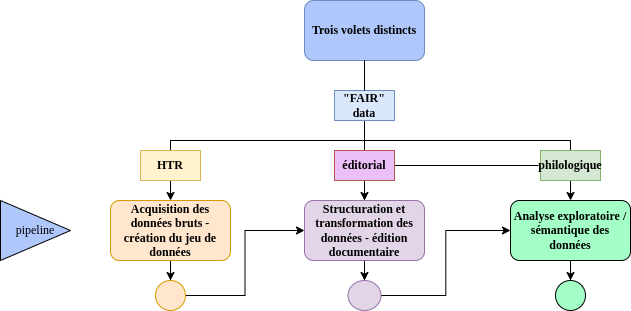
\includegraphics[width=13cm, height=6cm]{pipeline/volets_projet.png}
    \caption{Aperçu logique du pipeline suivi. Trois niveaux de traitement successifs, de la transcription à la structuration et la visualisation des données.}
\end{figure}

Par conséquent, la méthodologie adoptée consiste à développer un pipeline qui couvre toutes les étapes de la méthodologie scientifique, de l'acquisition des données initiales brutes à la génération des résultats finaux ayant comme point de départ la réalité matérielle des différents témoins manuscrits. Les tâches automatisées sont interconnectées pour former un flux cohérent, tout en conservant leur autonomie pour tirer parti des résultats de chaque étape de manière indépendante. Le pipeline fait usage d'outils existants, testés et validés par la communauté scientifique, afin de favoriser l'interopérabilité tout en prenant en compte les spécificités et les besoins propres à notre projet.\\

Les avantages de cette approche sont doubles : elle offre à la communauté des paléographes des outils pour traiter de manière plus efficace et rapide la nature complexe de leur sujet d'étude, et fournit aux chercheurs en sciences humaines et computationnelles des jeux de données (\textit{Ground Truth\footnote{La verité de terrain consiste en\og{}des ensembles de données annotées et corrigées de manière à fournir au modèle des paires composées d'une part d'une image ou d'une portion d'image (entrée) et d'autre part de l’annotation attendue (sortie), qui peut être des coordonnées dans le cas de la segmentation ou un ensemble de caractères pour la transcription. Les performances des modèles dépendent certes de l'architecture neuronale mise en place, mais aussi de la qualité et de la quantité de vérité de terrain fournies lors de l'apprentissage.\fg{} Définition tirée de \cite{chague2021htr}}}) pour l'entraînement de modèles d'apprentissage machine et tester leur limites, notamment quand il s'agit des données complexes.\\

Sur le plan éditorial, cette approche privilégie un format numérique, déjà adopté par la communauté scientifique, qui facilite le stockage et la gestion de données complexes, à savoir multifacettes et hiérarchiques. Ce modèle favorise l'accessibilité et l'interopérabilité des données, ce qui permet une meilleure utilisation et mise en valeur des informations. De plus, d'un point de vue philologique, cette approche apporte une contribution significative en rendant l'étude des gloses plus objective et quantifiable car ,en utilisant des méthodes numériques, il devient possible d'analyser les gloses de manière systématique et d'obtenir des résultats mesurables et vérifiables. \\

L'objectif ultime de cette approche est de démontrer comment l'utilisation de la lecture distante, peut compléter de manière efficace et enrichir la lecture proche. Plutôt que de se concentrer exclusivement sur une analyse détaillée d'un texte spécifique, la lecture à distance permet une exploration plus large et une analyse statistique et comparative des données textuelles, offrant ainsi une perspective complémentaire et nuancée des textes étudiés, en tirant parti des avantages respectifs de chaque approche\footnote{Sur les avantages d'une paléographie statistique voir \cite{stutzmann2011paleographie}}. Cela ouvre de nouvelles possibilités et perspectives dans le domaine des manuscrits glosés et permet une meilleure compréhension de leur tradition manuscrite dans leur ensemble.

\chapter{État de l'art}

Notre choix d'étudier la tradition manuscrite du \textit{de uerbo} d'Eutychès est motivé par plusieurs raisons:  \\
\begin{itemize}
    \item Premièrement, le matériel étudié est largement inédit, offrant ainsi une opportunité de contribuer à la recherche en apportant de nouvelles réflexions sur cette œuvre;
    \item Deuxièmement, la tradition manuscrite du \textit{de uerbo} d'Eutychès n'est pas vaste en termes de taille, ni illimitée en termes de frontières géographiques et temporelles. Cette particularité la rend plus accessible à l'analyse, facilitant ainsi une approche plus ciblée et une meilleure appréhension des des témoins disponibles;
    \item Troisièmement, grâce au travail des chercheurs dans le domaine des grammairiens latins et leur tradition manuscrite, il existe une littérature riche qui va nous servir de guide pour nos analyses. Cette richesse de références et d'analyses préexistantes constitue une base solide pour notre étude, vis à vis de laquelle nous pouvons tester notre méthode et résultats;
    \item Enfin, notre choix est motivé par notre familiarité avec le contenu grammatical des traités grammaticaux dits \textit{regulae} de l'Antiquité tardive, ayant déjà étudié la grammaire de \textit{Charisius} dans le cadre de notre M2 en Latin à la Sorbonne.
\end{itemize}

\section{Eutychès  et son \textit{De uerbo}}

On place le grammairien Eutychès (\textit{alias} Eutex, Eutychius) à Constantinople au milieu du \textsc{vi}\ieme{} siècle\footnote{ Ce sous-chapitre constitue une compilation des informations dans \cite{lomanto1985Eutiche}, \cite{conduche2019miseenpage} et \cite{zetzel2018critics}p.298}. Disciple de Priscien de Césarée (qu'Eutychès défint en tant que \textit{meus preceptor}\footnote{\cite{keil1857grammatici}, vol5, p.456}), sur le plan de la doctrine grammaticale,  l'oeuvre d'Eutychès constitue le premier témoin de sa postérité. Auteur de deux traités grammaticaux, le premier, le \textit{De aspiratione}, traite le \textit{h} graphique (aspiration) en la langue latine et nous est transmis seulement via la tradition indirecte, à savoir grâce au chapitre  \textsc{ix} \textit{De aspiratione},du \textit{De orthographia} de Cassiodore. C'est seulement le deuxième traité, à savoir le \textit{De uerbo} qui nous est parvenu et jouit d'une tradition directe bien documentée, et qui constitue le sujet de notre recherche.\\

Dans cet essai grammatical articulé en deux livres \footnote{annoncé par l'auteur lui même dans : \textit{GL},vol.5,p.447, 12-14 \textit{ad discernendas pertinens coniugationes, duobus libellis inclusi. Quorum prior obseruationibus instruitur generalibus, alter inditio finalitatis, spetiales exequitur regulas.}}, Eutychès répond à la requête de son disciple, \textit{Craterus}, qui s'interroge sur la méthode permettant d'attribuer correctement les verbes latins à leur modèle de conjugaison respectif à partir de leur forme de base, à savoir la première personne du singulier du présent de l'indicatif (à l'époque considérée). L'auteur s'engage dans ce traité à définir les critères formels permettant de déterminer l'appartenance des verbes latins à une conjugaison spécifique. Après avoir exposé quelques principes généraux, tels que l'appartenance des verbes inchoatifs à la troisième conjugaison, Eutychès examine une liste finie de suffixes de dérivation verbale et nominale. Il distingue ainsi les verbes dérivés, dont l'appartenance à un modèle de conjugaison dépend de leur suffixe, des formes primaires, où l'indice réside dans leur famille lexicale. L'auteur procède ensuite à une analyse minutieuse des \textit{finalitates verborum}, c'est-à-dire des sons ou groupes de sons précédant la désinence -o/-or, en indiquant le type de flexion auquel chaque \textit{finalitas} est caractéristique. Cette analyse, parfois réduite à des schématismes, se distingue par son style simple et aride, abondamment illustré par des listes d'exemples, qui se répètent afin de faciliter la compréhension. Il convient de noter que dans cette analyse, de nombreux passages tirés d'auteurs classiques sont illustratifs. En effet, Eutychès ne soulève pas de doutes ni ne discute de cas controversés, mais décrit avec soin les phénomènes propres à la langue latine, sans faire de distinctions entre l'usage courant et l'usage littéraire.\\

Sa méthode a été critiquée par certains philologues qui n'y reconnaissait pas une valeur intrinsèque, un apport grammatical doctrinal conséquent. Cette approche reflète la tendance générale des chercheurs dans le domaine des GL jusqu'au milieu du \textsc{xx}\ieme{} siècle où, l'intérêt croissant pour la linguistique et l'histoire des la pensée linguistique, a entraîné un renouveau dans l'étude des grammairiens latins dans un cadre plus scientifique\footnote{Viven Law, Louis Holtz, Mario DeNonno et Paolo de Paolis ne sont que quelques-uns des noms qui ont mené des recherches pionnières dans ce domaine.}. \\

En ce qui concerne la littérature sur les manuscrits d'Eutychès, ce n'est qu'en 1974 que Jeudy Colette a entrepris un recensement exhaustif de la tradition directe du \textit{De uerbo}\footnote{\cite{jeudy1974manuscrits}. \href{http://www.mmdc.nl/static/site/index.html}{Le site MMDC} mentionne sur le codex composite Leiden, UB : ms. BPL 154 : 1, ff. 001-037 \og{} This text is a compilation of excerpts from Priscian's Institutiones grammaticae and from Eutychès' Ars de verbo \fg{}, information d'ailleurs nulle part mentionnée dans la littérature. Le ms. en question n'étant pas numerisé, cette information reste à vérifier.}. Son étude a permis d'identifier vingt-neuf témoins manuscrits du \textit{De uerbo}, qu'ils soient complets ou fragmentaires, glosés ou non. Ces témoins couvrent une période allant du \textsc{viii}\ieme{} au \textsc{xi}\ieme{} siècle.\\

En ce qui concerne la postérité de l'œuvre d'Eutychès, qui témoigne de son succès au Haut Moyen Âge, sa diffusion en Occident a commencé assez rapidement, peut-être même de son vivant, mais certainement avant la fin du \textsc{vi}\ieme{} siècle, date à laquelle est située l'œuvre de Cassiodore. Son traité a été lu et utilisé jusqu'au \textsc{xi}\ieme{} siècle,  comme en témoignent à la fois la tradition directe et indirecte qui entoure le traité, ainsi que les commentaires qui lui ont été consacrés. En ce qui concerne l'étendue géographique de son influence, le \textit{De uerbo} doit indubitablement sa renommée aux Irlandais, car les deux témoins les plus anciens\footnote{le  premier  copié  au \textsc{viii}\ieme{} à  Bobbio  Naples,lib naz. Lat.2 (malheureusement passé au réactif),  le  deuxième  en  Irlande même,  avec  des gloses  irlandaises : Il s'agit des deux fragments BnF. Lat 10400  et 11411.} sont rédigés en minuscule irlandaise. À partir du début du \textsc{ix}\ieme{} siècle, on constate la présence de ce manuel également en Angleterre et sur le continent, dans l'ensemble de l'empire carolingien, avec une concentration particulière dans trois régions : la France (surtout dans le Nord et l'Est), la Bavière et la région du lac de Constance. Ces manuscrits se retrouvent principalement dans des milieux monastiques tels que Luxeuil, Corbie, Saint-Gall et Fleury, entre autres.\\


Outre sa diffusion sous forme manuscrite, la renommée du \textit{De uerbo} est également attestée par son utilisation indirecte dans les grammaires du Haut Moyen Âge. C'est Bengt Löfstedt, éditeur de plusieurs de ces grammaires,  \footnote{\cite{lofstedt1965der} puis \cite{lofstedt1972zu}p. 47-65.}, qui a attiré l'attention sur la présence d'Eutychès parmi leurs sources. Cette tradition indirecte remonte d'au moins un siècle avant les plus anciens manuscrits conservés, à la seconde moitié du \textsc{vii}\ieme{} siècle, avec le traité anonyme intitulé \textit{Ad Cuimnanum}, du nom de son dédicataire. Par la suite, tout au long de la période carolingienne, les grammairiens ont continué à exploiter le \textit{De verbo} dans la rédaction de leurs propres traités, notamment Sedulius Scottus et Rémi d'Auxerre, dont nous parlerons ultérieurement en ce qui concerne leur format. Il est également important de noter, que la dernière édition critique de l'oeuvre principale date du \textsc{xix}\ieme{} siècle et est en grande partie obsolète, que l'ensemble des gloses et le commentaire de Rémi restent largément inédits, et seul le commentaire de Sedulius, qui fait partie de la tradition indirecte, jouit d'une édition scientifique récente\cite{scottus1980donati}.\\

\section{La typologie des manuscrits grammaticaux latins}

\begin{flushright}\textit{ « Literary theory throughout the medieval period presupposes the manuscript form of the text, a form with its own distinctive features such as textual variation from copy to copy and the encoding of script and page layout within a total system of verbal and visual meanings »}\end{flushright}

\begin{flushright}Martin Irvine, \textit{The Making of Textual Culture}, p.17 \end{flushright}


La tradition manuscrite des textes grammaticaux se distingue par deux caractéristiques intrinsèques universellement présentes : une mise en page complexe et la présence de gloses. Louis Holtz, érudit et théoricien majeur dans le domaine des manuscrits grammaticaux, résume ces caractéristiques codicologiques globales qui constituent le noyau du système, dans son article intitulé \fg{} \footnote{\cite{holtz1978typologie}, p.247} :

\blockquote{[...]type d'écriture, mise en page, recours aux abréviations, décoration. Tous ces éléments, dans la mesure où ils participent d'un système donné, ont leur importance pour rendre compte aussi bien de la survie des textes transmis que pour expliquer la forme particulière dans laquelle il nous sont parvenus. [...] ces éléments proprement codicologiques, qu'un chercheur, dès lors qu'il a recours à ce document qu'est le manuscrit, ne peut éluder, même s'il n'a en vue qu'une édition critique, car ils sont susceptibles d'éclairer ou d'amplifier les données auxquelles lui donne accès le collationnement du texte lui-même.} 

\subsection{Les tableaux d'exemples}

Plusieurs témoins présentent des exemples de conjugaisons verbales disposées en colonnes, qu'elles soient ordonnées ou non. Outre leur utilité pour faciliter la lecture et la mémorisation des exemples, ces colonnes pourraient également refléter l'usage concret du document copié, tout en donnant un aperçu des témoins disponibles aux copistes et des œuvres grammaticales en circulation pendant le Moyen Âge. Vivien Law dans son article « From aural to visual » \footnote{\cite{law1997aural}}, considère que la présentation tabulaire est un indice du caractère principalement oral de la grammaire. Elle établit un lien entre la représentation visuelle, l'utilisation de diagrammes dans la grammaire et les progrès de l'analyse morphologique\footnote{cf. également le chapitre \og{}Memory and Structure of Grammars\fg{} de Vivien Law dans le premier volume de \cite{denonnomanuscripts} pour une analyse plus détaillée.}.\\

Et si Remigio Sabbadini, responsable d'une collation partielle du codex glosé Milan, Ambr. B71sup.\footnote{\cite{sabbadini1995opere},p.76-83}, avait raison de déplorer l'impossibilité de restaurer le texte d'Eutychès dans sa forme originale et la futilité d'amasser des collations, du fait que chaque copiste modifiait ou changeait cette liste à sa guise en transcrivant horizontalement les colonnes verticales et vice versa, cette observation n'est pas en vain pour la fortune du texte tout court. Pour le cas d'Eutyche, un examen approfondi\footnote{L'étude unique qui porte sur cette question est la suivante, dotée d'un tableau comparatif des occurrences des listes ordonnées dans la tradition manuscrite : \cite{conduche2019miseenpage}.} des tableaux ordonnés des exemples dans la tradition manuscrite, comparés aux \textit{artes} influencées par\textit{ De uerbo}, démontre l'importance d'une telle analyse.


\subsection{Le couple indissociable lemma-glose}

Vu le nombre important de témoins glosés présents dans la tradition manuscrite du \textit{De uerbo}, il est crucial de les définir brièvement et d'explorer la nature et la fonction des gloses en tant qu'instrument textuel pour la transmission des savoirs. Comme c'est le cas pour de nombreuses œuvres classiques influentes, ainsi que des œuvres bibliques et des manuels pratiques tels que les ouvrages juridiques, les espaces interlinéaires et marginaux d'un manuscrit des \textit{artes} sont généralement remplis de gloses.
La clarté et la résolution des incertitudes sont des préoccupations fondamentales pour le glossateur en principe. Malgré les difficultés ponctuelles, les gloses interlinéaires sont généralement concises, limpides et exemptes d'ambiguïté et ainsi leur capacité à guider le lecteur et leur valeur pédagogique sont indéniables. Louis Holtz\footnote{\cite{holtz1984gloses}, p. 142} propose une définition des éléments textuels secondaires en tant que : \og{}tout ce qui vient s'ajouter au texte d'un auteur après coup [...] qui n'a d'autre raison d'être que de faciliter, de guider, d'orienter la lecture [...] en somme, tout ce qui, dans nos manuscrits, n'émane pas directement de l'auteur lui-même...\fg{}. Franck Cinato explore le concept et le statut des gloses dans le contexte grammatical\footnote{\cite{cinato2015priscien}, p. 187-198} et propose sa propre définition \textit{ontologique} : \blockquote{toute augmentation péritextuelle qui précise ou diversifie l'information contenue dans un texte principal.} Cela permet, à une échelle codicologique, de \og{}documenter la postérité intellectuelle des idées\footnote{\cite{dinkova2020text}, p. 924}\fg{}.\\

Effectivement, l'étude de ce paratexte riche et complexe permet d'éclairer la réception des \textit{artes} et la tradition des études grammaticales tant dans l'Antiquité tardive que durant le Moyen Âge. Ces gloses ont récemment suscité un intérêt croissant dans la recherche \footnote{\cite{monella2019digital}}. Étant donnée la variété des gloses apposées sur le texte grammatical (simple synonymes, notes qui élucident le texte, observations grammaticales etc.) celui-ci offre un exemple manifeste de la relation dynamique entre le texte et le paratexte et notamment entre le mot ou groupe de mots nécessitant élucidation, le \textit{lemme}.\\

Ayant abordé ces deux termes, il est nécessaire d'établir une distinction sémantique et fonctionnelle entre le texte et le paratexte auquel les gloses appartiennent. En général, la glose vise à clarifier le sens de certaines phrases et même de certains mots (\textit{non solum sententiam sed etiam verba attendit}\footnote{Pour l'évolution sémantique du terme de l'Antiquité au Moyen Âge, voir \cite{holtz1996glossaires}}). Le texte, quant à lui, correspond au livre de l'auteur glosé et ne comporte pas d'autres remarques explicatives (\textit{textus est liber sine littere vel sententie ex positione})\footnote{\cite{dinkova2020text}, p.925}, où les mots deviennent autant de lemmes potentiels. Cependant, la frontière entre le texte et le paratexte peut parfois être poreuse, notamment lorsque les lemmes sont remplacés par des gloses, un phénomène certainement pas rare. Cette confusion a suscité de nombreux débats et entraîné de multiples définitions concernant le sens des \textit{marginalia}, des notes, des commentaires et des gloses\footnote{Pour une vue d'ensemble de l'espace paratextuel des manuscrits, voir notamment le chapitre d'Adolfo Tura intitulé \og{}Essai sur les \textit{marginalia} en tant que pratique et documents\fg{} dans \cite{jacquart2005scientia}}. En réalité, il existe d'innombrables \og{}niveaux de paratextualité\fg{} en fonction de la localisation et de la fonction d'une glose. On trouve également un troisième niveau de paratexte, étroitement lié aux gloses et aux marginalia, à savoir les glossaires à part entière. Ces glossaires avaient pour rôle de fournir une aide à la compréhension de base de la construction du texte.\\

Cinato (2015) a élaboré un tableau explicatif des relations entre les différents niveaux de paratextualité dans le cas des témoins glosés de Priscien, et illustre la diversité et l'interconnexion des différents niveaux de paratextualité qui créent un réseau de connaissances, dont le point de référence est le texte-lemme mais qui s'étend bien au-délà.

\begin{figure}[ht]
  \centering
  \includegraphics[height=9cm, width=9cm]{modelisation_graphs/Cinato-page-horspage.png}
  \caption{Niveau de paratexte selon la proximité au lemme.}
  \label{fig:exemple}
\end{figure}

Récapitulatif: Comment désigner alors les ajouts de dimensions variables qui se donnent rendez-vous dans les marges des manuscrits : gloses, scolies, commentaires marginaux? Il existe de états matériels distincts de gloses qui servent des objectifs spécifiques \footnote{\cite{holtz1995glosse}, p.65-75} :

\begin{enumerate}
  \item Glose interlinéaire : se trouve \textit{in situ} et analyse \textit{ad litteram} - au mot à mot - le texte, en étroite dépendance du lemme nécessitant explications;
 \item Glose marginale : constitue l'extension immédiate de la glose interlinéaire, elle plus longue et situé en marge, bien que de façon pas systématique;
 \item Commentaire marginal \textit{in catena} : constitue une forme hybride d'annotation, entre glose marginale et \textit{scholie} autonome. Tous les éléments gardent leur apparente autonomie (cf. fig 2.1). L'œil fixe tantôt le corps du texte, tantôt les marges; La différence entre glose marginale simple et commentaire courant, et que  les commentaires sont compilés à partir de multiples ensembles de gloses marginales ; ils sont codifiés et organisés ;\footnote{Pour les deux traditions, voir \cite{teeuwen2015carolingian} et l'excellente Introduction de Christina Stuttleworth Kraus: \cite{kraus2002introduction}. Dans le projet \og{}Marginal Scholarship\fg{}, le terme \textit{commentary} est défini ainsi: Commentary, in our terminology, is a ‘set’ body of annotations copied into a manuscript in the margin and/or interlinear space. It contrasts with ‘ad-hoc’ annotations or spontaneous annotations, which can be expected to be individual notes made by students or readers on the spot[...]The difference between a commentary and annotations is not necessary strict and depends on whether the annotations display a certain design or unity (e.g. because they were all entered by the same hand, because they can be shown to reflect a single purpose or theme, or because the manuscript was from the outset intended for the insertion of marginal text).}
 \item Commentaire continu : il s'agit d'un genre bien délimité, il est soumis à une tradition manuscrite propre et reçoit les mêmes attentions que n’importe quelle œuvre littéraire, dans la mesure où il n’est pas transmis anonymement.
\end{enumerate}

\section{De la Glose au Commentaire - Considérations théoriques}

Des niveaux variés de sophistication de la glose sont souvent mis en jeu simultanément, reflétant les besoins intellectuels d'un lectorat spécifique. Notamment dans le cadre de l'enseignement, la complexité des annotations témoigne du niveau d'éducation auquel les textes étaient intégrés dans le programme. Certains manuels médiévaux comportent même plusieurs couches de gloses, introduites indépendamment par différents utilisateurs au fil du temps. Dans de tels cas, les gloses entrent en dialogue non seulement avec le texte lui-même, mais aussi avec les autres annotations présentes. Même lorsqu'elles résultent d'une lecture et d'une étude privées, les gloses individuelles varient en termes de difficulté et d'objectif, reflétant les intérêts savants de leur auteur. Par conséquent, la composition principale et les commentaires secondaires exercent l'un sur l'autre une influence réciproque, donnant naissance à une nouvelle réalité textuelle à la fois plus riche en sens et plus complexe dans sa forme. Il ne suffit pas de considérer les gloses et les commentaires comme de simples élucidations de textes obscurs et difficiles. La pratique de la glossologie médiévale dépasse largement cette fonction. Elle représente un mode de pensée, une forme d'expression et une méthode complexe d'engagement intellectuel avec la tradition littéraire et érudite transmise\footnote{\cite{dinkova2020text}, p.938}. Suivre un tel processus est crucial pour l'histoire des idées, la transmission et la postérité des textes, ainsi que pour l'enseignement de la grammaire. Cela revêt une importance particulière dans le cas d'une œuvre aux dimensions multidimensionnelles, allant du texte principal et de ses gloses aux commentaires externes et aux glossaires.\\


Pour examiner de plus près le contexte historico-culturel, à la fin de l'Antiquité tardive et au tournant de l'époque carolingienne, les manuels de grammaire latine ont connu un renouveau grâce à leur contenu éducatif riche, adapté aux besoins d'un nouveau public. Une différence fondamentale entre la grammaire antique et celle que nous trouvons dans les manuscrits médiévaux réside dans le fait que cette théorie linguistique ne s'adresse plus au même auditoire. En effet, l'enseignement du latin à un public hellénophone au \textsc{vi}\ieme{} de son enseignement aux peuples germaniques, aux Irlandais et aux Anglo-Saxons aux\textsc{viii}\ieme{} et \textsc{ix}\ieme{} siècles. Pour citer James E.G. Zetzel : \blockquote{The orthographic reforms of Alcuin were only one part of a large change visible in scholarly writings. In grammars, where the evidence is clearest, by the late eighth century there begins to be a distinction between the late antique grammatical texts as independent and coherent works on the one hand, and whatever newer scholars choose to write about them, or about their subjects. The boundary between text and commentary, between past and present, was restored  \\ \footnote{\cite{zetzel2018critics} p. 227}.}

Ainsi les traités grammaticaux manifestent une remarquable faculté d'adaptation, et ceci se matérialise dans nos recueils du haut Moyen Âge par un fait massif, dont il doit être tenu le plus grand compte : il est rare que les textes grammaticaux antiques nous parviennent nus, coupés des commentaires qui constituent leur mise à jour médiévale. Il est même improbable que les oeuvres grammaticales aient été transmises sans modifications au texte principal, contrairement aux oeuvres poétiques ou autoritaires. Le livre de grammaire est un manuel utilisé et son contenu est adapté en fonction des besoins de l'époque. À cause des conditions de la transmission manuscrite, lorsque nous croyons comprendre une typologie figée des manuscrits de grammaire, nous sommes déjà au Haut Moyen Âge, que ce soit dans la zone insulaire ou sur le continent, sous l'influence de la Renaissance carolingienne\footnote{ \cite{holtz1995glosse}.}. Aujourd'hui encore, nous devons la survie des grammaires de l'Antiquité tardive aux techniques de remaniement et d'adaptation des maîtres irlandais et carolingiens.\\

La tradition manuscrite du \textit{De verbo} d'Eutychès, bien qu'elle ne diffère pas fondamentalement des autres ouvrages grammaticaux de l'Antiquité tardive, présente certaines particularités qui en font un cas d'étude intéressant pour l'élaboration et l'analyse de sa réception à l'époque carolingienne. Parmi la trentaine de témoins de la tradition directe recensés par Colette Jeudy\footnote{\cite{jeudy1974manuscrits}}, une grande partie des manuscrits qui nous sont parvenus sont annotés à différents degrés, certains portant des notes tironiennes ou des notes en cryptographie, annotés en latin ou en langue vulgaire : irlandaise, bretonne, allemande ou française. Ce qui est de plus, deux commentaires de nature différente ont survécu et nous sont parvenus jusqu'à aujourd'hui ; le premier est le commentaire continu de Sedulius Scottus, savant irlandais, qui a rédige au milieu du \textsc{ix}\ieme{} siècle (en plus de la théologie et de la poésie) un certain nombre de commentaires grammaticaux. Néanmoins, ce type de commentaire continu rentre plutôt dans le domaine de la tradition indirecte et constitue un texte à part entière. Dans un tout autre style que Sedulius, Rémi d’Auxerre (v. 841-908) en fit aussi un commentaire, conservé sous la forme des gloses marginales anonymes, aux fol. 81-97 du ms. 1470 de la Bibliothèque municipale de Rouen, reproduites aussi dans le codex  BnF, lat. 7499 \footnote{\cite{jeudy1974manuscrits},p. 434-436. On précise que le commentaire de Rémi d'Auxerre reste largement inédit \cite{zetzel2018critics},p. 352. La seule édition à ce jour est partielle : \footnote{\cite{manitiusremigiusscholien}}}. En bon philologue, il s'intéresse aux diverses leçons  des  manuscrits qu'il a sous les yeux et aux divergences d'interprétation : \textit{Caluesco }(448, 28) : \og{} Alii codices habent caluisco id est caluere incipio, id est decipere, et alii caluesco, id  est caluus fieri incipio \fg{} (Paris 7499, fol. 73 v)., ce codex hybride comporte le texte, les gloses et le commentaire de Rémi en marge, fait partie intégrale de la tradition à la fois du texte principal et des gloses y associées, étant donnée qu'il avait accès aux matériels aujourd'hui perdus, qui complimentent la tradition manuscrite de l'oeuvre \footnote{\cite{holtz1978typologie},p.258 section \og{} De la glose anarchique au commentaire organique\fg{} et p.260 \og{} Fluidité des systèmes\fg{}.}. Dans ces conditions, il serait imprudent de séparer en deux lots les opuscules d'un manuscrit grammatical et de n'accorder qu'une attention faible aux commentaires médiévaux et au lien étroit qu'ils entretiennent avec l'oeuvre originale. Ce serait se priver de nombreuses sources d'information sur le texte antique lui-même, sa transmission, la qualité de sa recension, le lieu où il a été copié, informations qui font souvent défaut pour d'autres types de textes. La manière dont les lecteurs contemporains et tardifs de ces textes ont réellement donné un sens à leur doctrine et l'ont appliquée en dehors du domaine immédiat de la grammaire sont des domaines d'étude qui commencent tout juste à attirer l'attention. Comment les grammairiens du \textsc{v}\ieme{} et \textsc{vi}\ieme{} siècles étaient lus par les grammairiens des \textsc{x}\ieme{} et \textsc{xi}\ieme{} - ce que les historiens de la linguistique aimeraient savoir.\\

Pour conclure cette partie théorique et pour en résumer les points centraux, à l'inverse des œuvres littéraires, les grammaires latines ont été copiées au cours des siècles non pour leur \og{}valeur intrinsèque \fg{} mais en tant que manuels scolaires, selon l’utilité concrète et l’intérêt qu’elles présentaient en termes d’apprentissage du latin. Pour cette raison, selon le niveau d’érudition et les besoins pratiques, les copistes/compilateurs, eux-mêmes souvent érudits, proposent des synonymes, des gloses, des corrections et des commentaires en marge et souvent reproduisent des tableaux d'exemples et d'exceptions. Ceci rend la typologie des manuscrits grammaticaux multidimensionnelle, étayée et en quelque sorte personnalisée dans chaque témoin, tout en gardant un rapport d'interdépendance entre eux. Nous avons dit des manuscrits grammaticaux que ce sont des instruments de travail et leur mise en page incarne leur rôle pédagogique. En même temps, en tant que \textit{custodes Latinitatis}, les traités des grammairiens, sont très précieux dans l’aperçu de l’enseignement de la grammaire, la littérarité et l’évolution linguistique pendant l’Antiquité tardive. Soit via la doctrine linguistique qu’ils présentent, soit via le renvoi – par le biais de citations – aux œuvres littéraires et grammaticales perdues, ils contribuent au \textit{continuum} intellectuel. Leur popularité pendant le Moyen Âge, qui se traduit en de nombreuses copies de leurs œuvres, témoigne de l’état de l’apprentissage du latin sur le continent européen à cette période là.\\


Au début de notre recherche de Master en Humanités Numériques, l'objectif était plutôt d'examiner seule la transmission des gloses, leur typologie et leur forme, à l'instar du travail de Cinato sur Priscien\footnote{\cite{cinato2015priscien}}, qui était parmi des premiers chercheurs à les possibilités d'un corpus électronique pour une analyse croisée à large échelle des gloses attribuées aux oeuvres grammaticales. Pourtant, la spécificité matérielle et structurelle du commentaire de Rémi d'Auxerre, cet heureux accident de la tradition manuscrite, nous a inspiré de modéliser et de trouver une façon de \textit{mesurer} l'impact de la tradition antérieure des gloses (old, anonymous gloss tradition) à la confection de son commentaire courant.\\


\section{Description du corpus - MsDesc}

Pour mener à bien une étude si délicate, à savoir modéliser le processus de passage entre l'ancien matériel de gloses et le commentaire structuré, il est nécessaire de sélectionner des témoins qui correspondent aux critères formelles, chronologiques, et de provenance spécifiques, afin de créer un corpus cohérent.\\

Selon la littérature \footnote{\cite{oSullivanglossae}, Introduction p.XX}, les centres intellectuels les plus prometteurs pour ce domaine de recherche sont Corbie, Laon et Auxerre-Fleury. Ces centres refont surface lorsque l'on étudie la transmission des textes classiques et grammaticaux au début du Moyen Âge et l'érudition qui les entoure \footnote{voir. aussi \cite{oSullivan2017lemma}, p. 376. \cite{irvine1994making}, p. 392 \og{}This format [sc. text, gloss and commentary] was instituted and perpetuated in centers of institutional powers - Tours, Corbie, Fleury, Reims, Auxerre, St. Gall, Canterbury, Abingdon, Worcester, Durham - and served the needs of the schools and libraries in these centers learning and authority.\fg{}}. Suivant le contexte historique, c’est vers la fin du \textsc{ix}\ieme{} siècle que Rémi d'Auxerre, entre autres, a été appelé à Reims par l'archevêque Foulques (882-900), pour rénover les écoles \footnote{\cite{jeudy1974manuscrits}}.\\

Alors, quels témoins choisir? La tradition manuscrite d'Eutychès étant assez limitée, il y a peu de manuscrits qui répondent à tous les critères et qui sont disponibles. Parmi ceux-ci, nous avons identifié trois manuscrits fortement glosés, un manuscrit contenant le commentaire marginale de Rémi d'Auxerre, ainsi qu'un glossaire. Tous ces manuscrits ont été copiés dans les\textit{ scriptoria} du Nord et du Nord-Est de la France, notamment à Reims, Auxerre, Fleury et Corbie et ils datent tous du début du \textsc{ix}\ieme{} et le \textsc{xi}\ieme{} siècles.\\

Parmi la liste des manuscrits recensés en 1974 par Jeudy Colette, nous avons choisi en tant que jeu de données, après discussion d'abord avec Mme Conduché et ensuite avec M Franck Cinato, les suivants, dont nous donnerons une brève description :\\


\textsc{le BnF Latin 14087} \\


Le manuscrit en question, datant du début du \textsc{ix}\ieme{} siècle, a été copié dans l'abbaye Saint-Pierre de Corbie \footnote{Notice en ligne : \url{https://archivesetmanuscrits.bnf.fr/ark:/12148/cc87895}}. Les folios 97 et 98 du manuscrit contiennent des \textit{Glossae super Eutychen}.\\

\textsc{le Staatsbibliotek, Bamberg Msc. Class 30}\\

Ce \textit{codex}, datant du 3e quart du \textsc{ix}\ieme{} siècle et provenant de Reims, comprend un contenu grammatical varié. Il contient tout d'abord l'\textit{Ars grammatica} de Clemens Scotus, suivi de l'\textit{Ars de uerbo} d'Eutyches (ff.71-85), ainsi que le \textit{Compendiosa doctrina} de Nonius Marcellus. Les gloses interlinéaires présentes dans le manuscrit sont toutes de la même main\footnote{Selon la notice du manuscrit : \cite{leitschuh1966katalog}, p.1063 (chapitre F.Classikerhandschriften p.31) disponible en ligne : \url{http://bilder.manuscripta-mediaevalia.de/hs/katalogseiten/HSK0600_1063_jpg.htm}}.\\

\textsc{le BnF Latin 7499}\\

Selon la notice de la BnF \footnote{Rédigée par Clémence Pelletier en 2021 : \url{https://archivesetmanuscrits.bnf.fr/ark:/12148/cc1253930}} ce \textit{codex} est composé de trois unités, dont les deux premières (ff. 1r-62v et 63r-71v) contiennent les livres XVII-XVIII des \textit{Institutiones grammaticae} de Priscien ; les \textit{Carmina} d'Engelmodus Suessionensis ; la \textit{Periegesis} de \textit{Dionysius Periegeta} traduit par Priscien, et finalement des anonymes Notes sur Priscien, auxquelles une troisième a été annexée. \\

La troisième unité, qui contient le \textit{de uerbo} d'Eutychès est un peu plus tardive, de la première moitié du \textsc{x}\ieme{} siècle, datée par C. Jeudy \footnote{ \cite{jeudy1974manuscrits} p. 431}  et contrairement aux deux précédentes, elle n’aurait pas été copiée à Corbie, mais, toujours d’après C. Jeudy, elle viendrait d’un \textit{scriptorium} proche de Corbie et sous influence irlandaise. Elle a toutefois sans doute appartenu elle aussi à Corbie durant le bas Moyen-Âge. Cette unité est identifiée par C Jeudy \footnote{\cite{jeudymanuscritMilan}} et Manitius \footnote{\cite{manitius1911karolongischen}} avec le commentaire de Rémi d'Auxerre.\\

Quant à sa composition codicologique: 11 cahiers, pour la plupart des quaternions (f. 1-8, 9-16, 17-24, 25-32, 33-40, 41-48, 49-56) ainsi qu’un ternion (f. 57-62) et un quinion (f. 72-81). Deux quaternions ont reçu des feuillets additionnels (f. 63-70, auquel a été rattaché le f. 71 ; et f. 82-89, auquel ont été rattachés les f. 90-91).\\
 

\textsc{le VLO41}\\

Nous allons nous tarder un peu plus sur ce manuscrit, qui présente des spécificités paléographiques qui sont très intéressantes à l'analyse. Le manuscrit inédit  Leiden, Vossianus Latinus \textit{in octauo} 41\footnote{Dorénavant VLO41.}, que Keil a écarté en tant que \textit{codex descriptiuus} lors de son édition. Il s'agit d'un \textit{codex} composite, qui accueille presque exclusivement des ouvrages grammaticaux, le  \textit{De uerbo} d'Eutychès et les \textit{Etymologiae} d'Isidore de Séville. D'abord une brève description : VLO41 est un manuscrit en parchemin du dernier quart du \textsc{ix}\ieme{} siècle qui compte  65 folios paginés en haut à droite. La feuille de garde (1r) consiste en une liste de la correspondance de Grégoire le Grand.\\

Quant à sa composition codicologique,  les folios sont disposés en 8 cahiers de taille non homogène, à savoir : IV (2-9) + V (10-19)+ IV (20-27) + III (28-33) (fin de l'oeuvre d'Eutychès) + 4 IV (34-65). Le codex manque un feuillet dechiré entre les folios 9v et 10r ce qui coincide au passage du quaternion(à l'origine un quinion) au deuxième quinion. Par contre le sens de lecture n'est pas perturbée et la main reste la même jusqu'au folio 22r. On note ici que les 33 premiers folios du manuscrit qui comportent l'oeuvre d'Eutychès correspondent à la deuxième unité codicologique \footnote{\cite{de1973codices},p.80}.Le manuscrit, d'après une comparaison avec le codex \textit{VLO}37, doit avoir appartenu au \textsc{xii}\ieme{} siècle à l'abbaye de Fleury (DeMeyier\footnote{\cite{de1973codices},p.81.} : \textit{33v scriptura evanuit ; insuper custos quidam bibliothecae Floriacensis (?) xii litteris maioribus ab imo ad summum codicis indicem scripsit : Liber Ysidori iunioris cu(m) euticio grammatico ; cf. ad cod. O.37}).\\

Un total de quatre mains principales et huit mains de glosateurs participent à la confection du manuscrit, qui s'étendent sur plus d'un siècle (DeMeyier considère, d'après l'écriture, que les mains de gloseurs appartiennent entièrement au \textsc{x}\ieme{} siècle). Le manuscrit comporte plusieurs essais de plume, dont une série de neumes de la séquence \textit{Virgo inuiolata}, le mot in-uiolata figurant en-dessous des neumes. Une souscription d'un certain copiste Concardus au folio 25r et une incertaine ou effacée (\textit{mihi nom̃ ++ inđ erit/ uer?u}m) dans la marge du folio 9v sont également présentes. \\
Selon sa typologie, VLO41 constitue un cas particulièrement intéressant qui correspond au type $\Gamma$. Plus particulièrement il est question d'une grammaire glosée, d'une collection propre à un témoin manuscrit unique où les gloses se trouvent à proximité immédiate du texte ; elles sont le résultat des travaux de glossateurs qui se sont succédés durant une période plus ou moins longue. \\

Selon les remarques de J. Colette, R. Sabbadini \footnote{\cite{sabbadini1995opere}}, et M. Manitius, et notre propre lecture proche, il existe un rapport manifeste entre les gloses des témoins, mais aussi entre les gloses anonymes et le commentaire de Rémi. La vraie question reste, comment modéliser et mesurer ce rapport à l'ère du numérique?\\


\section{De la Glose au Commentaire - Considérations paléographiques}

Avant de répondre à cette question, il est important de discuter des implications formelles des pratiques d'annotation telles qu'elles sont reflétées dans nos témoins, afin de poser les questions les plus pertinentes en lien avec notre matériau. Afin de pouvoir éclairer l'évolution des pratiques d'annotation, il est impératif de comprendre les mécanismes qui sous-tendent leur production. Toutes les manifestations intellectuelles présentes dans le manuscrit glosé constituent des \og{}formes d'écriture savante\fg{} et selon Irvine\footnote{\cite{irvine1994making}p. 2-6}, suivent une hiérarchie. Cette hiérarchie correspond à une stratigraphie où le passage d'une étape plus simple à celle plus complexe est inéluctable, si l'on examine de près la \og{}boîte à outils intellectuels\fg{} que les érudits avaient à leur disposition. En effet, la \textit{grammatica} en tant que pratique intellectuelle n'est pas statique de façon inhérente, mais génératrice constante  de connaissance via ses \textit{officia} qui redéfinissent sa forme et son contenu en fonction des besoins. Ce mécanisme générateur dont le champ d'exploration est la page manuscrite, a des implications significatives sur l'émergence de nouveaux genres à partir des anciens, notamment la transformation des gloses en commentaires. La figure suivante illustre l'association entre les aspects formels et sémantiques de tout type d'annotation.\\

\begin{figure}[H]
    \centering
    \includegraphics[height=11cm]{modelisation_graphs/intelelctual_schema_Irvine.jpg}
    \caption{Correspondance entre forme et fonction ; \textit{lectio}/interlinear glosses, \textit{enarratio}/marginal glosses, \textit{emendatio}/corrected manuscripts et \textit{iudicium}/running commentary-accessus. Irvine (1995) p. 6.}
    \label{fig:niveauxirvine}
\end{figure}

Alors, les gloses et les commentaires entretiennent une relation étroite, où l'un peut découler de l'autre et vice versa, dans un schéma intentionnel d'intégration continue\footnote{\cite{holtz1978typologie}, p.261}. Cela se reflète empiriquement dans la différence de densité de la mise en page observée dans les témoins sélectionnés de notre tradition manuscrite. Le manuscrit carolingien est organisé à deux niveaux, à la fois en termes de mise en page et de contenu intellectuel. Au lieu de juxtaposer des gloses aléatoires au texte principal, on y inclut des commentaires complets et bien structurés, comportant des lemmes qui ont une existence indépendante. Visuellement, on observe une distinction nette entre le matériel ancien, représenté par une \og{}glose anarchique\fg{} anonyme et le nouveau matériel, cette fois éponyme et autoritaire, matérialisé sous la forme de commentaires (cf. figure ci-dessus).

\begin{figure}[H]
    \centering
    \includegraphics[height=10cm]{modelisation_graphs/comp_mise_en_page.png}
    \caption{Comparaison de la mise en page entre la glose accumulée et le commentaire courant. La place que les annotations occupent à chaque étape est progressivement plus importante.}
    \label{fig:comptypologies}
\end{figure}

Cette densité successive découle de trois méthodes complémentaires: par accrétion de l'information, par compilation et par collation des témoins contemporains.  

\begin{figure}[H]
    \begin{subfigure}{0.50\textwidth}
    \centering
    \includegraphics[width=9cm]{modelisation_graphs/glose_comp_curia.png}
    \caption{curia/decurio}
    \end{subfigure}
    \begin{subfigure}{0.50\linewidth}
    \centering
    \includegraphics[width=9cm]{modelisation_graphs/glose_comp_inchoo.png}
    \caption{inchoo/inchoatiua}
    \end{subfigure}
    \caption{Échantillons du processus d'accrétion dans notre corpus}
    \label{fig:exemplesaccretion}
\end{figure} 

L'ensemble de ces pratiques reflète la méthodologie des carolingiens en matière de transmission des savoirs, avec le commentaire comme point culminant. Bien que les contenus des différentes couches puissent être très différents les uns des autres, les péritextes accumulés tendent progressivement à atténuer leur stratification rigide. 
Puisqu'ils se recopient mutuellement, la comparaison entre plusieurs états/recensions, définis en termes de\og{}collections de gloses\fg{},permet d'évaluer la contribution d'un fonds commun, d'une base stable, et de suivre son évolution au fil du temps. Le graphique ci-dessous esquisse, étape par étape, le(s) processus d'évolution de la grammaire \og{}augmentée\fg{} et les diverses correspondances entre la matérialité de la page et son sémantisme, entre la forme et le fond.\\


\begin{figure}[H]
    \centering
    \includegraphics[width=17cm, height=9cm]{modelisation_graphs/modelisation_eutyches_augmente.png}
    \caption{Processus d'intégration successive de l'information dans les manuscrits glosés avant le \textsc{xii}\ieme{} siècle. Comparaison avec la typologie de Cinato à gauche et la modélisation de Irvine à droite.}
    \label{irvine_cinato}
\end{figure}

\section{\textit{Quaestiones} d'édition et d'analyse philologique}


Enfin, examinons ici et récapitulons certaines des difficultés inhérentes au matériau dont nous discutons dans le cadre d'une édition critique et pourquoi une approche numérique est indispensable. Plusieurs facteurs rendent l'édition des gloses un défi pour les chercheurs. Tout d'abord, il y a des contraintes matérielles liées au contenu lui-même :\\

\begin{enumerate}
    \item Il s'agit d'un matériel « multifacette », non linéaire qui englobe plusieurs couches d'information qui se superposent : Une mise en page complexe, différentes couches d’annotation, interventions, corrections, additions, émendations, corruptions du texte, présence des signes non textuels comme des signes de renvoie ou des signes de construction syntaxique. L'ouverture de cette classe de manuscrits aux additions successives impliquent une fluidité et une non linéarité dans la transmission, ce qui fait de sa gestion une tâche presque impossible ;
    \item Souvent l'état de conservation des manuscrits est contestable, les manuscrits grammaticaux ayant servi de manuels pratiques d'érudition à travers les siècles, le parchemin se trouve souvent use, ce qui complique la lecture déjà compromise, notamment du texte marginal;
    \item Côté technique, l'ensemble des relations entretenus entre les couches d'information est difficile à modéliser, à représenter et notamment à visualiser , à cause de la quantité conséquente du matériel qui s'étend dans l'espace et le temps.
\end{enumerate}

Et en second lieu, l'approche dénigrante et les choix des éditeurs précédents vis-à-vis de cette classe de manuscrits a eu des véritables répercutions dans le domaine de leur étude. En fait, l’importance des gloses a été assez longtemps négligée et mise à mal de la part des autorités (comme Keil, Wessner, Barwick, Tolkiehn) sous prétexte qu'elles privaient l’œuvre principale de sa pureté. En prenant en considération la manière dont les grammaires de l'Antiquité tardive ont été éditées,Louis Holtz n'avait pas non plus tort quand il prononça que les grandes autorités dans le champ des études grammaticales du \textsc{xix}\ieme{} siècle, Keil, Wessner, Barwick, Tolkiehn, éprouvaient  une certaine répulsion à l'égard des textes grammaticaux du Moyen Âge et, confrontés à la réalité de l'édition imprimée, choisissaient d'ignorer les éléments structurels qui échappaient au domaine du texte principal et décontextualisaient ainsi (soit le texte des gloses et des tableaux de conjugaisons) soit les gloses du contexte (e cas par excellence étant le \textit{Corpus Glossariorum Latinorum} de Goetz).\\

En même temps, une initiative de normalisation des variantes orthographiques considérées fautives, fort présentes dans les manuscrits grammaticaux du Moyen Âge, a fait en sorte que les spécificités linguistiques régionales soient lissées. À cause de cette tactique d'uniformisation et de dévalorisation, de nos jours les chercheurs déplorent le manque des publications faciles à utiliser et à consulter pour faire des observations générales, pour établir des catégories claires, pour signaler des différences régionales ou des processus de changement dans le temps. Néanmoins, une brève immersion dans les amples traditions de gloses, démontre leur richesse en tant que sources pour l'histoire intellectuelle et pour les mécanismes de transmission du savoir en haut Moyen Âge.\\

L’édition monumentale en 7 tomes des \textit{Grammatici Latini} de Heinrich Keil à la fin du \textsc{xix}\ieme{} siècle, reste, dans la plupart des cas, l’édition de référence  pour l’étude des GL. Malgré son importance pour l'étude des GL, dans  son édition toute preuve de mise en page et d’annotation des manuscrits d’origine est absente. La tendance à isoler les textes de leur contexte, fortement imposée par la composition complexe des manuscrits, prive ces témoins de leurs véritables richesse\footnote{\cite{pierazzo2011putting}} et potentiel (co-ocurrences, variantes significatives).\\

C'est en 2011 que Mariken Teeuwen\footnote{\cite{teeuwen2011marginal}p.36} a lancé un appel à de nouvelles recherches dans le domaine des manuscrits glosés, identifiant dans la plate-forme numérique le potentiel de surmonter les difficultés liées à la multidimensionnalité du matériel permettant l'étude de la transmission des gloses à travers leur nature textuelle. Notre projet constitue une tentative de réponse à cet appel, qui porte sur la tradition manuscrite de l'oeuvre \og{}augmentée\fg{} d'Eutychès\footnote{Voir infra dans la discussion des entités du modèle conceptuel la définition du terme \og{}oeuvre augmentée\fg{}.}.\\

Franck Cinato, dont la recherche constitue pour nous un \textit{exemplum} méthodologique important, annonçant son propre travail sur la tradition des manuscrits glosés de Priscien de Césarée \footnote{\cite{cinato2011perspectives},p.145-6}, résume de manière concise mais pointue  l'intérêt et les enjeux d'une édition de ce type de matériel. Résumons le champs d'intérêt concernés par une édition des gloses :
\begin{enumerate}
    \item l'histoire des théories linguistiques au Moyen Âge ;
    \item l'histoire de l’enseignement : corrélations entre les préoccupations des maîtres et le contexte historique dans lequel elles s’inséraient ;
    \item l'étude de la réception du texte et des transferts de connaissances : relations entre \textit{scriptoria} à l’époque carolingienne et post carolingienne ou des courants doctrinaux dans le contexte des universités qui se trouveront étayés par un fondement solide constitué de l’ensemble des détails extraits des gloses \footnote{Vivien Law, chercheuse pionnière dans le domaine des \textit{GL} souligne cet apport en se référant aux manuscrits de Priscian : \og{} Many scholars besides those known to us by name jotted their learning and insights on the margins of manuscripts of the \textit{Ars maior} and \textit{Institutiones grammaticae}. It is high time that modern researchers began to investigate what they had to say. \fg{} \cite{law1997grammar},p.146} ;
    \item une cartographie globale de l’histoire de la constitution des
    gloses : diffusion et répartition géographique du fonds commun et mise en
    évidence de la chronologie des innovations ;
    \item mise en corrélation du fonds des gloses grammaticales avec les gloses bibliques : évaluation de l’influence du travail des Grammatici dans la constitution de la culture intellectuelle médiévale.\\
\end{enumerate}

Il convient de noter que d'autres projets ont également abordé cette thématique de manière quantitative, mais sans l'utilisation d'outils numériques. Par exemple, le projet intitulé \og{}Marginal Scholarship: The Practice of Learning in the Early Middle Ages (c. 800-c. 1000)\fg{} a constitué une base de données en ligne disponible à l'adresse suivante : \url{https://www.marginalscholarship.nl/}. Ce projet a pour objectif principal d'analyser et d'interpréter les pratiques d'annotation dans les manuscrits du début du Moyen Âge. Dans cette optique, les membres de l'équipe ont recueilli des observations sur les annotations présentes dans environ 350 manuscrits datant des  \textsc{viii}\ieme{}, \textsc{ix}\ieme{} et \textsc{x}\ieme{} siècles. Le projet soulève des questions intéressantes sur la mise en page, la quantité, la densité et la distribution des gloses, qui constituent des points de départ pour notre démarche de recherche.\\

Même si la littérature secondaire est assez conséquente et s’améliore en termes de rigueur scientifique, il n’existe toujours pas d’éditions numériques natives agrégeant la totalité des témoins et proposant une transcription \og{} dynamique \fg{} sur les GL. La préparation de l’édition critique de Priscien (projet PAGES) à l’ université Sapienza de Rome\footnote{\cite{monella2019digital}}, et l'édition critique numérique des gloses du premier livre des \textit{Etymologiae} d'Isidore de Séville d'Evina Steinovà\footnote{\cite{steinova2021glosses}} font donc figure d’exception qui ouvrent la voie pour des chercheurs/éditeurs à venir. En effet, plusieurs chercheurs regrettent l’absence d’une édition critique du \textit{De uerbo} d’Eutychès qui permettrait une étude plus objective et fondée de son œuvre vis à vis du réseau du corpus des GL.\\ 

Notre projet s’inscrit à cette initiative des éditions natives numériques pour les Grammairiens Latins, en concentrant son intérêt à Eutychès. Mettre un oeuvre une stratégie d'édition qui prendra en considération les spécificités de ces documents, permettra l'exploitation de la richesse intrinsèque, récemment valorisée, qu'ils possèdent. Il s'agit certainement d'une entreprise délicate, qui demande une réflexion à la fois sur le milieu intellectuel et les pratiques d'annotation, sur les caractéristiques codicologiques et paléographiques des témoins, et sur les possibilités et limites des outils numériques. Sur la base des considérations théoriques susmentionnées, et disposant d'un cas d'étude pratique présentant plusieurs des caractéristiques qui s'avèrent difficiles à gérer, nous avons développé un pipeline englobant, qui repose sur des outils numériques. De l'acquisition des données à leur structuration et visualisation, plusieurs outils ont été mis en œuvre afin de permettre leur mise en valeur.Les chapitres qui suivent visent à élucider le processus que nous avons suivi, et à mettre en avant les avantages que les outils numériques offrent pour l'étude du jeu de données spécifique, tout en évoquant les limitations de notre recherche et les pistes d'amélioration.\\

\chapter{Un pipeline semi-automatique}


\begin{figure}[H]
    \centering
    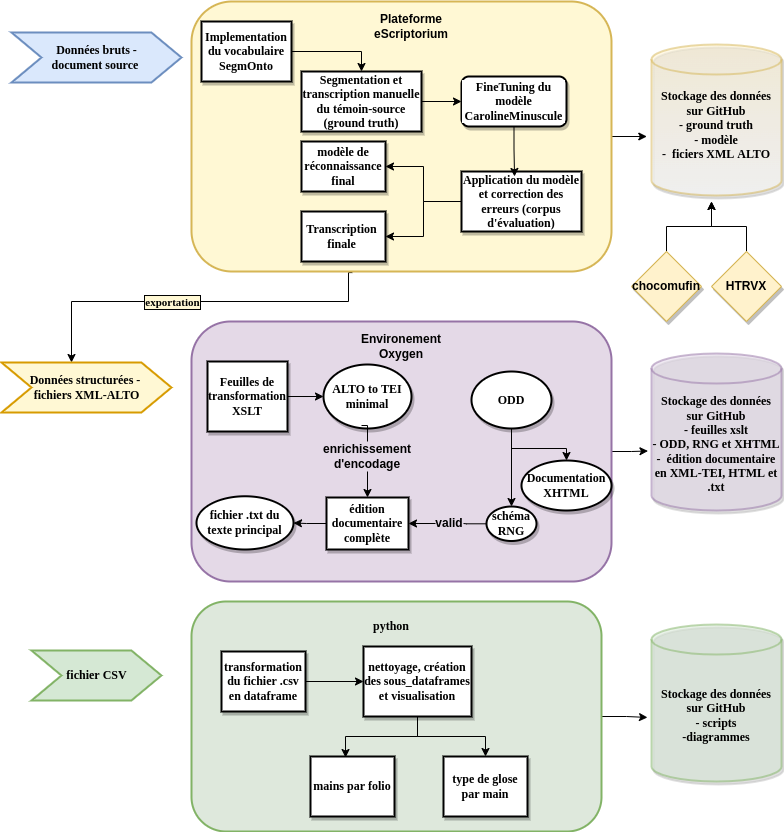
\includegraphics[width=18cm, height=17cm, width=17cm]{pipeline/modelisation_pipeline.png}
    \caption{Modélisation du pipeline suivi. Trois niveaux de traitement successifs, de la transcription à la structuration et la visualisation des données.}
\end{figure}

Le \textit{pipeline} suivant a été conçu en prenant en compte tous les aspects dont : les besoins, les objectifs, les outils, les enjeux techniques, le type d’analyse sur textes extraits et  les résultats attendus. Idéalement, l'objectif de ce projet est le développement d'un pipeline englobant qui prend en compte les spécificités de tous nos témoins, tout en restant souple pour pouvoir être repris par d'qutres projets dans le cadre d'interoperabilité, afin de faciliter l'analyse et l'édition des manuscrits glosés.

\section{Volet 1: Aquisition des données : HTR}

Il existe un large éventail de logiciels d'OCR (Reconnaissance Optique de Caractères) et d'HTR (Reconnaissance automatique de structure et d’écriture manuscrite). Ces logiciels sont utilisés pour convertir des textes imprimés ou manuscrits en format numérique, en les transcrivant automatiquement ou avec une intervention humaine minimale.Certains sont propriétaires et d'autres sont gratuits, et ils ont tous des spécificités qui les rendent plus adaptés à un projet plutôt qu'à un autre. En ce qui concerne le logiciel utilisé pour le projet Eutychès, nous avons opté pour \textit{kraken} \footnote{ \url{https://kraken.re/master/index.html}}, accessible via son interface \textit{eScriptorium}\footnote{\cite{kiessling2019escriptorium}}. Il s'agit d'un outil d’analyse de mise en page et de Reconnaissance Automatique de Structure et d’Écriture manuscrite (HTR) basé sur l'apprentissage profond. Ce choix repose sur deux raisons principales. Premièrement, \textit{kraken} est un logiciel libre disposant d'une documentation étendue, qu'il s'agisse de tutoriels en ligne ou de la documentation présente dans leur \href{https://gitlab.inria.fr/scripta/escriptorium}{dépôt GitLab}. Deuxièmement, les chercheurs de l'ENC et d'Inria ont travaillé activement et en profondeur sur plusieurs projets utilisant \textit{kraken} et eScriptorium. Cela nous a grandement facilité la résolution des problèmes rencontrés tout au long de notre recherche, qu'ils soient d'ordre technique ou méthodologique.

\subsection{Analyse de la mise en page complexe / Complex Layout Analysis}

La première étape de l'acquisition de nos données, dans notre cas les différentes couches de texte présentes dans la copie numérique des folios de nos témoins, consiste en leur segmentation. La segmentation est le processus de découpage de l'image complète en sous-parties pour un traitement ultérieur. Dans notre jeu de données, la segmentation de l'image est effectuée selon l'ordre suivant : segmentation au niveau de la zone, puis segmentation au niveau de la ligne. \\ 


\textit{Kraken} propose déjà un modèle par défaut pour la segmentation des pages écrites de gauche à droite, qui a été entraîné sur un vaste ensemble de données et qui fonctionne assez bien pour les lignes principales de la page, à condition que la qualité de l'image soit bonne. Pendant les deux ans d'élaboration de ce projet, le modèle par défaut a beaucoup amélioré, cependant, compte tenu des spécificités mentionnées précédemment et de l'hétérogénéité significative de la mise en page, le modèle intégré de segmentation de la page n'était pas capable de gérer dans tous les cas la complexité inattendue des informations, telle que la présence de plusieurs lignes interlinéaires ou marginales écrites en petits caractères.\\


\begin{figure}[H]
    \centering
    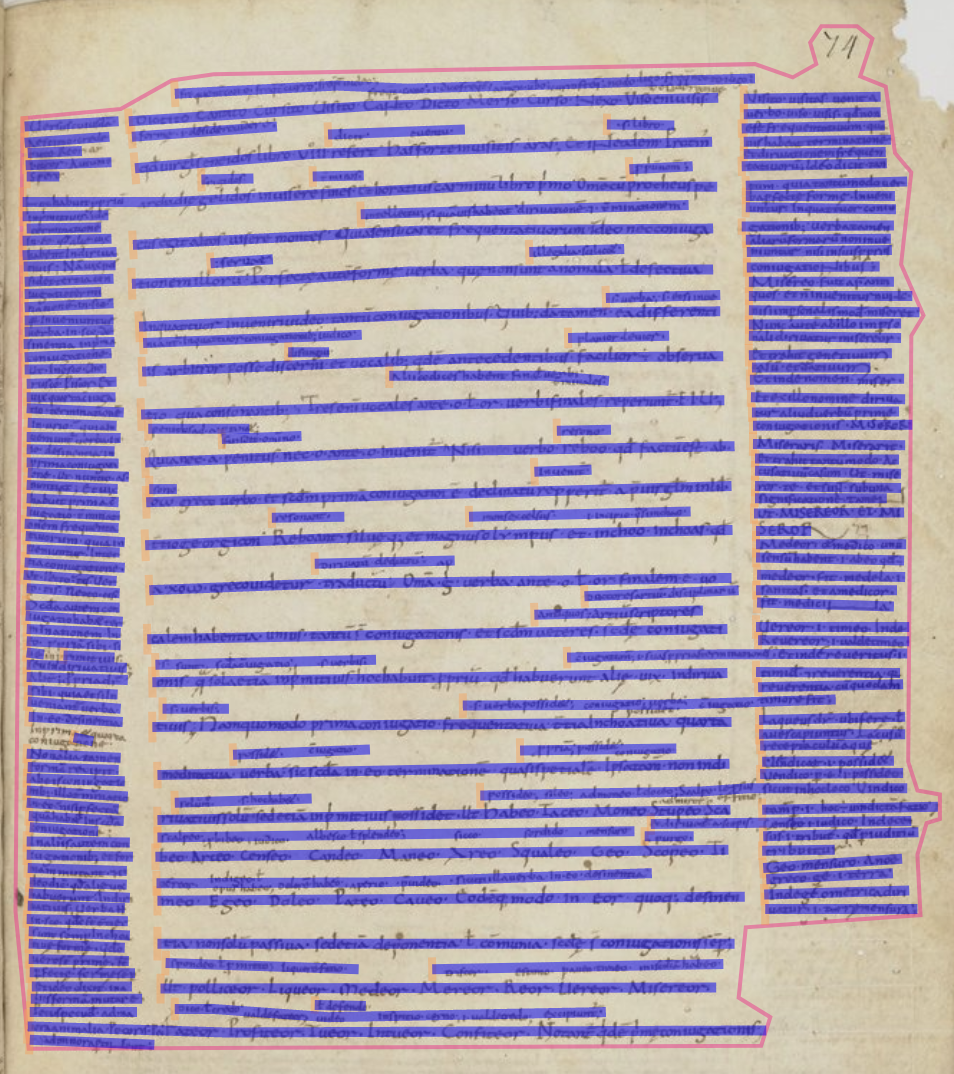
\includegraphics[width=10cm, height=13cm]{segmentation_imgs/segmentation_default_kraken.png}
    \caption{Example de segmentation avec le modèle par défaut de mise en page de \textit{kraken} sur le folio 74r du manuscrit Lat 7499.}
\end{figure}

En réalité, la segmentation des manuscrits glosés va bien au-delà de la simple détection des lignes et des zones. Lors du processus de segmentation, il est essentiel de faire la distinction entre les différentes hiérarchies, que ce soit pour les zones (principales, marginales) ou pour les lignes (principales, interlinéaires). Par conséquent, une approche plus ciblée a été nécessaire afin de prendre en compte ces spécificités et d'effectuer une segmentation adéquate où éventuellement, il s'agit de différencier les niveaux sémantiques distincts qui coexistent dans une image. Prenons l'exemple d'application le plus manifeste : Considérant qu'\textit{eScriptorium} fait une lecture horizontale les lignes en allant de gauche à droite, les colonnes (en marge ou à l'intérieur du texte principal), introduisant une lecture verticale, sont ignorées \footnote{Et pour citer M  Vidal-Gorène dans un récent entretien pour BULAC (cf. supra n.9) : \og{} Ainsi pourrais-je obtenir un CER* de 0\%, mais si les lignes ne sont pas lues dans le bon ordre, est-ce pour autant utile ?\fg{}}.\\

Dans ce cadre, afin de gérer la \textit{Complex Layout Analysis} la stratégie suivante a été mise en place : Avec la perspective de construire un jeu de données pour entraîner un modèle de segmentation nous avons manuellement corrigé la sortie du modèle (étape de post-correction) tout en implémentant un vocabulaire contrôlé pour la description paléographique de l'image. En pratique, la caractérisation des zones et des lignes est très adaptée au cas des manuscrits glosés, étant donnée les doubles contraintes de la mise en page où l'ordre de lecture est perturbé, et les trois niveaux d'information que l'ajout des gloses impose.\\ 

\textsc{SegmOnto}

Un vocabulaire contrôlé est un lexique dont le but est de permettre l'organisation des connaissances pour faciliter la recherche d'informations. Il est utilisé dans les schémas d'indexation par sujet, les thésaurus et les taxonomies, et nécessite l'utilisation de termes préétablis sélectionnés par le concepteur du vocabulaire. Pour identifier les différentes zones du document, le type de lignes présentes sur la page et les caractériser d'un point de vue codicologique, nous avons décidé de mettre en œuvre le vocabulaire contrôlé SegmOnto \footnote{\cite{gabay2021segmonto}}. SegmOnto est né du besoin d'une application informatique de disposer d'un vocabulaire commun limité et d'une ontologie basée sur les normes existantes pour décrire et analyser la mise en page des documents, allant de la catégorisation du contenu à la reconnaissance de texte. SegmOnto se concentre principalement sur le cas des manuscrits, ce qui facilite davantage son utilisation. Cette pratique répond aux besoins croissants dans le domaine de la Reconnaissance Automatique de Structure et d'Écriture manuscrite (HTR). En effet, avec l'émergence d'outils d'analyse de mise en page efficaces et d'interfaces conviviales, le besoin de modèles de segmentation performants augmente, tout comme la nécessité de disposer de grandes quantités de données provenant de l'agrégation de documents des projets différents. Pour cela, les chercheurs doivent s'accorder sur un vocabulaire commun limité et partager des pratiques communes pour favoriser l'interopérabilité de leurs résultats. En adhérant à ce cadre scientifique et en reconnaissant les avantages d'une méthode de description dotée d'une empreinte numérique compatible avec le format ALTO pour les documents à plusieurs niveaux, nous avons implémenté SegmOnto pour l'ensemble de notre jeu de données.\\

Par conséquent, tracer manuellement les différentes \og{} zones de lecture \fg{} avec SegmOnto est une condition indispensable. La page se divise ainsi dans les zones suivantes selon l'information qu'elles portent:

\begin{itemize}
    \item \textit{NumberingZone} pour la foliotation ;
    \item \textit{MainZone}, ou éventuellement \textit{MainZone} pour la zone qui comporte le texte principale ainsi que les gloses interlinéaires;
    \item \textit{MarginTextZone} pour les \textit{marginalia};
    \item \textit{MusicZone} pour les neumes (présents uniquement dans le VLO41) ;
    \item \textit{GraphicZone} pour les dessins (également, uniquement présents dans le VLO41).
\end{itemize}

Il en va de même pour les deux types de lignes. Grâce à l'utilisation de \textit{SegmOnto}, nous sommes en mesure de distinguer et de caractériser les deux niveaux d'information : les lignes principales (marquées en tant que \textit{DefaultLine}) et les interlignes (marquées en tant qu'\textit{InterlinearLines}) et pour le cas du BambergMsc30 nous avons caractérisé les gloses tironiennes (avec le tag \textit{TironianSignLine}). Cela élimine toute ambiguïté quant à la nature de chaque ligne et facilite l'extraction et l'exploitation des données, offrant ainsi un outil d'indexation tout en facilitant l'extraction et l'exploitation des données. Cette indexation permet une sélection plus fine lors de l'exportation lors de l'exportation de la plate-forme.Nous avons la possibilité d'exporter uniquement le texte principal, la zone principale, les gloses, etc., en fonction du type d'analyse que nous souhaitons effectuer. \\

Des exemples d'indexation des zones et des lignes sont présentés dans la Figure 2.2 ci-dessous. :\\

\begin{figure}[H]
    \begin{subfigure}{0.40\textwidth}
    \centering
    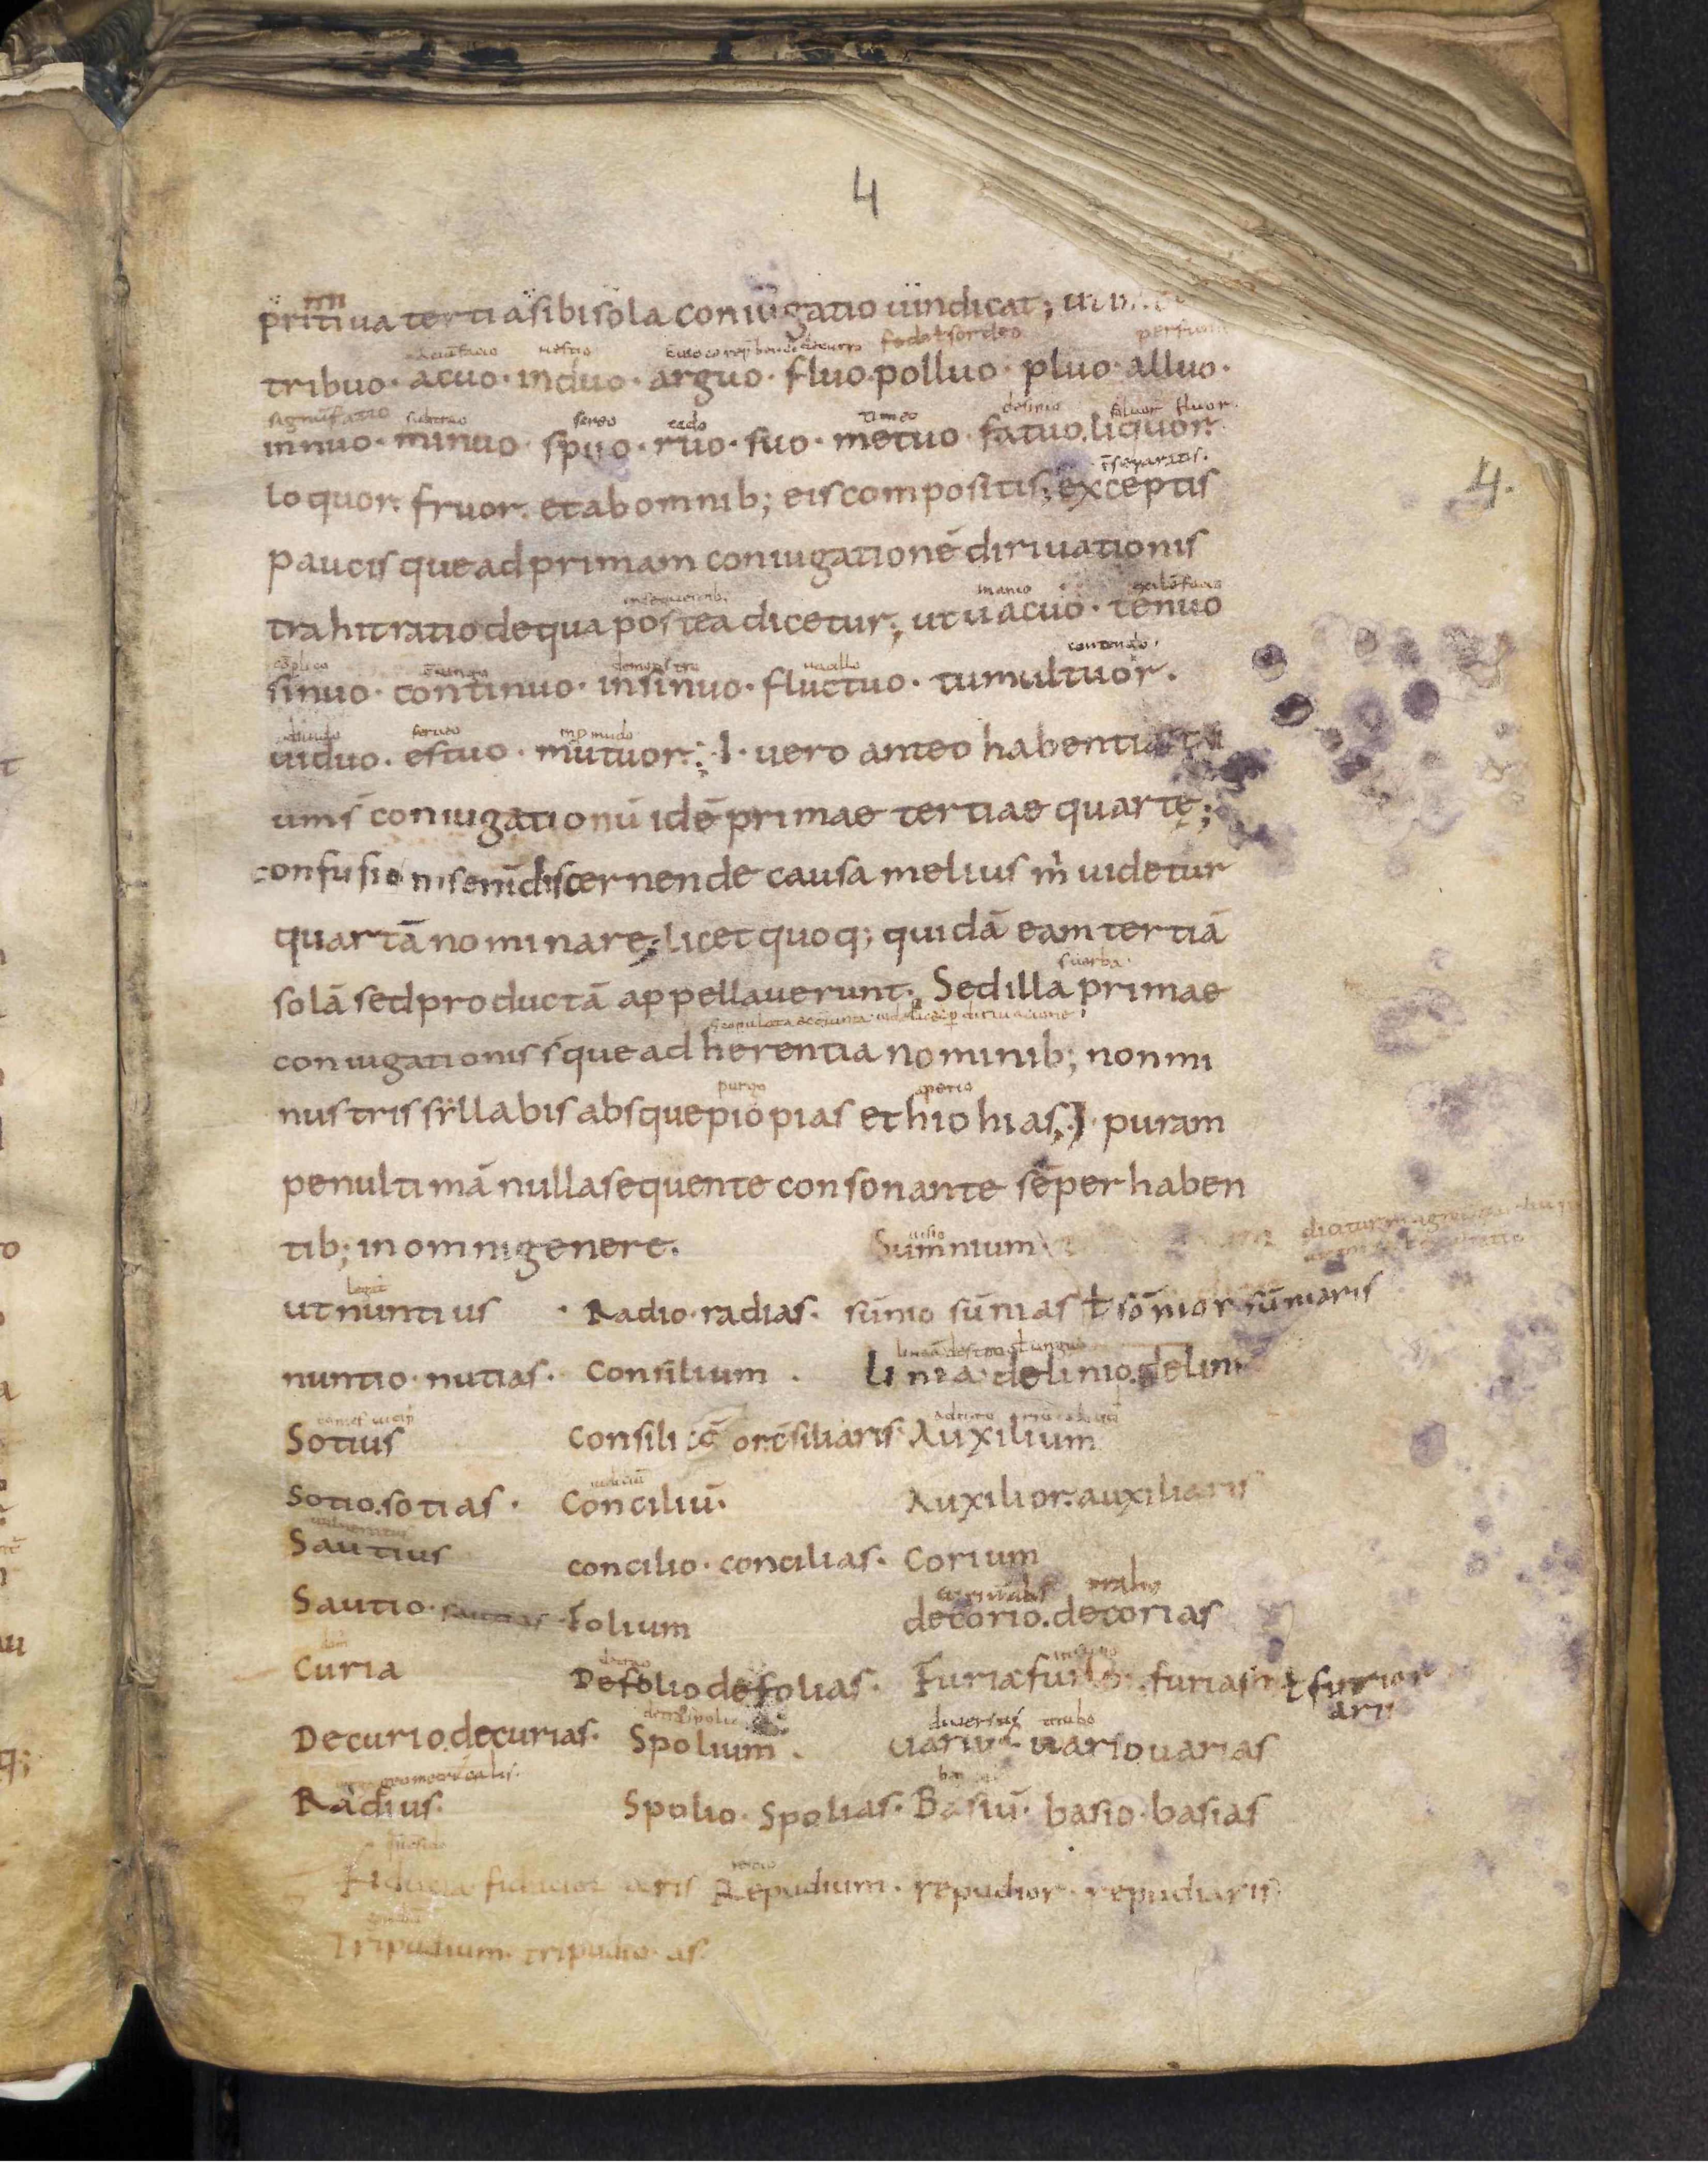
\includegraphics[width=7cm]{segmentation_imgs/4r.png}
    \caption{VLO41 folio 4r}
    \end{subfigure}
    \begin{subfigure}{0,40\linewidth}
    \centering
    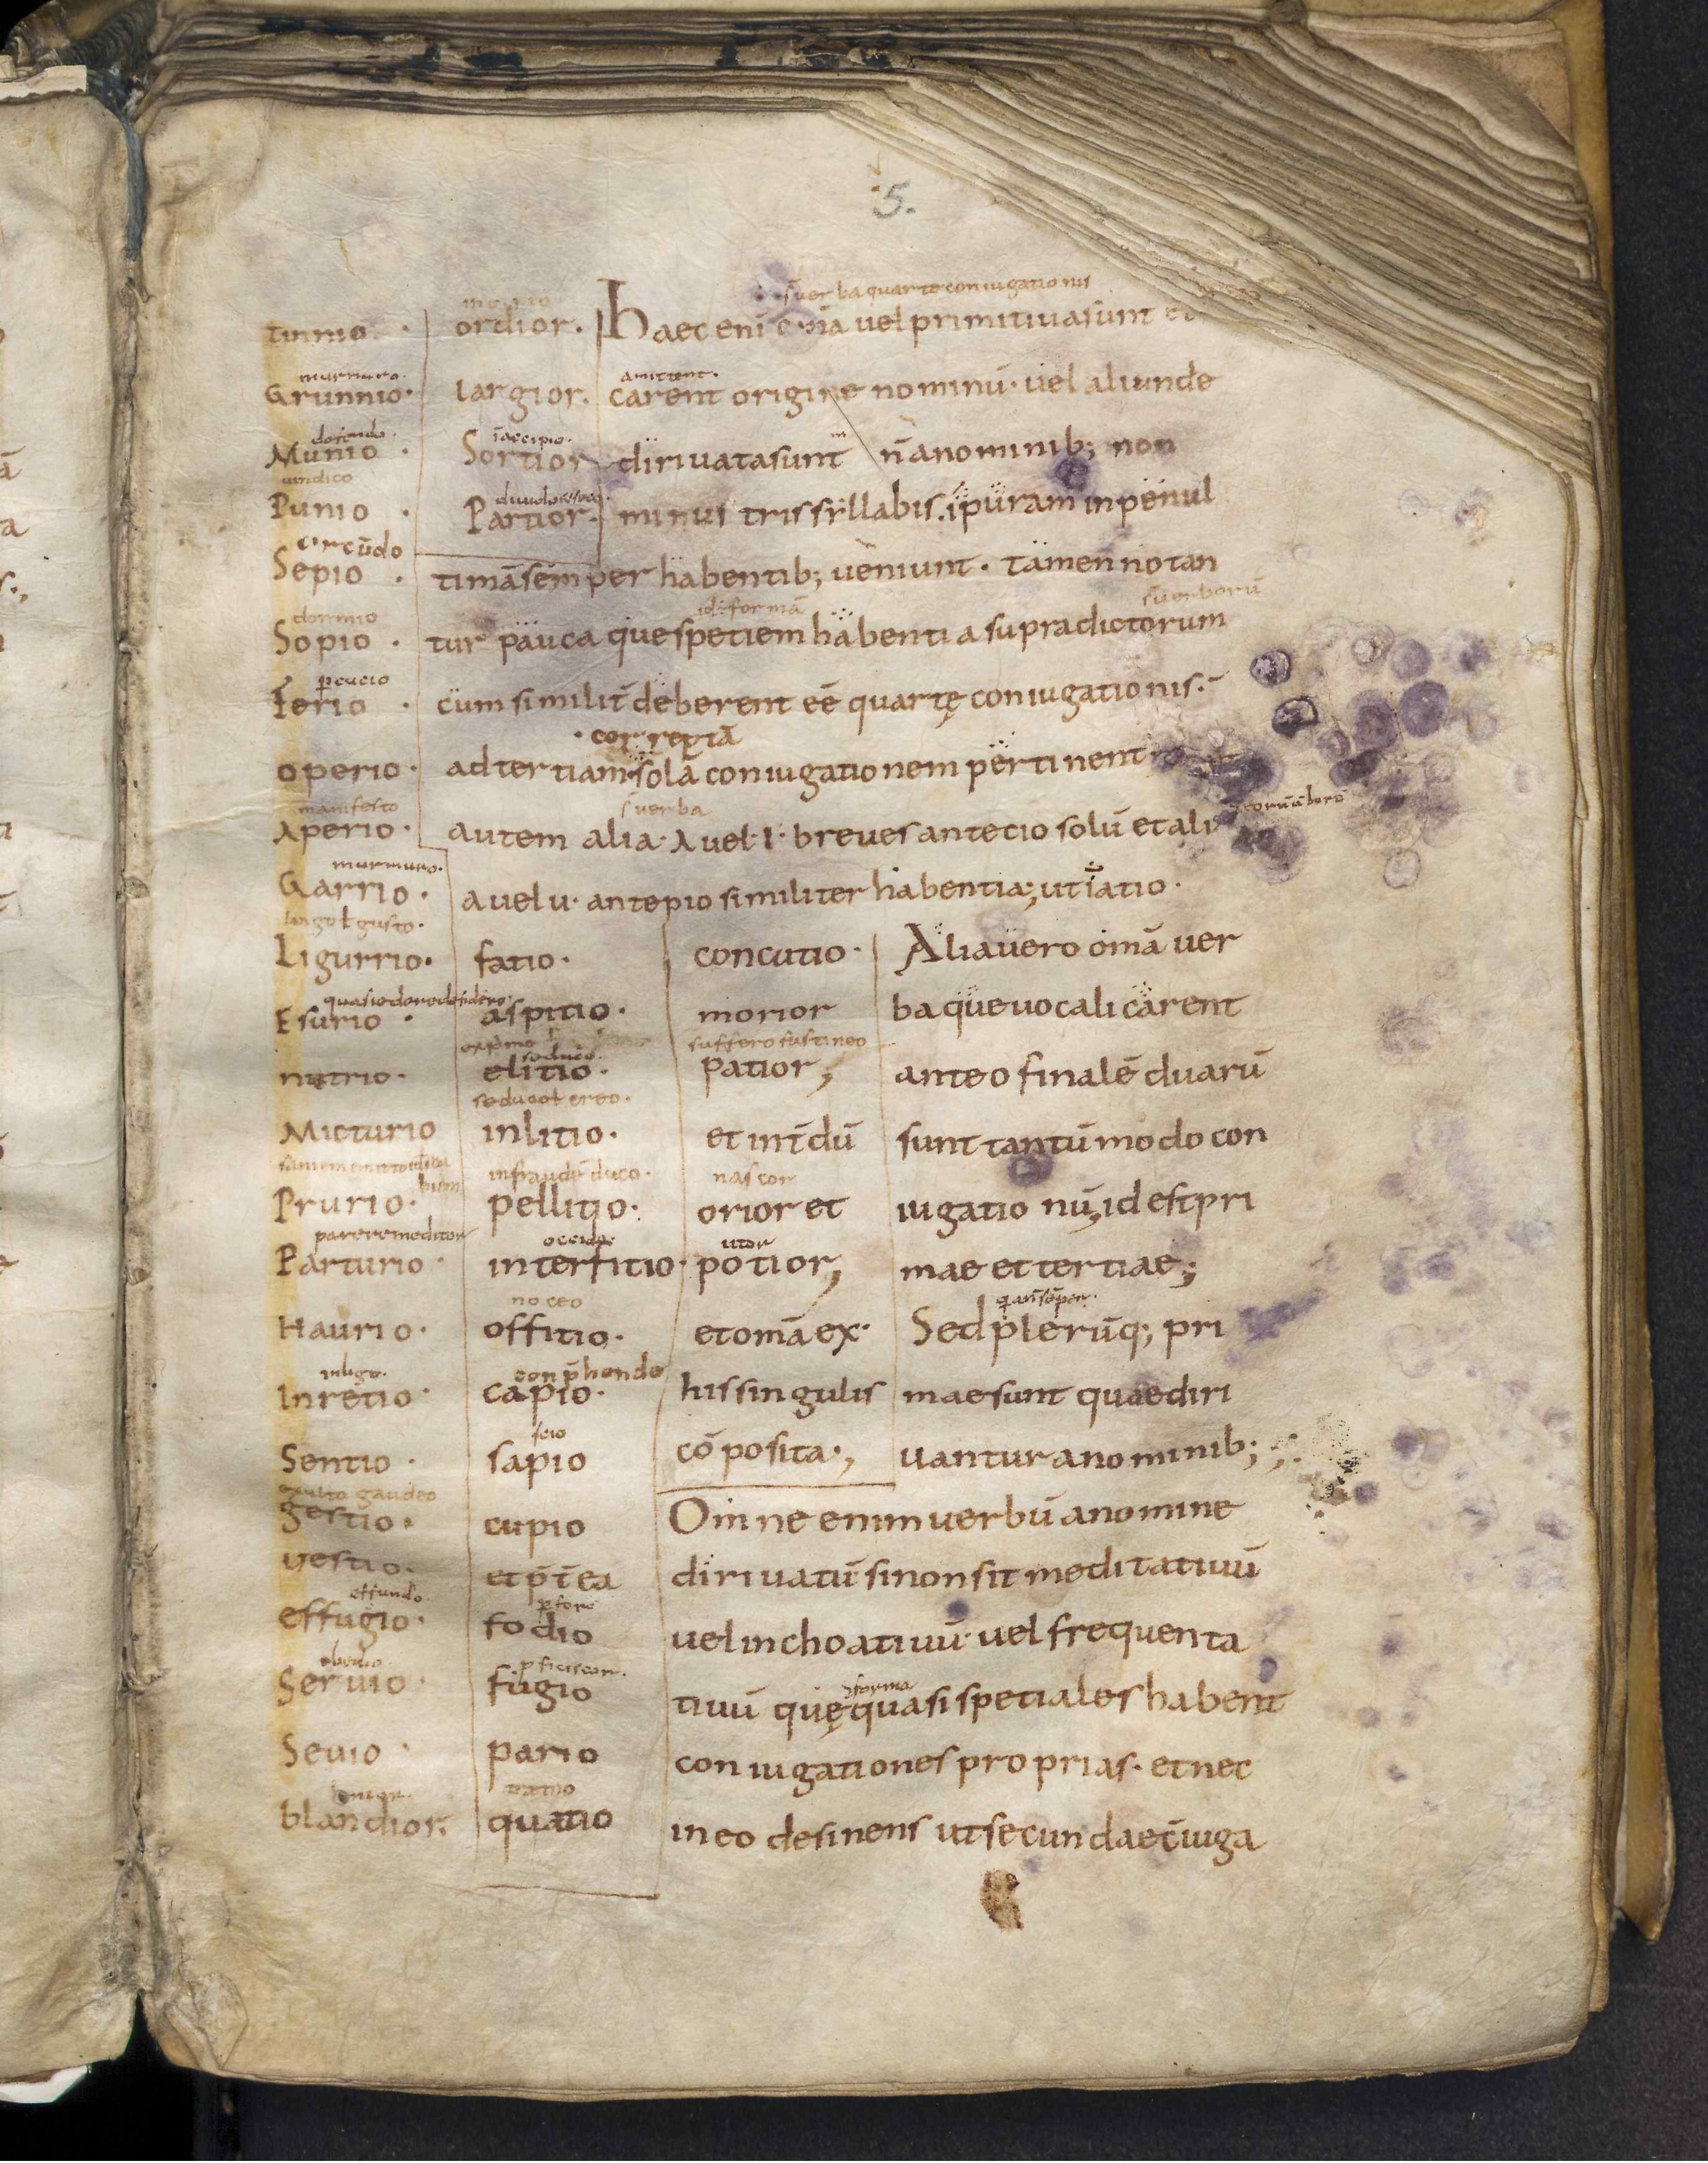
\includegraphics[width=7cm]{segmentation_imgs/5r.png}
    \caption{VLO41 folio 5r}
    \end{subfigure} 
    \begin{subfigure}{0,40\linewidth}
    \centering
\includegraphics[width=8cm, height= 10cm]{segmentation_imgs/segmentation_zone_76r.png}
    \caption{Lat7499 folio 76r }
    \end{subfigure}
     \begin{subfigure}{0,80\linewidth}
    \centering
\includegraphics[width=7cm, height= 10cm]{segmentation_imgs/segmentation_lines_Lat7499_84v.png}
    \caption{Lat7499 folio 84v }
    \end{subfigure}
    \caption{ (a) et (b) Disposition des zones SegmOnto afin de rétablir le sens de lecture. (c) Mise en page standard avec MainZone et MarginTextZone (d) DefaultLines en rose InterlinearLines en bleu}
\end{figure} 




\subsubsection{Description du jeu des données pour la segmentation}

La création d'un jeu de données, y compris la segmentation et la transcription, et en particulier d'un jeu de données composé de manuscrits glosés, peut être un processus très chronophage et fastidieux. D'ailleurs, la rareté et la difficulté d'accès aux données annotées manuellement sont souvent discutées, notamment pour des tâches comme la Complex Layout Analysis. C'est pourquoi il est nécessaire de disposer d'une vérité de terrain disponible en accès libre et de créer des modèles qui peuvent être appliqués pour faciliter ce processus. L'un des objectifs de ce projet est de produire à la fois une vérité de terrain conséquente et la publication d'un modèle de segmentation en accès libre destiné à la communauté des chercheurs qui souhaitent traiter numériquement leurs manuscrits glosés en tirant parti du travail précédent.\\

Quant à notre jeu de données original, il comprend 4 manuscrits et un total de 135 pages, dont 3/4 sont glosées à différents degrés. Malheureusement, cette quantité n'est pas suffisante pour la tâche complexe que nous souhaitons accomplir : entraîner un modèle capable de détecter et de classer automatiquement les deux types de zones et de lignes. Pour cette raison, nous sommes obligés d'augmenter la taille de notre vérité de terrain. Heureusement pour notre projet, un deuxième jeu de données de manuscrits glosés est disponible en accès libre, à savoir le jeu de données Diva-HisDB\footnote{\url{https://paperswithcode.com/paper/diva-hisdb-a-precisely-annotated-large}}, créé par l'équipe Document, Image and Voice Analysis Group (DIVA) de l'Université de Fribourg, destiné à l'évaluation de plusieurs tâches d'analyse d'images de documents (DIA)\footnote{L'équipe a publié des recherches dans le domaine de Complex Layout Analysis (\cite{simistira2016diva}) et récemment a développé un framework pour la segmentation sémantique des Complax Layout Analysis qui fait usage des autoencodeurs : \cite{vogtlin2022diva}}. La vérité de terrain comprend 150 pages de manuscrits segmentés au niveau des pixels \footnote{sc. Pixel-wise semantic segmentation où chaque pixel est classé soit en tant que \og{}Text\fg{} soit en tant que \og{}Commentaire\fg{}} avec une précision extraordinaire, au format PAGE,uniquement récemment dotés de baselines que nous avons pu repérer, adapter et intégrer dans notre jeu de données. L'adaptation consiste en une annotation manuelle des documents avec notre ontologie \textit{SegmOnto}. Pour ce qui est de plus, les typologies représentées par les manuscrits en question correspondent à 100\% à nos typologies, cf la figure ci-dessous: 


\begin{figure}[H]
  \centering
 {\includegraphics[width=12cm,height=5cm]{segmentation_imgs/DivaHisDB/apercu_DIVA.png}}
  \qquad
  {\includegraphics[width=12cm,height=5cm]{segmentation_imgs/DivaHisDB/segmentation_DIVA.png}}
  \caption{Exemples des typologies et les polygons de segmentation du dataset DIVAHisDB. Classe \og{}Texte\fg{} en bleu classe \og{}Commentaires\fg{} en vert.}
  \label{fig:my_figure}
\end{figure}


L'ajout de ces 3 manuscrits déjà segmentés avec une résolution excellente et des polygones très précis autour des lignes a été crucial pour cette étape d'entraînement et pour l'efficacité du modèle qui en résulte. Voici la composition de notre nouveau jeu de données destinée à la l'entraînement d'un modèle de segmentation:

\begin{table}[H]
\centering
\resizebox{\textwidth}{!}{%
\begin{tabular}{|c|c|c|c|c|c|c|}
\hline
\rowcolor{gray!25}
\textbf{Cote} & \textbf{Pages} & \textbf{MainZones} & \textbf{MarginTextZones} & \textbf{NumberingZones} & \textbf{DefaultLines} & \textbf{InterlinearLines} \\
\hline
% Row 1
VLO41 & 63 & 78 & 51 & 32 & 1768 & 973 \\
\hline
% Row 2
BambergMsc30 & 30 & 30 & 167 & 15 & 1748 & 1590 \\
\hline
Lat7499 & 39 & 39 & 79 & 18 & 3900 & 2207 \\
\hline
CSG863 & 40 & 40 & 87 & 41 & 1911 & 278 \\
\hline
CGS18 & 40 & 40 & 283 & 34 & 4648 & 1360 \\
\hline
CB55 & 48 & 49 & 176 & 13 & 3106 & 0 \\
\hline
\hline
\rowcolor{gray!25}
\textbf{Total} & \textbf{260} & \textbf{276} & \textbf{843} & \textbf{153} & \textbf{17081} & \textbf{6408} \\
\hline
\end{tabular}%
}
\caption{Jeu de données pour l'entraînement des modèle de segmentation sémantique YALTAi - kraken}
\label{tab:dataset_segmentation}
\end{table}



Biais du jeu de données pour l'entraînement : il est important de noter qu'il existe un biais dans le jeu de données, que l'utilisateur du modèle ou de la vérité de terrain doit garder à l'esprit. En raison de la typologie spécifique de notre dataset, le modèle sera plus efficace lorsqu'il est appliqué aux manuscrits présentant une disposition hiérarchique du contenu, avec le texte principal en bloc au milieu de la page et accompagné de gloses interlinéaires. En ce qui concerne les marginalia, on observe un degré de densité différent, avec des lignes éparses, de petits blocs de texte ou même des paragraphes entiers en marge.\\


\begin{figure}[H]
    \centering
    \includegraphics[height=13cm, width=15cm]{modelisation_graphs/Holtz_Powitz_typologyXIe_classe A.jpg}
    \caption{La diversité des typologies codifié par Powitz/Holtz pour les commentaires entre le \textsc{viii}\ieme{} et le \textsc{xi}\ieme{}. Notre typologie est entre P3 et P10.}
    \label{typologies}
\end{figure}

\subsubsection{Segmentation avec kraken}

L'extraction automatique de texte est désormais une activité essentielle en philologie numérique, comme en témoignent les récentes compétitions ICDAR, et dans la création de corpus pour les documents historiques. En ce qui concerne l'architecture \textit{Kraken}, utilisée par \textit{eScriptorium}, elle offre la possibilité d'entraîner des modèles de segmentation sémantique, ce qui est un aspect essentiel de notre approche de création de données. Cependant, notre expérience dans la formation d'un tel modèle n'a pas donné les résultats escomptés, en raison de la complexité élevée de la tâche et de la quantité insuffisante de notre jeu de données, qui a été segmenté et annoté manuellement. Le modèle obtenu après l'entraînement de l'ensemble de notre jeu de données, bien qu'il attribue en principe correctement les classes aux zones/lignes correspondantes, nécessite un post-traitement conséquent (cf.\ref{segmentation-kraken})pour obtenir les résultats souhaités. Malheureusement, il ne parvient pas pour l'instant à atteindre notre objectif de réduire au maximum la tâche de production et d'annotation des données, et nous ne pouvons que être d'accord avec Thibault Clérice\footnote{\cite{clerice2022YALTAi},p.1} que \quote{ [...]Kraken [...]has suffered from poor performances user-perception, specifically with small dataset (around a thousand sample for train/dev/test) or very small dataset (less than 300 for train and dev). This results perception has slowed the improvement of automatic information extraction[...]. If the segmenter is not able to recognize columns (or separate them) in medieval manuscripts or does not distinguish main bodies of text from foot
notes, the co-occurrences of the extracted text are fooled by a wrong interpretation of the layout.}

\begin{figure}[H]
    \centering
    \begin{subfigure}[b]{0.5\textwidth}
        \centering
        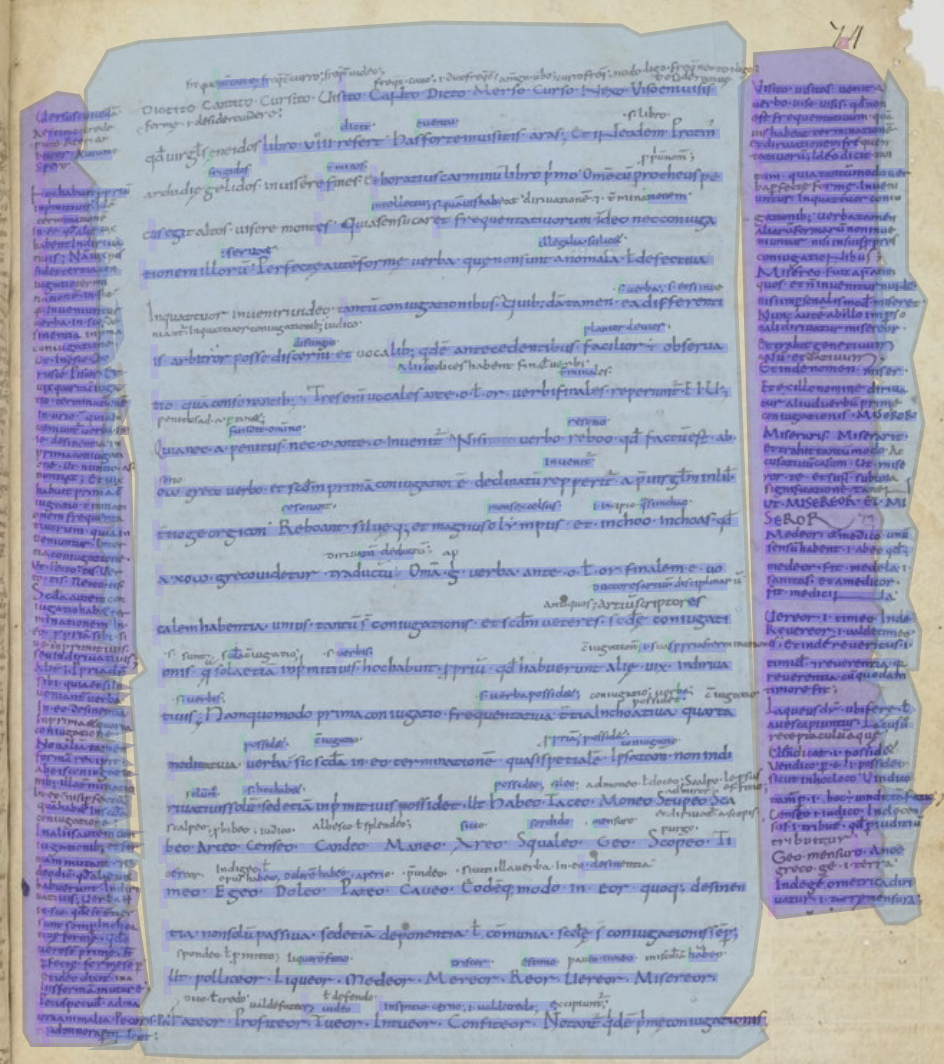
\includegraphics[width=7cm, height=9cm]{segmentation_imgs/segmentation-zones-kraken-model-Eutyches.png}
        \label{fig:sub1}
    \end{subfigure}%
    \begin{subfigure}[b]{0.5\textwidth}
        \centering
        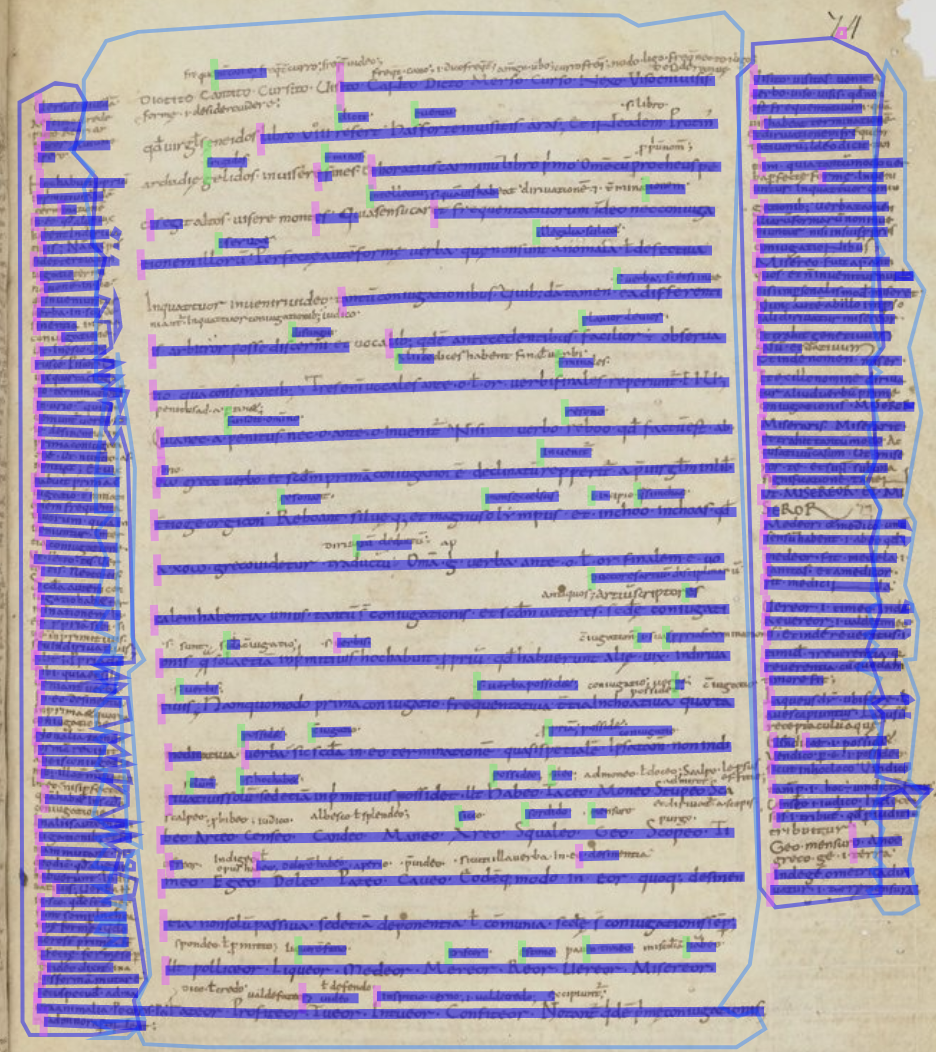
\includegraphics[width=7cm, height=9cm]{segmentation_imgs/segmentation-lines-kraken-model-Eutyches.png}
        \label{fig:sub2}
    \end{subfigure}
    \caption{Résultats qualitatifs du modèle de segmentation sémantique des zones/lignes kraken entraîné sur l'ensemble de nos données. Plusieurs lignes manquées ou/et coupées, mal-classées.}
    \label{segmentation-kraken}
\end{figure}



\subsubsection{Segmentation des zones/lignes avec YALTAi-kraken}

La différence entre l'approche de la \textit{bounding box} et la détection par polygone, ainsi que la catégorisation des pixels, réside dans la manière dont la segmentation sémantique est effectuée. Dans l'approche de la \textit{bounding box}, on utilise des rectangles isothétiques pour encadrer les zones d'intérêt, ce qui permet de délimiter grossièrement les régions du document sans se soucier de la forme précise de ces régions. Cela offre une certaine simplicité dans l'annotation et la manipulation des zones, mais peut ne pas être suffisamment précis pour certains cas, en particulier lorsque les formes des zones sont complexes ou irrégulières. Pour notre jeu de données spécifique, la plupart des classes de zones sont bien délimitées, avec peu de superpositions entre le texte principal et les \textit{marginalia}. \\

La détection par polygone consiste à utiliser des polygones pour représenter les contours exacts des zones. Cela permet une segmentation plus précise, car les polygones peuvent représenter les contours des régions d'intérêt de manière plus fidèle. Cette approche est la plus pertinente pour la gestion des lignes, car les lignes ne peuvent pas être réduites à des rectangles plus grossiers en raison de la disposition verticale des lignes principales et des interlignes, ce qui pourrait nuire à la tâche suivante, celle de reconnaissance des caractères.
Par contre, Lorsqu'on utilise la catégorisation des pixels, chaque pixel est attribué à une classe ou une catégorie spécifique, mais cela ne tient pas compte de la structure hiérarchique des zones et des lignes dans le document.En d'autres termes, la catégorisation des pixels ne permet pas de déterminer comment les pixels doivent être regroupés pour former des zones distinctes, ni comment les zones doivent être organisées pour contenir des lignes et du contenu. Cela peut entraîner des résultats moins cohérents ou pertinents pour la segmentation sémantique, car la structure globale du document n'est pas prise en compte.\\

Les avantages et les inconvénients des différentes approches peuvent varier en fonction du contexte spécifique et des exigences de la tâche de segmentation sémantique. Les désavantages de la catégorisation des pixels ou de la détection par polygone pour la segmentation des zones dans les documents historiques résident dans la complexité et l'irrégularité des formes présentes dans ces documents. Les documents historiques peuvent contenir des mises en page complexes, des formes irrégulières, des variations de taille et de forme des zones, des superpositions de texte, etc. Les approches basées sur les pixels ou les polygones peuvent avoir du mal à capturer avec précision ces caractéristiques complexes, ce qui peut entraîner des erreurs de segmentation ou une perte de détails importants. Certains travaux de recherche se concentrent sur le développement de méthodes combinant ces approches afin de tirer parti de leurs forces respectives et de surmonter leurs limitations. Un exemple notable de ces approches est YALTAi (You Actually Look Twice at it)\footnote{\url{https://github.com/PonteIneptique/YALTAi/tree/main}}
, développé par Thibault Clérice en 2022, qui combine la détection d'objets avec YOLOv5 \footnote{YOLO est un logiciel de semantic segmentation \cite{yolo_glenn_jocher_2022_7347926}: Semantic segmentation vise à attribuer une étiquette sémantique à chaque pixel de l'image, en les regroupant en classes prédéfinies. L'objectif est de comprendre la structure et la signification de l'image en termes de catégories d'objets.} pour les zones et l'approche par défaut de Kraken pour la détection et la classification des lignes. \\
 
En appliquant YALTAi, nous passons de la tâche d'analyse de la mise en page, qui consiste à catégoriser les pixels ou à segmenter les polygones, à une tâche de détection d'objets, où chaque région est une instance d'une catégorie de zone, mélangeant ainsi la segmentation et la classification dans l'analyse de la mise en page. Pour la description de l'outil et ses applications dans des datasets tabulaires et manuscrits voir \cite{clerice2022YALTAi}.\\


Nous avons entraîné avec la totalité de notre dataset (voir \ref{tab:dataset_segmentation}) YALTAI sur un GPU avec une taille de lot (batch size) de 2. Le modèle a été entraîné pendant 50 époques et le meilleur modèle a été sélectionné en fonction du score mAP sur l'ensemble de validation. L'évaluation est basée sur la précision moyenne (mAP) et la précision moyenne (AP). Le mAP est utilisé avec un seuil d'intersection sur union de 0,5 (généralement noté mAP@0.5).  Les résultats quantitatifs obtenus sont très prometteurs (Figure \ref{fig:yaltairesults}).

\begin{figure}[H]
  \centering
  \begin{subfigure}[b]{15cm}
    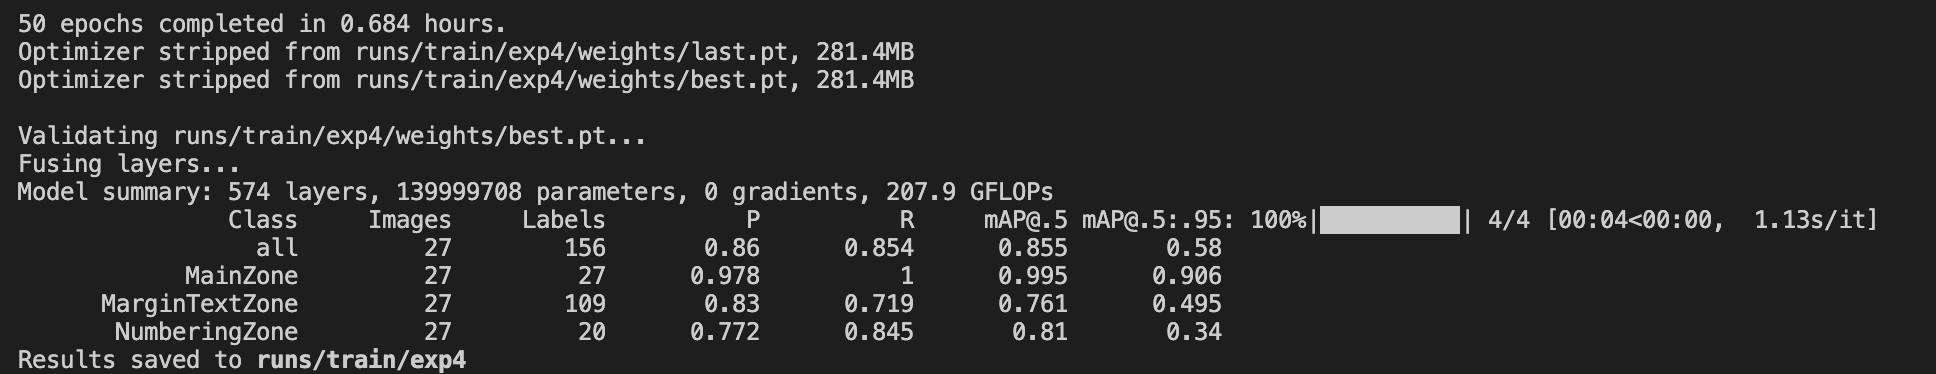
\includegraphics[width=\textwidth,height=3cm]{YALTAi/expe4_3typologies_batch4_epochs50.png}
    \caption{Résultats sur le set d'évaluation}
    \label{fig:subfig1}
  \end{subfigure}
  \vspace{0.5cm}
  
  \begin{subfigure}[b]{15cm}
    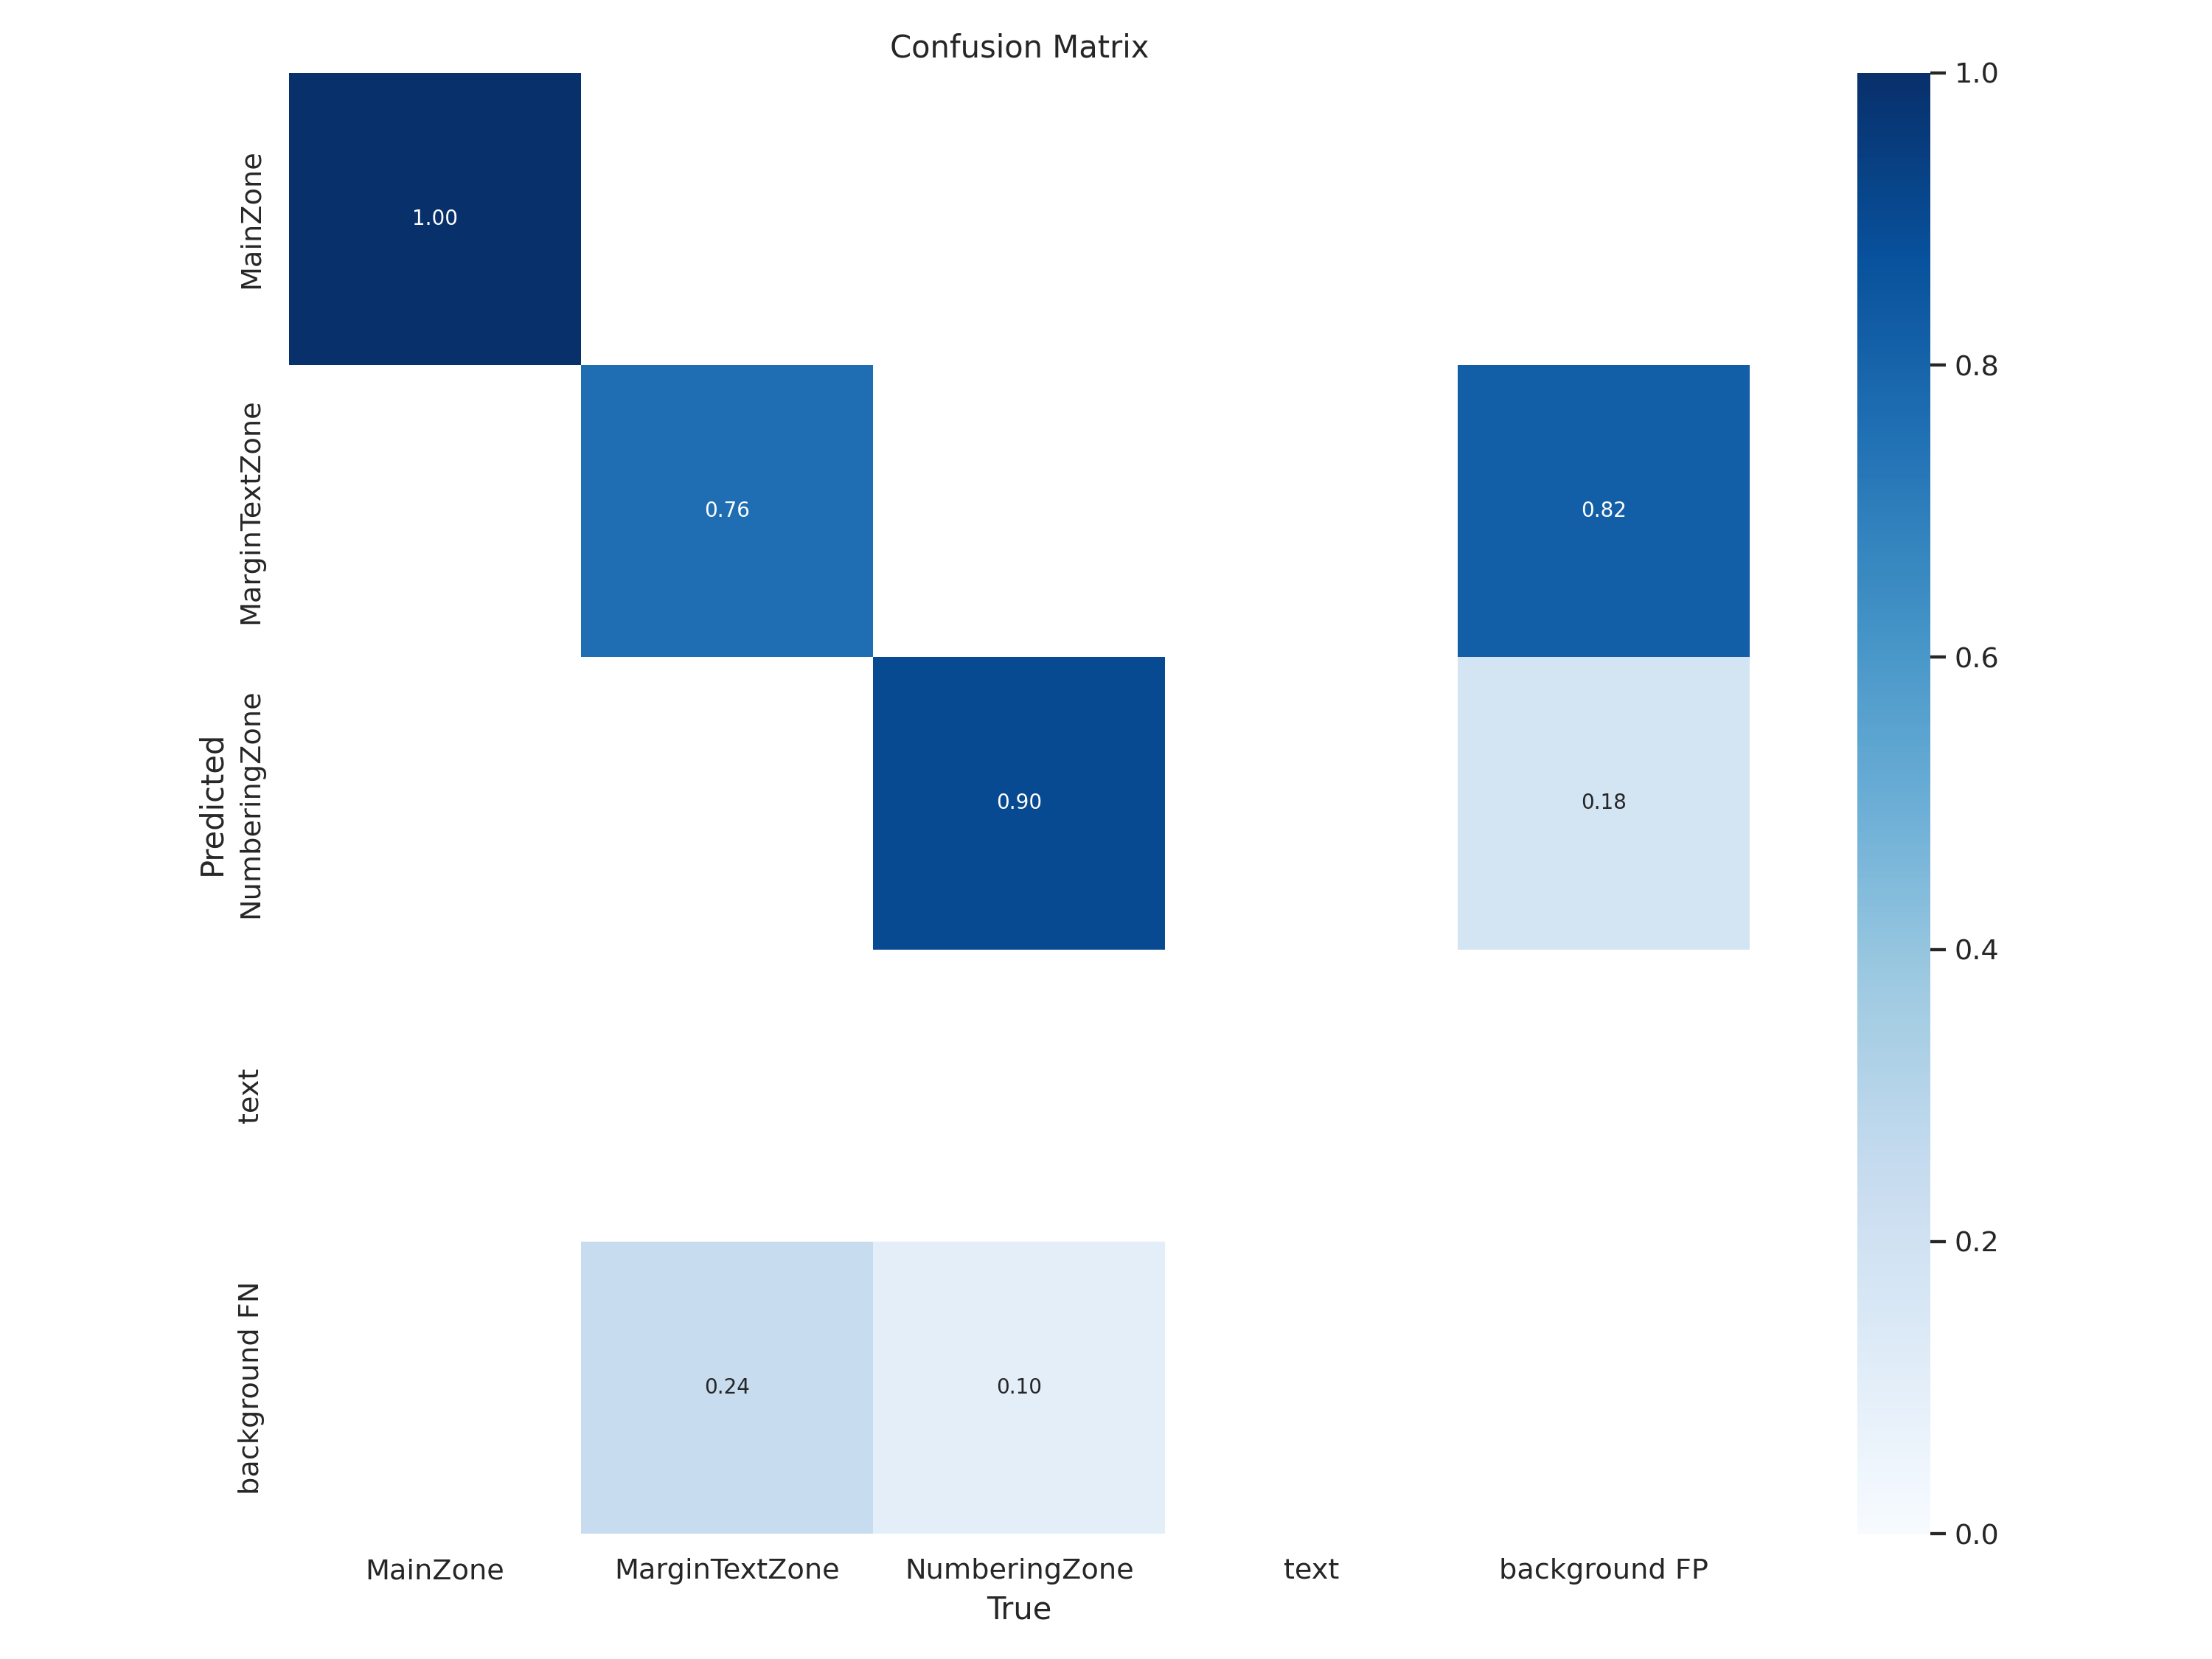
\includegraphics[width=\textwidth,height=11cm]{YALTAi/confusion_matrix.png}
    \caption{Matrice de confusion}
    \label{fig:subfig2}
  \end{subfigure}
  \caption{Résultats quantitatifs du modèle YALTAi sur notre dataset}
  \label{fig:yaltairesults}
\end{figure}

Selon la matrice de confusion générée par YALTAi, l'algorithme a réussi la classification des zones, notamment pour la classe MainZone, où nous obtenons une précision, un rappel, un mAP@.5 et un mAP@5:.95 proches de 1. Cette performance était en grande partie attendue, car il n'y a rien d'imprévisible dans cette classe qui, selon la typologie du jeu de données, est toujours située au milieu de la page. En revanche, la détection et la classification des deux autres classes, à savoir MarginTextZone et NumberingZone, semblent légèrement plus difficiles, car elles sont souvent confondues avec l'arrière-plan (équivalent à l'absence de classe).\\


En termes de logiciel et d'entraînement des modèles, chaque modèle est maintenu indépendant : YOLOv5 est entraîné dans le cadre de YOLOv5, tandis que la segmentation des lignes \textit{kraken} est également entraînée séparément (avec la possibilité d'importer des modèles déjà entraînes, comme nous avons opté dans notre cas). Les deux modèles sont ensuite utilisés ensemble lors de l'inférence/évaluation. Au lieu d'utiliser le modèle de segmentation de baselines par défaut, nous avons entraîné deux modèles distincts -toujours avec la totalité du jeu des données (cf. Figure \ref{tab:dataset_segmentation})-pour les baselines sémantiques/caractérisées : \textit{DefaultLine} et \textit{InterlinearLine}\footnote{L'API de kraken est assez facile à prendre en main grâce à sa documentation étendue \url{https://kraken.re/main/advanced.html\#baseline-segmentation}. Nous voulons remercier également M Vidal-Gorène d'avoir apporté son aide technique à l'entraînement des modèles}. Cette approche vise à offrir la possibilité de traiter et/ou extraire plus facilement des catégories spécifiques comme le texte principal ou les gloses interlinéaires, en fonction des besoins spécifiques du projet \footnote{tous les modèles sont disponibles dans notre \href{https://github.com/malamatenia/Eutyches/tree/main/kraken-YALTAi/models}{dêpot Github}. Les poids du modèle YALTAi, en raison de leur taille, ont dû être stockés dans un \href{https://drive.google.com/drive/folders/1rSgZx_f-bUTKbUeGbbdsMLeJENp4Oj2q?usp=share_link}{GoogleDrive link}.}. Ce qui est pratique avec la plate-forme \textit{eScriptorium}, c'est la possibilité d'appliquer successivement deux modèles de segmentation sans écraser la segmentation précédente, ce qui permet de les combiner si nécessaire. Après avoir importé les modèles entraînés dans la plate-forme, les mesures de performance n'étaient pas aussi élevées que prévu lors de l'entraînement :\\


\begin{figure}[H]
    \centering
    \begin{subfigure}[b]{\textwidth}
        \centering
        \includegraphics[width=\textwidth,height=4cm]{YALTAi/entrainement_kraken_lignes.png}
        \caption{Accuracy et mean\_iu en train et test lors de la dernière époque d'entraînement.}
    \end{subfigure}
    \vskip\baselineskip
    \begin{subfigure}[b]{\textwidth}
        \centering
        \includegraphics[width=\textwidth,height=2cm]{YALTAi/baselines_accuracy.png}
        \caption{Accuracy des modèles Interlinéaire et Default sur eScriptorium.}
    \end{subfigure}
    \caption{Overall figure caption.}
    \label{fig:figure_label}
\end{figure}



Il reste à évaluer la cohérence entre les résultats quantitatifs et qualitatifs. Le modèle a été évalué sur un corpus de test composé d'un témoin tiré de la tradition manuscrite glosée d'Eutychès, à savoir Bodl. MS. Auct. F. 4. 32,  qui présente une typologie similaire à celle de l'ensemble de données d'entraînement.

\begin{figure}[H]
  \centering
  \begin{subfigure}{0.5\textwidth}
    \centering
    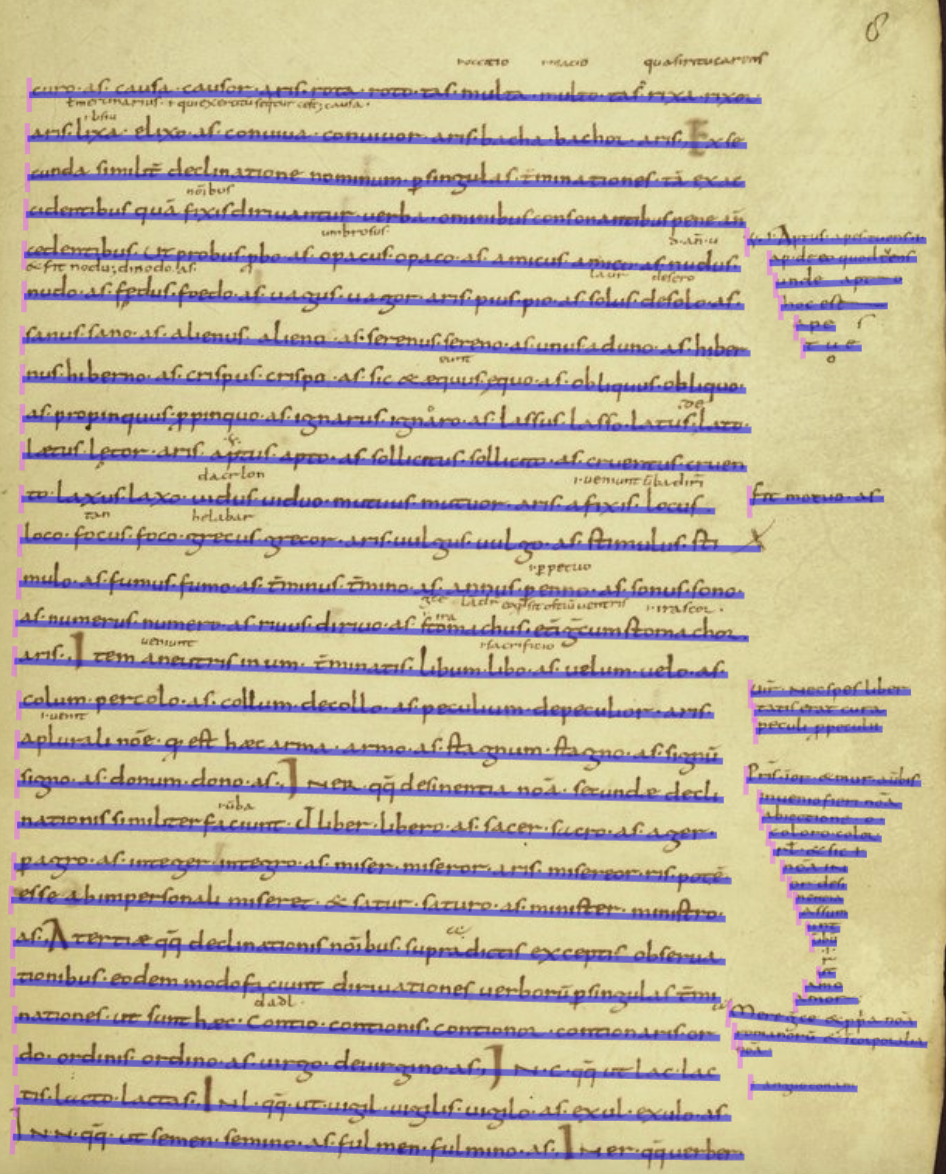
\includegraphics[height=10cm]{YALTAi/test_images/Bodl_Auct.F.4.32.DefaultLine_f08r.png}
    \caption{folio 6r : Application du modèle pour les DefaultLines.}
  \end{subfigure}
  \hspace{1cm} % Adjust the horizontal spacing between the first and second subfigures
  \begin{subfigure}{0.4\textwidth}
    \centering
    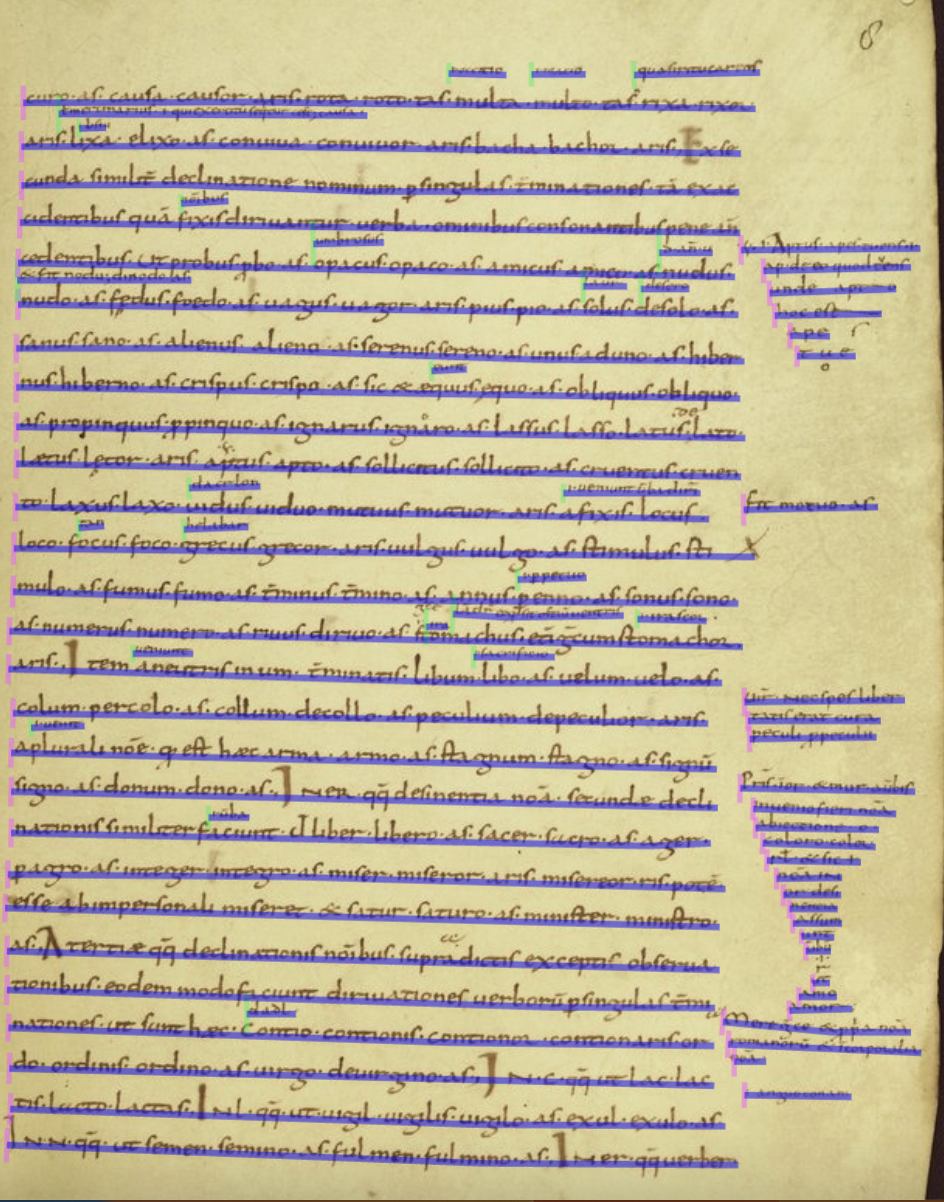
\includegraphics[height=10cm]{YALTAi/test_images/Bodl_Auct.F.4.32.InterlinearLine_f08r.png}
    \caption{folio 6r : Application du modèle pour les InterlinearLines.}
  \end{subfigure}
  
  \vspace{0.5cm} % Adjust the vertical spacing between the top and bottom subfigures
  
  \begin{subfigure}{0.5\textwidth}
    \centering
    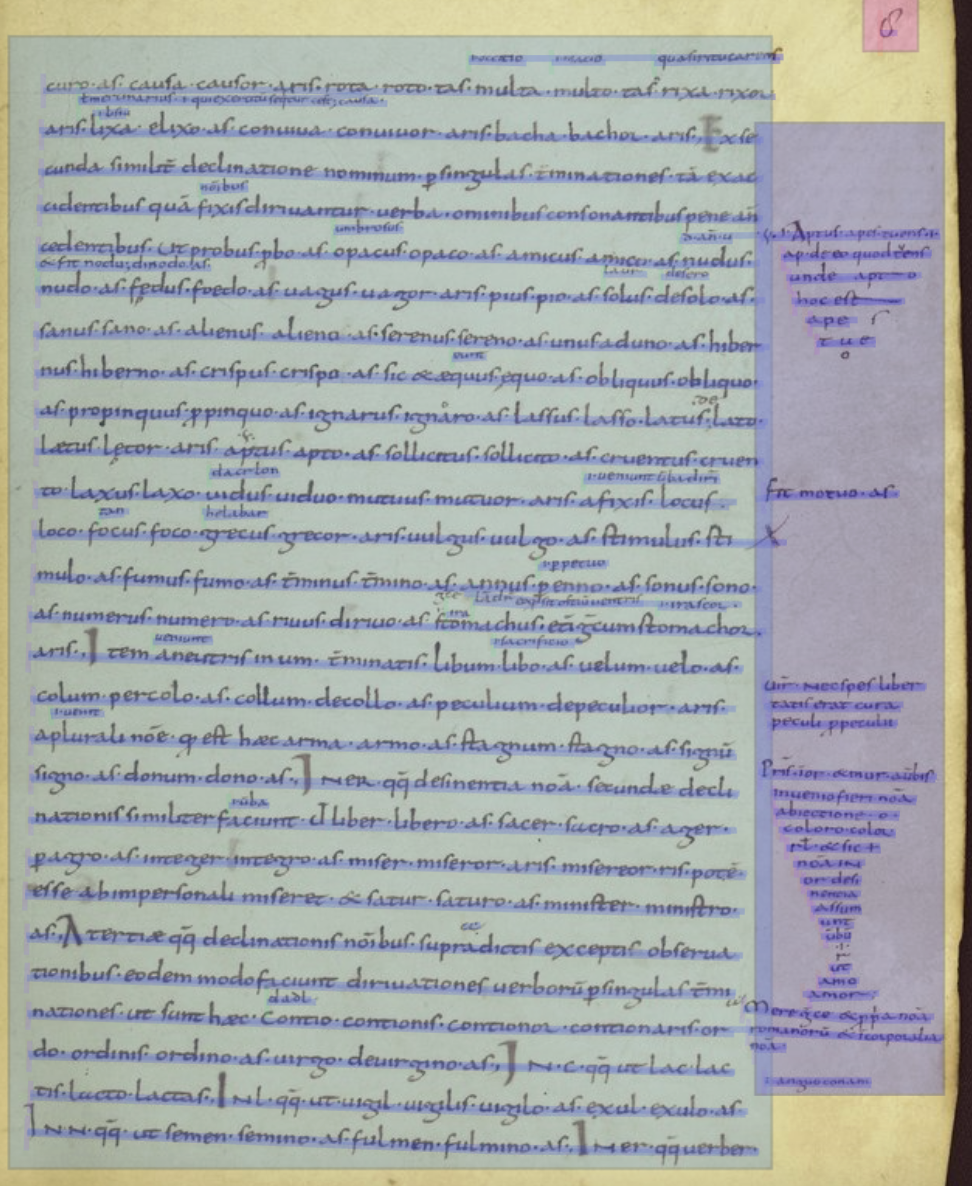
\includegraphics[height=10cm]{YALTAi/test_images/Bodl_Auct.F.4.32.DefaultLine_InterlinearLineYALTAi_f08r.png}
    \caption{folio 6r : Application du modèle YALTAi avec les deux modèles pour les baselines.}
  \end{subfigure}
  \hspace{1cm} % Adjust the horizontal spacing between the third and fourth subfigures
  \begin{subfigure}{0.4\textwidth}
    \centering
    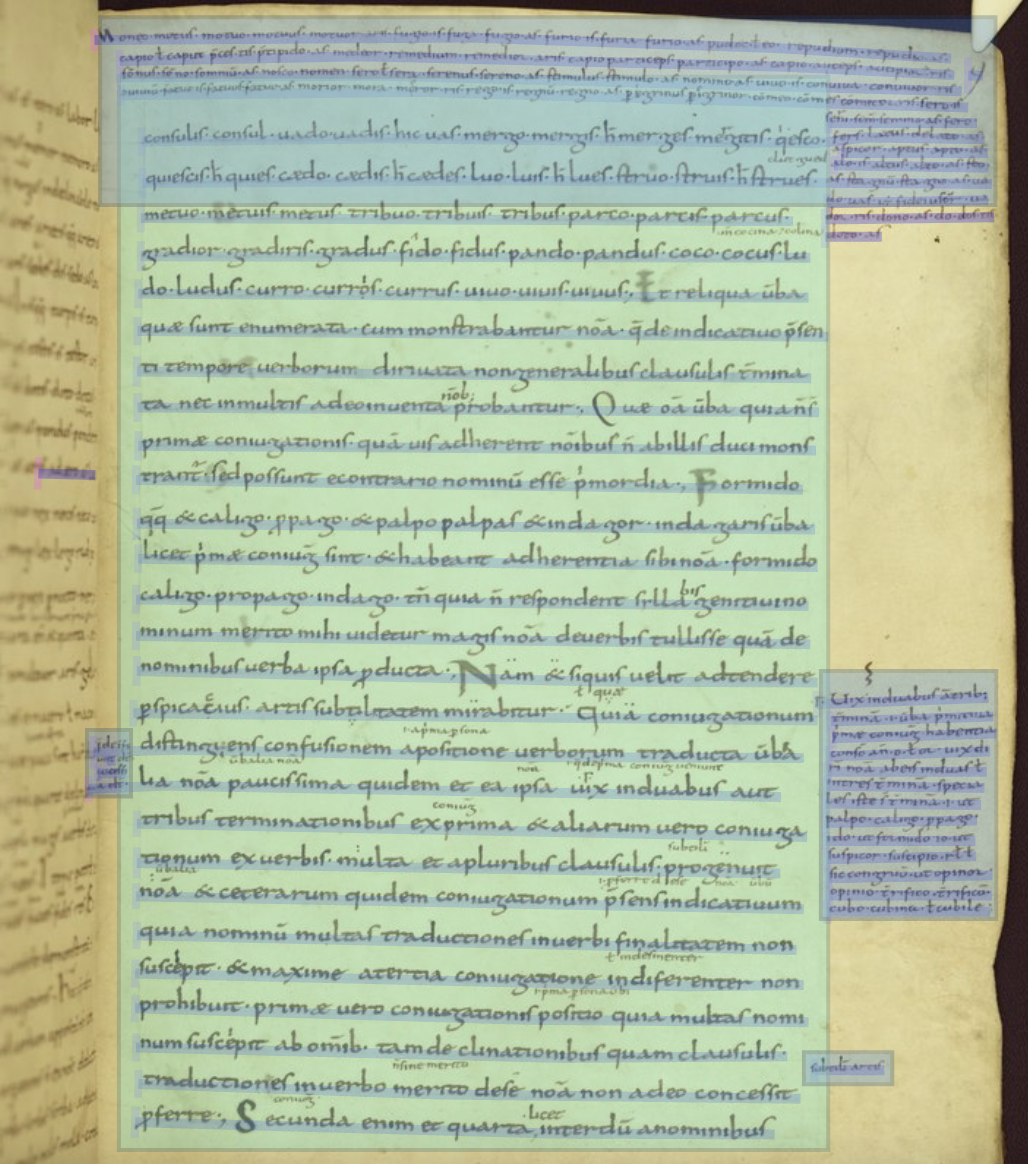
\includegraphics[height=10cm]{YALTAi/test_images/limitations-segmentation-YALTAi.png}
    \caption{Limitations du modèle.}
  \end{subfigure}
  \caption{Résultats qualitatifs sur un corpus de test : Bodl. MS. Auct. F. 4. 32. La boîte englobante est restreinte aux régions rectangulaires et ne peut pas couvrir des polygones complexes tels que ceux en forme de P. Nous notons également que le modèle tente de classifier les lignes du folio précédent lorsque celui-ci est visible.}
  \label{fig:qualitative_YALTAi-kraken}
\end{figure}

\subsubsection{Quality control: HTRVX}
De plus, pour garantir un contrôle qualité lors du stockage de nos informations sur GitHub, nous avons utilisé le logiciel\textit{HTRVX}\footnote{\cite{Clerice_HTRVX_HTR_Validation_2021}}, développé par Thibault Clérice et Ariane Pinche. Ce logiciel est spécifiquement conçu pour vérifier la conformité du schéma XML et l'utilisation de l'ontologie SegmOnto pour la segmentation \footnote{Dans notre cas, nous avons ajouté, dans la liste des ontologies valides, celle de \textit{TironianSignLine}, un type de ligne custom, qui concèrne les lignes contenant des notes tironiennes}. Plus précisément, HTRVX détecte les zones et les lignes non caractérisées, ou mal caractérisées (non conformes au vocabulaire SegmOnto) ainsi que les lignes non associées à une zone. Par conséquent, aucune ligne ne se trouve hors de sa zone dédiée, ni manque une annotation paléographique, assurant la qualité des données. 



\section{Entre segmentation sémantique-éditoriale et visuelle; questions de méthodologie}

Il est important de noter à ce stade les deux approches différentes qui ont été adoptés pour la vérité de terrain fournie pour l'entraînement des modèles de segmentation et de reconnaissance de caractères, par rapport à l'approche adopté pour la partie de transformation des données qui suit. \\


La première approche adoptée est celle de l'exactitude visuelle pour établir la vérité terrain utilisée par les algorithmes de segmentation et de reconnaissance d'écriture. Cette approche ne prévoit pas une division sémantique du contenu, contrairement à ce que nous attendons pour un texte. Ainsi, les annotations marginales sont considérées comme une seule unité, à moins qu'elles ne soient séparées par un espace conséquent. De même, lorsqu'il s'agit de gloses interlinéaires, nous suivons les lignes telles qu'elles sont visuellement représentées, sans forcément respecter une correspondance stricte de 1 ligne = 1 glose. Cette approche simplifie la tâche complexe de segmentation et aide le modèle à généraliser en évitant une segmentation excessive des zones marginales et des lignes interlinéaires. En réalité, la division sémantique des annotations marginales et des gloses interlinéaires est un processus intellectuel qui ne correspond pas toujours à l'apparence visuelle des manuscrits. \\

Cependant, lors de la phase de transformation des données, une approche plus \og{}éditoriale\fg{} a été adoptée afin de faciliter la consolidation sémantique des informations. Dans ce contexte, l'accent est mis sur l'unité de sens plutôt que sur l'aspect visuel \footnote{Distinguer les unités sémantiques des marges n'est pas toujours une tâche facile, en particulier en l'absence de signes de renvoi ou des mots explicites tels que \textit{FINIT} à la fin de chaque annotation marginale, ou de la concaténation du contenu qui correspond à plusieurs lemmes. Cela nécessite une lecture critique et un choix d'attribution des unités de commentaires aux lemmes, qui ne peut échapper à la fluidité du lien entre le lemme et la(les) glose(s) \cite{oSullivan2017lemma}, p.380.}. Toutefois, cette distinction n'est ni nécessaire ni indispensable dans le cas de mises en page moins complexes et non hiérarchiques, où la sortie du modèle pourrait être directement utilisée sans difficulté pour la transformation vers une édition numérique. Malheureusement, les manuscrits glosés présentent une typologie et un contenu complexes, nécessitant une prise en compte attentive de leurs particularités \footnote{Par exemple, l'équipe responsable de la création du dataset DIVA His-DB a choisi de se concentrer uniquement sur la tâche de segmentation en effectuant une segmentation basée sur l'unité visuelle plutôt que sur l'unité sémantique. }. L'unité de sens ne correspond pas toujours à l'unité visuelle, notamment lorsque les gloses s'étendent sur plusieurs lignes ou lorsque les annotations marginales sont fusionnées par manque d'espace, ce qui peut correspondre à des lemmes différents. Pour cette raison, et notamment parce que la connaissance du texte est indispensable, cette étape ne peut pas être automatisée. Ainsi, l'entraînement des modèles de segmentation qui correspondent au mieux à la typologie est une condition \textit{sine qua non}, afin que l'utilisateur puisse se concentrer sur la segmentation sémantique du contenu.\\


\begin{figure}
    \centering
    
    \begin{subfigure}[b]{0.4\textwidth}
        \centering
        \includegraphics[width=3cm,height=10cm]{segmentation_imgs/visual_semantic_segmentation/visual_segmentation.png}
        \caption{Exemple de segmentation visuelle: Lat7499, folio 80r}
        \label{visual_segmentation}
    \end{subfigure}
    % \hfill
    \begin{subfigure}[b]{0.4\textwidth}
        \centering
        \includegraphics[width=3cm,height=10cm]{segmentation_imgs/visual_semantic_segmentation/editorial_segmentation.png}
        \caption{Exemple de segmentation sémantique/éditoriale: Lat7499, folio 80r}
        \label{subfig:sub2}
    \end{subfigure}
    
    % \vspace{1cm}
    
    \begin{subfigure}[b]{0.4\textwidth}
        \centering
        \includegraphics[width=6cm,height=3cm]{segmentation_imgs/visual_semantic_segmentation/visual_segmentation_interlinear.png}
        \caption{Exemple de segmentation visuelle pour les interlignes: Lat7499, folio 79r}
        \label{subfig:sub3}
    \end{subfigure}
    % \hfill
    \begin{subfigure}[b]{0.4\textwidth}
        \centering
        \includegraphics[width=6cm,height=3cm]{segmentation_imgs/visual_semantic_segmentation/editorial_segmentation_interlinear.png}
        \caption{Exemple de segmentation sémantique pour les interlignes: Lat7499, folio 79r}
        \label{subfig:sub4}
    \end{subfigure}
    
    \caption{Différences entre segmentation visuelle/sémantique pour des passages identiques. NB la réduction en une lignes des gloses interlinéaires autonomes.}
    \label{fig:main}
\end{figure}


Pour préserver l'unité sémantique des gloses qui s'étendent sur plusieurs lignes, nous avons adopté une approche éditoriale consistant à transférer la moitié inférieure vers la moitié supérieure de la glose, en utilisant le signe \og{}/\fg{} pour indiquer le saut de ligne tel qu'il apparaît dans le manuscrit. Par exemple, dans la ligne 21 du folio 11r du manuscrit VLO41, la glose \og{}multitudo ho/minum\fg{} sur \og{}uulgus\fg{} est séparée par une barre oblique pour représenter le saut de ligne. Cette approche est également utilisée pour les annotations marginales, qui peuvent être coupées ou commencer au milieu d'une même ligne. Cependant, il est important de souligner que cette approche éditoriale présente certaines limites significatives lorsqu'elle est utilisée pour l'entraînement d'un modèle de segmentation, ce qui justifie la nécessité de la compartimenter en deux étapes distinctes sinon la qualité et la validité de la vérité terrain seraient largement compromises dans ce cas.\\

Cette double approche a été adoptée afin de poursuivre deux objectifs simultanément :
\begin{itemize}
\item Entraîner des modèles plus souples et généraux.
\item Préparer les documents pour une édition documentaire respectant les unités paléographiques de manière sémantique.
\end{itemize}



\subsection{Reconnaissance}


\subsubsection{Modèle de Raiconnaissance pour la Minuscule Caroline}
Jusqu'à très récemment, les anciennes écritures manuscrites telles que la Minuscule Caroline ont été considérées comme imperméables aux outils de transcription automatique comme \textit{kraken}. Certes, il était toujours possible d'entraîner des modèles sur un ensemble de données, mais un modèle générique \og{} clé en main \fg{} capable d'atteindre une précision élevée générale pour plus qu'un manuscrit n'était pas facile à mettre en place \footnote{Sur la complexité que la minuscule caroline pose et les facteurs qui entrent en jeu lors du mélange des modèles différents voir l'article : \cite{hawk2018modelling}}. Depuis 2019 et l'avancement des moteurs OCR qui gèrent les écritures manuscrites, cette difficulté a été partiellement résolue, en permettant une plus grande interoperabilité entre modèles HTR. Depuis le début de l'élaboration de ce mémoire, des modèles généralisés très robustes ont été entraîné par Ariane Pinche, Thibault Clérice et al. pour le projet CREMMA, comme Bicerin et Certado, ou à partir des données en libre accès, comme McManu French pour le français médieval\footnote{ \url{https://zenodo.org/record/6657809\#.ZHYRYuxBx1o}},tous en accès libre \footnote{voir. principalement le travail d'Ariana Pinche \cite{pinche:generic}}. \\


Un tel modèle \og{} clé en main \fg{} nous avait été fourni l'année dernière par Thibault Clérice \footnote{Pour la vérité de terrain de ce modèle voir. \url{https://github.com/rescribe/carolineminuscule-groundtruth}. Le protocole de transcription s'aligne complètement avec nos propres normes de transcription} qui, à en printemps 2022, atteignait le taux de précision  de près de 92\%. Tout de même, une fois appliqué, celui-ci  nécessitait une étape de post-correction pour nos manuscrits, qui comporte de gloses de petite module et dont les polygons des baselines peuvent se superposer.\\

Il est important de noter que l’efficacité de la reconnaissance des caractères et des mots à proprement parler dépend directement du travail réalisé sur la segmentation de la page. En d’autres termes, même si le modèle de reconnaissance des caractères est performant, une segmentation incorrecte ou
incomplète empêchera tout résultat satisfaisant. Pour toutes ces raisons, la plus grande partie de la transcription a été faite manuellement, dans l'optique de \textit{fine-tuner}\footnote{ \og{} Fine tuning ou spécialisation progressive : Il s’agit, dans le domaine de l’intelligence artificielle, d’adapter un modèle préexistant à un jeu de données spécifique à la tâche visée.\fg{} L'ensemble du vocabulaire specialisé HTR et une description minutieuse de la chaîne de traitement se trouve dans le rapport rédigé par Noëmie Lucas, dans le cadre d'une résidence de recherche à la BULAC en 2020-2021 soutenue et publié par le GIS, an libre accès en ligne \url{http://www.bulac.fr/node/2491}
} ou plutôt de personnaliser le modèle fourni pour qu'il réponde à nos besoins . 80\% du jeu de données, a été réservé pour le \textit{fine-tuning} et 20\% pour l'évaluation. La présence de huit mains distinctes au total dans le même jeu de données offre une variété précieuse qui empêche un sur-apprentissage totale sur une des mains et par conséquent permet la réutilisation directe du modèle de reconnaissance. Le modèle final, d'un taux de 98,4\% d'accuracy \footnote{disponible ici: \url{https://github.com/malamatenia/Eutychès/tree/main/data/models}}, a été employé pour la transcription des trois manuscrits qui complètent le dataset, le Lat14097 le BambergMsc30et le Lat7499 de  qui a nécessité une post-correction minimale de notre part\footnote{À l'exception des notes tironiennes, qui ont été déchiffrées par M. Cinato, à qui suis extrêmement reconnaissante pour son aide, sans laquelle leur nature/fonction n'aurait pas été claire.} \\


\textsc{Outils de lecture/ déchiffrement}\\

Afin de vérifier la qualité de notre transcription du texte principal, nous avons comparé notre travail avec l'édition et l'apparat critique de Keil\footnote{\cite{keil1857grammatici}}. Cette comparaison nous a permis de confirmer l'ordre et la coupe correcte des mots\footnote{À ce stade, je tiens à remercier Cécile Conduché pour sa contribution précieuse dans la collation du texte principal du témoin Lat7499, ce qui a grandement facilité la phase de post-correction}. Nous avons ainsi validé certaines de nos intuitions, corrigé nos erreurs et identifié les passages où notre témoin diffère de l'édition de référence, tout en respectant les particularités orthographiques propres à nos témoins.\\

En revanche, la lecture des près de \textbf{4 700} gloses et \textbf{900} annotations marginales, pour la plupart inédites\footnote{Nous avons trouvé quelques fragments de transcription du Lat7499 dans les articles de réference tels que \cite{jeudy1974manuscrits}, \cite{sabbadini1995opere}, et \cite{lemoine1989symptomes} mais rien de substantiel. Si Jeudy Colette avait envisagé une publication des gloses, elle n'a malheureusement pas pu publier une étude incluant la lecture partielle ou complète.}, n'a pas été une tâche facile. Leur forme concise, leur caractère informel, les abréviations employées, ainsi que l'état de conservation de certains manuscrits ont également compliqué notre travail. En cas de doute, nous avons mis en place plusieurs stratégies. Tout d'abord, nous avons effectué une lecture comparative entre nos témoins et d'autres témoins glosés \footnote{En particulier, le BnF.lat.7498 nous a aidés dans la lecture du Bamberg Msc30, de même que le BL MS.Auct.F.4.32 pour le VLO41, étant donné qu'ils partagent une grande partie des gloses}. Cette approche comparative nous a permis de vérifier notre lecture, notamment en ce qui concerne les synonymes ou les annotations marginales. Lorsqu'une comparaison directe n'était pas possible en raison de l'absence de correspondances entre les témoins, nous avons effectué des recherches approfondies dans la Database of Latin Dictionaries (DLD)\footnote{\url{http://clt.brepolis.net.janus.bis-sorbonne.fr/dld/Dictionaries/Search}}, le Thesaurus Linguae Latinae (TLL)\footnote{\url{https://tll.degruyter.com/}} et la Library of Latin Texts de Brepolis\footnote{\url{http://clt.brepolis.net.janus.bis-sorbonne.fr/llta/pages/Search.aspx}}. Ces ressources -accessibles grâce à la Bibliothèque Inter universitaire de la Sorbonne- nous ont permis de comprendre le sens des gloses grâce aux parallèles intertextuels. Cette méthode nous a permis d'obtenir une lecture aussi fiable que possible des gloses, bien que nous ayons parfois rencontré des passages vraiment difficiles ou le déchiffrement était impossible, et des erreurs dans la lecture sont dues à notre relative inexpérience avec le processus de lecture des sources manuscrites\footnote{Dans le cas du VLO41, tous les passages restitués sont soigneusement signalés dans le fichier XML-TEI à l'aide de l'élément <supplied>, qui permet également d'enregistrer le degré de certitude de la lecture proposée. Nous prévoyons d'appliquer la même méthode à nos deux autres témoins.}. \\

En ce qui concerne les normes de transcription, nous avons adopté une approche graphématique plutôt qu'allographétique \footnote{Pour la distinction entre les deux approches \cite{}}. Dans notre cas, étant donné le caractère standardisé de la Minuscule Caroline, cela ne produirait pas de résultats très différents. Le texte a été transcrit aussi fidèlement que possible, avec une intervention minimale de notre part\footnote{Une approche purement graphématique a été utilisée, notamment pour affiner le modèle de base}. Nous avons conservé les caractères diacritiques, les signes spéciaux introduisant les gloses explicatives et les abréviations, car ils sont précieux pour d'éventuelles collations et pour l'établissement du texte. Cependant, une intervention a été nécessaire pour gérer les espaces entre les mots dans les premières pages, qui présentent des caractéristiques de \textit{semi-continua}. Une description détaillée de notre approche et des spécificités de la transcription est disponible dans l'article \cite{clerice2023cremma}. \\

\subsubsection{Quality Control: chocomufin}

Afin de garantir l'application rigoureuse des normes de transcription et la cohérence des données produites, nous avons mis en place plusieurs mesures tout au long du flux de production et de stockage des données. Pour la normalisation des caractères spéciaux issus de \textit{mufi}\footnote{The Medieval Unicode Font Initiative : \url{https://mufi.info/m.php?p=mufi}}, ainsi que pour la vérification de la conformité des fichiers XML ALTO, nous avons utilisé l'outil logiciel \textit{Chocomufin} : CHaracter Ocr COordination for MUFI iN texts\footnote{\cite{Clerice_Choco-Mufin_a_tool_2021}}. Ce logiciel a été développé pour traiter les différentes approches de transcription des données médiévales, en prenant en compte les aspects allographiques et graphématiques, ainsi que les abréviations. L'utilisation de \textit{Chocomufin} nous a permis de valider la compatibilité de notre transcription avec le projet \textsc{CREMMA}\footnote{\cite{pinche2022cremmalab}}, garantissant ainsi l'interopérabilité des données et leur réutilisabilité pour l'entraînement des modèles de reconnaissance automatique. Cette approche globale de contrôle qualité et d'adaptation des transcriptions a assuré la cohérence et la fiabilité des données produites dans le cadre du projet.\\

\subsection{HTR-United}

Pour nous, l'étape finale de l'acquisition des donnés finit avec leur publication en libre accès.\\

En effet, la production de données OCR et HTR peut être à la fois coûteuse et chronophage, nécessitant l'implication d'experts paléographes pour garantir leur validité scientifique. De nombreux projets ne disposent pas toujours des ressources nécessaires pour produire, corriger et maintenir ces données. De plus, l'accès aux données préexistantes revêt une grande importance, étant donné la rapide évolution des algorithmes de reconnaissance et de segmentation. Malheureusement, la production et la publication de nouveaux jeux de données ne suivent pas toujours le même rythme. Dans notre cas, par exemple, les modèles de segmentation et de reconnaissance ont été développés à partir de données mixtes.\\

La recherche et l'accès aux données peuvent également être difficiles en raison du manque de pratiques standardisées pour leur publication et leur accessibilité. De plus, la combinaison de différentes ressources peut être compliquée en raison des variations dans les règles d'annotation et les formats de stockage tels que PAGE, ALTO, et autres. Il est, par conséquent, davantage important de disposer des données en libre accès, avec une description de la stratégie de segmentation et de transcription, afin que plusieurs projets puissent les utiliser pour leurs propres objectifs. C'est là qu'intervient le projet HTR-United, qui offre une solution pour faciliter la production, la recherche et la combinaison de données OCR et HTR. En utilisant cette plate-forme, nous pouvons optimiser l'accessibilité, l'utilisation des ressources existantes et encourager la collaboration au sein de la communauté des sciences humaines. Le partage des données et des connaissances contribue à éviter la duplication des efforts et à accélérer les progrès dans le domaine de la transcription automatique. Nous soutenons pleinement cette initiative et avons donc choisi de stocker nos données dans le Catalogue HTR-United\url{https://htr-united.github.io/tools.html}.


\section{Volet 2:Transformation des données}

\subsection{\textsc{XML-Alto}}

Une fois que le texte a été segmenté, annoté et transcrit, il devient essentiel de choisir le format le plus approprié pour exploiter les données structurées. Parmi les options proposées par eScriptorium, à savoir le format .txt, PAGES et ALTO, le format ALTO s'avère le mieux adapté aux besoins du projet. Il va sans dire que le simple format .txt brut est totalement inapproprié, car il ne respecte ni ne reflète la hiérarchie interne de la mise en page et du contenu. De plus, sa lisibilité est compromise par la confusion des lignes.\\

En revanche, le format XML-ALTO (Analysed Layout and Text Object)\footnote{\url{https://www.loc.gov/standards/alto/}} constitue un standard XML qui permet de représenter la mise en page physique et la structure logique d'un texte transcrit par reconnaissance optique de caractères (OCR). Son utilisation est donc essentielle. De plus, ce format est adapté à la conservation à long terme des données issues de la conversion OCR. Il offre également la possibilité de réutiliser et de transformer les données dans différents formats, ce qui correspond précisément à notre prochaine étape dans le projet.

\subsection{XSL}

Le format final que nous cherchons à atteindre est une édition documentaire en XML-TEI. Pour ce faire, il est essentiel de convertir la sortie de notre transcription, c'est-à-dire les fichiers XML-ALTO, en XML-TEI\footnote{\cite{janes2021towards}}. Dans le but de mettre en valeur l'annotation SegmOnto, nous avons opté pour l'utilisation de feuilles XSL qui regroupent les fichiers ALTO de sortie en y appliquent globalement une transformation. En se basant sur la structure des fichiers ALTO et en appliquant des règles spécifiques vers un format XML-TEI valide, nous pouvons automatiquement obtenir l'ébauche d'un fichier TEI \og{}minimal\fg{}, incluant toutes les informations codicologiques relatives à la pagination, aux lignes principales, aux interlignes, aux notes tironiennes, ainsi qu'aux commentaires en marge annotés avec SegmOnto\footnote{Disponibles également dans notre dépôt Github dans les sous-dossiers XML-XSLT.}. La Figure 2.3 illustre la modélisation de cette transformation de ALTO vers TEI.

\begin{figure}[H]
    \centering
    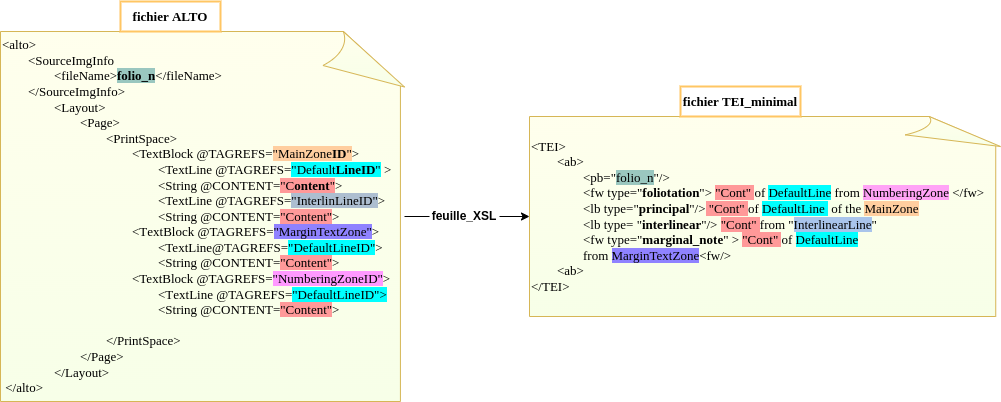
\includegraphics[width=15cm, height=8cm]{pipeline/ALTO_to_TEI.drawio.png}
    \caption{ Transformation des fichiers ALTO à un fichier XML-TEI minimal avec integration de l'ontologie SegmOnto }
\end{figure}


L'interopérabilité et la réutilisabilité des données, ainsi que la possibilité de les transformer en différents formats, sont au cœur des débats en sciences humaines numériques, et cela n'est pas sans raison. Plutôt que d'effectuer un encodage manuel complet, une grande partie de la structuration est réalisée de manière automatique, ce qui permet de gagner du temps tout en garantissant la cohérence des données. Il ne reste plus qu'à compléter/enrichir l'encodage manuellement en définissant les éléments d'intérêt que nous discuterons dans la section suivante. Étant donné les problématiques exposées dans la première partie de ce mémoire, nous avons envisagé notre encodage non seulement comme une pratique d'édition, mais surtout comme une pratique de recherche qui permettra une interrogation et une exploitation des données de manière optimale.

\subsection{XML-TEI}

En examinant la notion d'édition critique et compte tenu de la distance temporelle entre l'original (\textsc{vi}\ieme{} siècle) et les copies qui nous sont parvenus du\textsc{viii}\ieme{} jusqu'à la fin de l'époque carolingienne, ce projet n'a pas pour objectif de remonter à l'original ni de retrouver une variante parfaite\footnote{\cite{cerquiglini1990eloge}}.En effet, la méthod(ologi)e lachmannienne a propagé l'idéologie de la reconstruction de l'\textit{Urtext} archétypal perdu, alors que tout texte connaît différentes réalisations au cours de son histoire.  Cela est particulièrement vrai pour les éditions de gloses et de manuscrits glossés, où l'on considère que:
\blockquote{l’ensemble des interventions faites par les acteurs qui l’ont produit constitue la recension primaire de la collection, quel que soit le nombre de strates qui la compose. [...] Dans le cadre de l’analyse des gloses décrit en termes de relations entre collections et corpus, le système stemmatique de Lachmann ne s’applique pas : il serait vain de vouloir faire remonter une collection de gloses à un modèle identique antérieur, puisqu’il n’a probablement jamais existé\footnote{La même constatation fait Emmanuelle Kuhry, éditrice du \textit{De plantis} glosé \cite{kuhry2020medieval}}. La démarche stemmatique [...] n'a aucun sens dans un contexte de transmission fluide. Il n’y a pas de texte « original » à reconstruire, sinon une source \og{} ultime \fg{}, modifiée et parfois transformée, de proche en proche, au fil des réemplois\footnote{\cite{cinato2015priscien},p.260}}. 
Ce que nous sommes en mesure de détecter, est un noyau cohérent des lemmes/gloses que la totalité de la tradition manuscrite partage. Des méthodes et des outils d'analyse des relations entre collections et corpus de gloses qui offrent une plus grande souplesse se mettent à la disposition des éditeurs comme la phylogénétique et l'analyse des réseaux\footnote{cf. l'édition de \cite{steinova2021glosses}}. Le présent projet vise  simplement à mettre le texte dans son contexte \footnote{Pour une discussion sur les questions numériques que cette recontextualisation implique voir. \cite{pierazzo2011putting}} et à explorer les informations textuelles, paratextuelles et métatextuelles offertes par les témoins. Décontextualiser soit le texte de son paratexte soit l'inverse serait, pour citer Vivien Law \blockquote{rather like the fossil hunter who ignores the strata in which his prize specimen is embedded \footnote{\cite{law1997grammar},p.22}}.\\

Sur les fondements théoriques des éditions critiques numériques, Peter Robinson \footnote{\cite{robinson2001critical}} nomme six aspects essentiels à tenir en compte:

\begin{enumerate}
  \item Une édition numérique critique est ancrée dans une analyse historique des matériaux ;
  \item Une édition numérique critique présente des hypothèses sur la création et l’évolution dans le temps ;
  \item Une édition numérique critique fournit un enregistrement et une classification dans le temps, dans de nombreuses dimensions et avec des détails appropriés ;
  \item Une édition numérique critique peut présenter un texte édité, parmi tous les textes qu'elle propose ;
  \item Une édition numérique critique offre aux lecteurs l’espace et les outils pour qu’ils puissent développer leurs propres hypothèses et modes de lecture ;
  \item Une édition numérique critique doit offrir tout cela de manière à enrichir la lecture.
\end{enumerate}

Tous ces critères peuvent être satisfaits dans un environnement numérique, en tenant compte des spécificités propres au document à encoder. L'absence de contrainte spatiale dans le numérique permet de représenter les données dans leur intégralité, tandis que la flexibilité des outils numériques facilite une interrogation plus efficace de ces données. Cependant, afin de rendre exploitable l'ensemble des informations présentes dans un manuscrit glosé, il est nécessaire de reproduire sa précieuse typologie par le biais de l'encodage. Celui-ci doit offrir les moyens d'analyser toutes les manifestations selon les différents niveaux d'information imposés par une typologie à facettes multiples. Les questions essentielles se rapportent à la structure, à la sélection et à l'encodage des données constituant le corpus. Ce corpus de gloses ouvrira des possibilités d'exploitation aussi variées que le contenu des métadonnées sera organisé de manière à prendre en compte les spécificités inhérentes aux gloses. La qualité des résultats et les possibilités offertes par le corpus dépendront de la richesse et de la diversité des informations encodées, qui serviront à la fois de critères de sériation et d'outils d'analyse. À l'ère du numérique, il ne s'agit plus d'encoder le plus grand nombre d'informations possible, mais plutôt de faire du document une \og{}synthèse structurée des variations observables\fg{}. Le contenu fondamental des collections, à savoir les lemmes et les gloses, doit être encodé de manière à permettre l'application de technologies visant à faciliter l'exploitation, l'exploration et la visualisation scientifiques des données.


\subsubsection{Choix de l'encodage}

Déjà, les avantages d'une approche numérique concernant les manuscrits glosés ont été soulignés par Franck Cinato\footnote{\cite{cinato2015priscien} et \cite{cinato2011perspectives}} et Paolo Monella\footnote{\cite{monella2019digital}}, qui ont travaillé et continuent à le faire sur la modélisation et l'encodage de la tradition manuscrite de Priscien de Césarée, et dont le travail a servi de point d'appui à notre processus d'encodage proprement dit. S'aligner sur les principales pratiques du domaine est crucial pour l'interopérabilité et l'homogénéité des données qui se prêtent à un examen vis-à-vis, comme pour le grand réseau de corpus des \textit{Grammatici Latini}\footnote{Sur ce sujet, la vision et l'entreprise majeure de l'\textit{Index Grammaticus} déjà pendant les années '90 : \cite{lomanto1990index}, les perspectives d'un corpus électronique des GL décrites par Alessandro Garcea dans \cite{garcea2010corpus} et plus récemment, depuis 2020, le Projet ERC PAGES \cite{spangenberg2022pages}}.\\

L'encodage doit fournir les moyens d'analyser l'ensemble des manifestations selon les différents niveaux d'informations dégagés précédemment. Face à ces niveaux, Franck Cinato a adapté des concepts développés dans le cadre plus large de l'organisation des connaissances sur le cas des manuscrits glosés, en suivant le \textit{faceted classification system\footnote{Une classification à facettes utilise des catégories sémantiques, soit générales, soit spécifiques à un sujet, qui se combinent pour créer la base de classification complète. Des facettes subordonnées affinent davantage le sujet.}}. Ces facettes permettent une caractérisation complète de l'entité appelée glose, et consistent en plusieurs dimensions.  L'intérêt d'une typologie complexe lors de la sériation réside dans la \og{}finesse granulométrique\fg{} qui permet des opérations de tri sur de grands ensembles de données. Un encodage qui inclut l'ensemble des informations pivot, comme cela sera mis en évidence lors de la visualisation des données (cf. \textit{infra}), s'avère particulièrement utile pour observer les mouvements de la confection du manuscrit et les préoccupations des glossateurs-compilateurs.\\

\textsc{Mise en page}\\

En considérant que la mise en page joue un rôle fonctionnel plutôt qu'accessoire dans la disposition du contenu intellectuel de l'oeuvre, il est impératif que l'encodage inclue ces spécificités. En effet, la description
\og{} codicologique \fg{} qui s’attache plus à l’aspect formel des gloses, constitue une première facette du système d'analyse. Les deux aspects qui méritent notre attention sont 1) la disposition en colonnes qui rompe le sens de lecture de l'horizontale à la verticale et 2) le type des lignes selon leur environnement et leur fonctionnalité.\\

En ce qui concerne la typologie des lignes, l'encodage, produit de la transformation XSL se présente ainsi : Les \textit{DefaultLines} se sont transformées en 
\begin{minted}{xml} 
<lb type="principal"> 
\end{minted}
et les \textit{InterlinearLines} en :
\begin{minted}{xml} 
<lb type="interlinear">
\end{minted}

Pour le témoin de Bamberg, nous avons également prévu un attribut pour la catégorie des notes tironiennes, que nous encodons de la manière suivante : 

\begin{minted}{xml}
<lb  type="tironian"/>
             <gloss rend="italic" xml:id="p447_l05_o05_a" target="#p447_l05_o05" ana="S22" style="F2">PRAECEP ͭ ͦ ͬ ͥᵇ ͧ ᷤ</gloss>
\end{minted}

Cette information nous servira plus tard lors de l'analyse exploratoire des typologies des gloses.

\subsubsection{Indexation des lemmes}


\begin{flushright}\textit{ «As the starting point for interpreting a text, the lemma is a good place to look for matters relating to the how and the what of reading. It represents a deliberate choice, a dividing up of a text.» }\end{flushright}

\begin{flushright}\textit{ « O'Sullivan(2017), p.373» }\end{flushright}

Une mention préalable importante concerne la nature même des lemmes. Comme déjà évoqué, tout mot ou groupe de mots d'un texte principal peut potentiellement être considéré comme un lemme. Les lemmes, dans un sens ontologique, constituent des segments arbitraires du texte principal qui se comportent en tant qu'entités possédant un degré d'autonomie relatif à leur dépendance du texte. Pour illustrer cela par des exemples concrets, un verbe isolé (tel que \textit{amo}) peut se suffire à lui-même, indépendamment du contexte immédiat ou intellectuel de la phrase. En revanche, un pronom (comme \textit{a quibus}) dépend entièrement de son contexte pour avoir un sens. Ainsi, selon la définition du lemme adoptée, tout segment dont le sens a été augmenté de quelque manière que ce soit constitue un lemme unique.\\

L'indexation consiste à attribuer des références ou des marqueurs spécifiques à des éléments ou des parties d'un texte afin de les identifier et de les retrouver facilement et est une pratique courante dans la recherche des manuscrits glosés. Déjà des chercheurs ont recours à ce système\footnote{Par exemple, Steinovà: \cite{steinova2021glosses} et O'Sullivan: \cite{oSullivanglossae}.} pour leurs analyses. Étant donnée la relative fluidité du texte principal, qui n'est pas entièrement stable en termes d'ordre des mots, ce système d'indexation permet de fixer une position stable pour chaque mot. Cela se révèle particulièrement utile pour le cas d'Eutychès qui a tendance a répéter les exemples, et souvent à gloser les mêmes mots. Ainsi cette pratique permet d'établir un système cohérent pour repérer et comparer les mêmes mots dans différents manuscrits. Parallèlement, cette approche permet de mettre en évidence les lemmes uniques et propres à chaque témoin, ce qui contribue à affiner son profil, comme nous le verrons plus tard.\\

En utilisant les références/identifiants uniques fournies par l'édition critique, nous créons des points de repère communs qui facilitent l'identification des différences entre les versions des lemmes dans chaque manuscrit. Cela permet de mener plus tard des analyses comparatives et de mieux comprendre les variations et les divergences qui peuvent exister, comme par exemple les variantes orthographiques pour une collation critique, qui peut bénéficier l'étude du texte de base, ainsi que des gloses.
Elle permet de mettre en évidence les différences et les similitudes entre les versions d'un texte et de suivre l'évolution et la transmission du texte au fil du temps.\\

Côté pratique, pour encoder un lemme qui est présent dans l'édition de référence de Keil, nous utilisons la structure suivante :

\begin{itemize}
    \item un élément neutre \textbf{seg} qui est plus neutre en sémantisme par rapport à l'élément <lem>\footnote{La définition de l'élément <lem> dans les Guidelines XML-TEI \url{https://tei-c.org/release/doc/tei-p5-doc/fr/html/TC.html\#TCAPLL} précise \og{}N.B. the term lemma is used here in the text-critical sense of ‘the reading accepted as that of the original or of the base text’.\fg{} et est employé pour les variantes textuelles signalées dans l'apparat critique d'une édition après la collation.};
    \item un attribut \textbf{@type} = lemma qui spécifie la valeur sémantique du segment ;
    \item un \textbf{xml:id} unique composé des coordonnées du segment.\\
\end{itemize}

\begin{minted}{xml}
<seg type="lemma" xml:id="p452_l16_o05">Aedifico</seg> :
\end{minted}

Dans cet exemple, l'attribut xml:id unique correspond à la page/ligne/ordre du mot (ou des mots dans le cas des \og{} multi-word units\fg{}\footnote{\cite{oSullivan2017lemma},p. 380}) dans l'édition de Keil. Dans le cas où le lemme n'y figure pas, nous utilisons une logique similaire en attribuant un \textbf{xml:id} correspondant au folio/ligne/ordre du mot dans le manuscrit concerné : \\

\begin{minted}{xml} 
<seg type="lemma" xml:id="f72v_l01_o02">circũstantię </seg> :
\end{minted}

Cela garantit une cohérence dans le système d'encodage pour pouvoir facilement repérer les informations que l'on souhaite.\\

\textsc{Gloses ad-hoc et Gloses marginales}\\

Gloses et notes marginales sont encodées selon une syntaxe différente dans les éditions documentaires, en utilisant la typologie préétablie par la TEI. Ainsi, les gloses sont encodées avec la balise <gloss>, tandis que les annotations marginales sont encodées avec la balise <fw> (forme work), auquel est ajouté un descripteur personnalisé @type= marginal\_note pour préciser leur fonction. Pour les gloses, nous utilisons l'élément préalablement défini par les directives de la TEI, à savoir <gloss>\footnote{Selon le vocabulaire de la TEI : <gloss> (gloss) identifie une phrase ou un mot utilisé pour fournir une glose ou une définition pour un autre mot ou une autre phrase.}, pour encadrer les gloses. Il convient également de noter que chaque glose possède son propre identifiant XML @xml:id, qui est identique à celui du lemme correspondant, suivi d'une extension \textbf{\_a} ou \textbf{\_b} en fonction de l'ordre d'apparition des gloses pour un même lemme (par exemple \textbf{\_a} est souvent réservé pour les gloses et \textbf{\_b} pour les notes marginales).\\

Tout d'abord, il est essentiel d'associer les gloses/annotations marginales aux lemmes correspondants en utilisant les attributs XML @target (pour les gloses) et @corresp (pour les annotations marginales)\footnote{La structure de la TEI limite l'utilisation des attributs à un ensemble restreint à l'intérieur d'un élément, ce qui justifie ces choix contraints.}. Cette démarche permet de reconstituer la structure fondamentale de la relation entre le lemme et la glose, qui constitue l'essence même de notre étude.\\

Une typologie formelle des gloses attestées dans les manuscrits grammaticaux a déjà été formulée par Rijcklof H.F. Hofman\footnote{Hofman, Rijcklof HF. The Sankt Gall Priscian commentary. Part 1. 2. Translation and commentary; Indices. Nodus-Publ., 1996.} à la fin des années 90, typologie qui a été étendue et raffinée par Franck Cinato pour son édition de Priscien glosé. Cette catégorie Sens comprend sept sous-catégories principales (cf. aussi la Figure \ref{irvine_cinato} et l'Annexe à la fin pour la liste complète.) :

\begin{itemize}
\item S1 Prosodique
\item S2 Lexicale
\item S3 Grammaticale (morphologique)
\item S4 Syntaxique
\item S5 Explicative (commentaire)
\item S6 Ecdotiques
\item S7 Notes socio-historiques
\end{itemize}

Ces sous-catégories permettent des subdivisions, ce qui signifie qu'un identifiant unique est attribué à chaque manifestation sémantique de la glose. Par exemple, nous utilisons S22 pour représenter les synonymes et S23 pour les définitions \footnote{Pour la typologie complète, veuillez vous référer à l'Annexe 3 de Cinato (2015)}. Il est certainement plus facile d'attribuer un descripteur typologique à une glose qu'à une annotation marginale qui peut parfois correspondre à plusieurs catégories. Par exemple, il arrive souvent que les notes marginales traitent à la fois du synonyme d'un verbe, de son étymologie ou de sa dérivation nominale. Dans ces cas, nous avons adopté l'approche suivante :
\begin{itemize}
\item Lorsqu'il y a deux typologies, dont l'une est plus courante, nous choisissons la typologie plus rare. Par exemple, entre S22 (synonyme) et S25 (Décomposition d'un mot en ses composantes), nous avons choisi de conserver S25 afin de mettre l'accent sur l'élément novateur.
\item Lorsqu'il y a plus de trois typologies ou lorsque deux typologies sont toutes deux peu courantes, nous avons opté pour le descripteur plus général S5 (Explicative), qui englobe plusieurs fonctions et est plus neutre.
\end{itemize}

De plus, il est possible d'ajouter des descripteurs supplémentaires avec l'attribut @style, pour la taille des gloses/annotations marginales, ce qui est particulièrement important pour effectuer des statistiques sur la taille des gloses/annotations marginales dans nos témoins.\\

\begin{itemize}
\item F1 Signe
\item F2 Morphème
\item F3 Syntagme (nominal/verbal) \footnote{Nous soulignons que la concaténation de plusieurs mots (F2) à la suite pour représenter plusieurs synonymes a été encodée comme F3, dans le but de mettre en évidence la longueur de la glose. Ainsi, un synonyme est représenté par F2, mais si nous avons plus de deux synonymes, nous utilisons F3 pour indiquer qu'il existe une sorte de \og{}et\fg{} ou \og{}uel\fg{} entre les synonymes, formant ainsi un syntagme nominal.}
\item F4 Proposition
\item F5 Paragraphe (> deux propositions)\footnote{Cette typologie est une contribution de notre projet visant à distinguer les annotations-commentaires plus étendues présentes dans les marges.}
\end{itemize}

Il convient de souligner que l'identification des lemmes, l'attribution des gloses/\textit{marginalia} et la caractérisation typologique sont des tâches pré-éditoriales qui nécessitent des choix délibérés en fonction des besoins du projet. Dans notre cas, pour faciliter l'analyse exploratoire et statistique, il est préférable de ne pas trop fragmenter les informations en ajoutant des sous-catégories. Il est important pour le lecteur de garder cela à l'esprit tout au long de cette enquête, et dans toute enquête qui se base sur l'analyse statistique.\\

En pratique, cette modélisation logique se traduit par l'encodage suivant :


\begin{minted}{xml}

 <seg type="lemma" xml:id="p447_l13_o06">indicio </seg> 

<lb type="interlinear"/> <gloss rend="italic" xml:id="p447_l13_o06_a" 
target="#p447_l13_o06" ana="S22" style="F2">agnitione</gloss>
    
\end{minted}


Exceptionnellement, Pour le manuscrit VLO41, il est essentiel, pour établir la diachronie au sein des collections de gloses, de signaler également les changements de scribes\footnote{Un petit guide des critères d'attribution des mains, avec une description détaillée et un échantillon, se trouve dans le document \textit{hand\_attribution\_guide} de notre\href{https://github.com/malamatenia/Eutyches/blob/main/VLO41/hand_attribution_guide.pdf}{dépôt GitHub}}.Il convient tout d'abord de distinguer les mains des copistes et des glossateurs. Par convention, un chiffre est attribué aux copistes (mains 1, 2, 3, etc.) et une lettre aux annotateurs (mains A, B, C, etc.). En fonction du type de collection, les éléments du groupe lexical (lemme et glose) ne viennent pas des mêmes personnes.\\

exemple de cet encodage :

\begin{minted}{xml}

<lb type="principal"/> [...]gur auguro as, in as ut <seg type="lemma" 
xml:id="f11v_l22">nugas</seg> indeclinabile ut [...] 

<lb type="interlinear"/>  <gloss type="S22" xml:id="f11v_l22_a" 
target="#f11v_l22" resp="#B"> uanꝰ  </gloss> 

\end{minted} 

Pour les annotations marginales, nous utilisons une syntaxe similaire: \\

\begin{minted}{xml} 


<lb type="principal"/>INCIPIT ARS <seg type="lemma" 

xml:id="p447_l01_o00">EVTICII </seg>  DE VERBO :
             
<fw 
    type="marginal_note" xml:id="p447_l01_o00_a" corresp="#p447_l01_o00"
    ana="S54" style="F5"
             
    <lb type="principal"/>Eutex, euticis. Inde euticius, euticii Et 
    Reꝗrendũ in calce istius libelli cur euticius uocatur 
</fw>
\end{minted}


\textsc{Gestion des colonnes}\\

Un encodage spécifique aux colonnes est utilisé pour préserver l'ordre des lignes et des couples lemme-glose, ce qui revêt une importance potentielle pour la transmission du texte. L'exemple suivant est un extrait d'encodage représentant deux colonnes successives du folio 4r du VLO41 (le seul témoin dans notre jeu de données à présenter cette mise en page particulière), dont certaines lignes principales sont glosées. De nouveau on se sert de l'élément <fw>, cette fois de \@type \og{}colonnes\fg{} pour encadrer les groupes de colonnes. Au sein de cette structure, des éléments vides <cb> numérotés, indiquent l'ordre d'apparition dans la page. \\

\begin{minted}{xml} 
<fw type="colonnes" n="f04r">
    <cb n="1"/>
                              
        <lb n="01" type="principal"/> ut 
        <seg type="lemma" xml:id="f04r_c1_l01" >nuntius</seg>
                              
        <lb type="interlinear"/>
        <gloss   type="S22" xml:id="f04r_c1_l01_a" 
        target="#f04r_c1_l01" 
        resp="#B"> legatꝰ </gloss> 
                              
        <lb n="02" type="principal"/> nuntio. nutias. 
               
        <lb n="03" type="principal"/> 
        <seg type="lemma" xml:id="f04r_c1_l03">Sotius</seg>
                              
        <lb type="interlinear"/>
        <gloss type="S22" xml:id="f04r_c1_l03_a" 
        target="#f04r_c1_l03" resp="#B">comes uicinꝰ </gloss>
                              
        <lb n="04" type="principal"/> Sotio. sotias 
                              
        <lb n="05" type="principal"/>
        <seg type="lemma" xml:id="f04r_c1_l05">Sautius</seg>
                              
        <lb type="interlinear"/>
        <gloss   type="S22" xml:id="f04r_c1_l05_a" target="#f04r_c1_l05"
        resp="#Α"> uulneratus </gloss>
                              
              [...]
              
    <cb n="2"/>
        
        <lb n="01" type="principal"/> Radio. radias.
                                    
        <lb n="02" type="principal"/> consilium 
                                    
        <lb n="03"  type="principal"/> consilior c̃siliaris
                                    
        <lb n="04" type="principal"/>
        <seg type="lemma" xml:id="f04r_c2_l04">conciliũ </seg>
                              
        <lb type="interlinear"/>
            
        <gloss type="S22" xml:id="f04r_c2_l04_a" target="#f04r_c2_l04"
        resp="#B">iudiciũ </gloss> 
            
             [...]
            
</fw>

\end{minted}

\textsc{Citations et \textit{Graeca}}\\

Au couple indissociable lemme-glose et à la mise en page s'ajoutent deux aspects fondamentaux du \textit{De uerbo} et de sa tradition textuelle : les \textit{graeca} (mots ou expressions en grec) et les citations. Ces deux éléments revêtent une importance philologique et culturelle particulière dans l'histoire des textes linguistiques, comme cela a déjà été mentionné.\\ 

Comme mentionné précédemment, le \textit{De uerbo} a été composé à Constantinople, dans un environnement linguistique principalement grec destiné à un disciple hellénophone. Cela explique pourquoi Eutychès, bien que moins fréquemment que son maître Priscien, compare les conjugaisons des verbes latins et grecs, et semble parfois traduire en grec afin d'expliquer le latin, en particulier dans le deuxième livre. La présence d'équivalents grecs dans l'ouvrage répondait aux besoins du bilinguisme grec-latin qui caractérisait Constantinople au \textsc{vi}\ieme{} siècle. Cependant, cela a posé un énorme problème aux scribes de l'Europe latine médiévale, qui ont progressivement perdu leurs connaissances en grec. En conséquence, les mentions de \textit{Graeca}, lorsque présentes, comportent souvent des erreurs significatives, ce qui les rend précieuses pour la \textit{recensio} (la critique du texte). Dans l'exemple suivant tiré du folio 23v, Eutychès ressent le besoin de se référer au terme grec pour \og{}fond\fg{}, à savoir $\Pi \Upsilon \Theta \ M \ H \ N $, que le copiste a retranscrit avec l'orthographe phonétique, précieux indice pour la prononciation des termes grecs. \\ 

\begin{minted}{xml}

[...] a nomine qđ est fundus id est 
<foreign xml:lang="grc"> ΒΥΘΕΜΕΝ.</foreign>

\end{minted} 

D'autre part, les citations provenant d'œuvres littéraires revêtent également une grande importance pour la \textit{recensio}. Elles fournissent une référence stable permettant d'évaluer la qualité de la  \og{} Latinité \fg{} du copiste ou de l'exemplaire utilisé. Il convient de souligner l'importance des citations des auteurs classiques dans la transmission des savoirs pendant le Haut Moyen Âge. En effet, parmi toute la littérature profane, ce sont principalement les manuscrits contenant les \textit{Artes} ou des traités à visée pédagogique de l'Antiquité tardive qui ont été constamment recopiés à travers les siècles. Ces manuscrits revêtent une grande importance en tant que sources précieuses pour la transmission des textes. Même si on avait cessé de recopier Cicerón, Virgile, Horace, en continuant à recopier Donat, Charisius, Phocas, Priscien et les autres grammairiens de l'Antiquité tardive, que l'on a pu un jour reprendre goût à, lire et à recopier Virgile, Cicerón, Horace. Cette circonstance seule suffirait à démontrer que les manuscrits grammaticaux ne sont pas simplement des recueils parmi tant d'autres \footnote{\cite{holtz1978typologie}, p.252}. Luca Martorelli a dressé une liste détaillée des 141 citations présentes chez Eutychès, en enrichissant les références de Lindemann \footnote{\cite{lindemann1833corpus}}, accompagnée de notes critiques sur les passages où Eutychès s'écarte de l'original.\footnote{\cite{martorelli2017citazioni}}. C'est à l'aide de cette liste que nous avons pu localiser avec précision les nombreuses citations et leur associer un lien vers l'édition critique la plus récente, à condition que ça soit en ligne\footnote{notamment vers le {\href{http://www.perseus.tufts.edu/hopper/}{Perseus Digital Library}},ou bien sur {\href{https://archive.org/}{archive.org}}.}. Exemple d'encodage : \\

\begin{minted}{xml}
    <lb type="principal" break="no"/> VIII 
        <quote type="poetry"> has forte inuisitis aras
            <ref target="http://www.perseus.tufts.edu/hopper/text?doc=
            Perseus\%3Atext\%3A2008.01.0498\%3Abook\%3D1" resp="#LM"> 
            Stat. Theb. 1, 668</ref>
        </quote>
\end{minted}


Dans un environnement <quote>, on indique le genre auquel appartient la citation, prose ou poésie, ainsi que le responsable (@resp\footnote{Dans la plupart des cas, il s'agit de Luca Martorelli, sauf lorsque nous avons dû faire référence à une édition différente, disponible en ligne (et changer par la suite les coordonnées de référence). Dans ce cas la @resp est nous.}) des coordonnées de la référence (à l'intérieur d'un <ref>) et le lien (à l'aide de @target) vers le passage original. \\

Faute de temps, l'annotation des \textit{Graeca} et des citations n'a été effectuée que pour le manuscrit VLO41, qui a été traité en premier lors de la première année du Master. Cependant, il convient de noter que tous les manuscrits présentent des orthographes intéressantes des termes grecs, en particulier le manuscrit Lat7499, qui semble se rapprocher le plus de l'orthographe canonique. Dans une étape ultérieure de notre recherche, il serait intéressant d'élargir cette annotation à tous les manuscrits et de mener une étude comparative des termes et des citations afin de pouvoir regrouper les manuscrits en familles. Cela permettrait d'obtenir des informations précieuses sur les relations entre les différents témoins du \textit{De uerbo}.\\


\subsubsection{Questions de normalisation/lemmatisation}

Bien que la TEI offre la possibilité de normaliser le texte tout en conservant les leçons originales, nous avons décidé de ne pas procéder à une normalisation. Ceci est dû à la nature particulière du contenu grammatical et à la façon dont nous souhaitons traiter ces textes. Il est important de noter que tous les outils numériques ne conviennent pas nécessairement à tous les types de données. Cette question n'est pas nouvelle et a été abordée dès les années 90 par Valeria Lomanto et Nino Marinone lors de la conception de l' \textit{Index Grammaticus}\footnote{\cite{lomanto1990concordance}}. Ils se sont interrogés sur la meilleure pratique à adopter pour étudier les co-occurrences des termes dans le corpus des \textit{GL}. En envisageant la création d'un \textit{Lexicon} (un thésaurus composé des entrées d'un dictionnaire), ils ont souligné que : \blockquote{[...] it is not very \textit{suitable} for grammarians in that it involves \textit{lemmatization} and, as it provides \textit{no context}, it cannot reveal one of the salient characteristics of the\textit{Artes}, namely its use of a sort of formulaic language present with \textit{slight variations} in every work. [...] The decision not to lemmatize derives both from the particular nature of the texts and from the future users of the concordance. In the \textit{artes} a high percentage of forms is represented by \textit{isolated graphemes} or by isolated morphemes or, in the chapters on metre, by units which are not linguistic but rhythmic (e.g. armaui rumqueca etc.). Moreover, lemmatization, while it requires a reliable critical text, necessarily
directs, if it does not condition, the interpretation.}

Une intervention éditoriale qui implique une correction en masse des \og{}erreurs\fg{} commises par les copistes, comme c'est le cas dans l'approche de Keil, va à l'encontre d'une étude minutieuse des variantes grammaticales utilisées par les copistes, qui fournissent de précieuses informations sur leur propre niveau de maîtrise du latin. Pour reprendre les mots de Vivien Law\footnote{\cite{law1982insular}, p. 107} :

\blockquote{It is of the utmost importance for future research that editors be scrupulous in their treatment of the texts before them. All departures from the text offered by the manuscripts should be signaled. Emendations, particularly in passages borrowed from Classical grammarians, should be undertaken sparingly and indicated as such in the text. Editorial policy, with regard to orthography, should be stated at the outset: the reader should be aware of how far the text before him differs from what a medieval student might have read. There is no justification when editing a medieval grammatical text for wholesale ‘normalisation’ to Classical conventions; such a practice will cause havoc in alphabetical lists and reflect a misleading image of the author’s Latinity.} 

La normalisation consiste à uniformiser la casse des noms communs, à harmoniser les différentes orthographes pour un même terme sémantique, les dates et les chiffres, ainsi qu'à développer les abréviations afin de procéder à une lemmatisation. La lemmatisation associe à ces formes normalisées un lemme correspondant à l'entrée d'un dictionnaire et une catégorie grammaticale. Par conséquent, elle met en avant le niveau sémantique, car sa principale fonction est de définir les différents sens de chaque terme, d'établir des relations de sens et de tracer la frontière poreuse entre polysémie et homonymie. Ainsi, elle représente l'aboutissement d'une tradition philologique et exégétique si solidement ancrée, à l'issue d'une édition, qu'elle permet au savant d'aborder les problèmes de sens les plus délicats.\\

Pour toutes ces raisons, nous avons opté pour une édition documentaire qui reflète au mieux l'état de la langue tel qu'il est présenté dans le manuscrit, ainsi que le choix des abréviations. Les éditions diplomatiques des grammaires peuvent constituer une ressource particulièrement précieuse pour les historiens de l'éducation et de la linguistique, car les enseignants et les penseurs médiévaux ne disposaient pas d'éditions critiques idéalisées dans leurs bibliothèques. Ils devaient se contenter des copies réelles à leur disposition, avec toutes les erreurs, les malentendus et les omissions qu'elles pouvaient comporter.\\

Une granularité aussi fine, adaptée à nos données, permet l'exploitation précise du texte à deux niveaux. Tout d'abord, il est essentiel de préserver les informations de mise en page afin de conserver leur valeur et leur signification. Ensuite, il est primordial d'interroger le texte de manière approfondie en extrayant les balises d'intérêt pour une comparaison interne ou entre les différents témoins, ce que nous aborderons dans la troisième partie de ce mémoire.\\

\subsubsection{Aller plus loin}

Étant donné que plusieurs témoins ont déjà été transcrits, il est important de développer une stratégie globale d'encodage pour un éventuel plan d'édition. Cela inclut tous les modules, éléments et types d'attributs, et nécessite une application rigoureuse du modèle abstrait d'encodage. Cette approche constitue la clé d'une analyse comparative cohérente de l'ensemble des données fournies par les éditions documentaires individuelles. Afin de garantir la cohérence de notre encodage, il est recommandé d'utiliser des règles Schematron. Ces règles, en complément de la documentation ODD, permettent de valider la structure d'un document XML en définissant des contraintes complexes. Cette approche est particulièrement bénéfique pour un encodage précis, tel que celui que nous proposons. En adoptant cette méthodologie, nous pouvons nous assurer que l'ensemble de nos données et métadonnées sont valides, cohérentes et prêtes à être exportées et utilisées pour des requêtes complexes.\\

\begin{figure}[H]
    \centering
    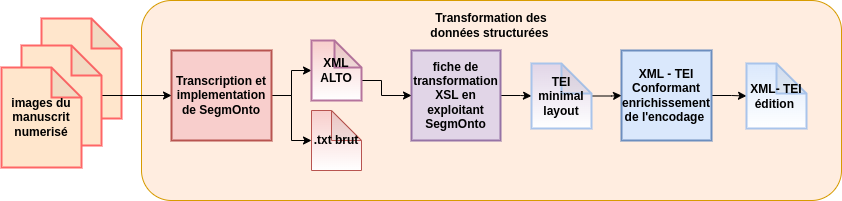
\includegraphics[width=18cm, height=4cm]{pipeline/horizontal_pipeline_texte.png}
    \caption{ Rappel du pipeline  : Modélisation des opérations de transformation des données brutes en données structurées jusqu'à l'encodage complet (axe horizontale)}
\end{figure}

En même temps, il sied de se pencher sur quelques considérations techniques. Sans aucun doute, l'identification, la vérification et le balisage des paires lemmes-gloses ont été les tâches les plus laborieuses et complexes de l'encodage. En raison des multiples attributs spécifiques et des identifiants XML requis pour chaque élément, le processus visant à atteindre le niveau de granularité souhaité s'est révélé à la fois chronophage et fastidieux. Comme l'a déjà constaté Franck Cinato\footnote{\cite{cinato2015priscien}, p. 211}, un encodage aussi détaillé présente un double aspect contraignant : \blockquote{Une telle approche se heurte à la limite imposée par la durée que réclame l’étape de marquage des types selon des codes informatiquement exploitables. Toutefois, la lourdeur du système se trouve compensée par l'utilité de l'interrogation.} Malheureusement, étant donnée la nature critique de ce balisage, cette étape ne peut pas être entièrement automatisée. Toutefois, de nouvelles approches HTR (Handwritten Text Recognition) proposent des modèles mixtes de reconnaissance et d'extraction des \og{}entités nommées\fg{} à partir d'un corpus d'entraînement\footnote{cf. par exemple \url{https://teklia.com/blog/202212-nouveaux-modeles/}}, ce qui semble prometteur pour l'avenir de l'indexation automatique des lemmes et des gloses dans un corpus délimité. \\


\section{Modélisation}

Avant de procéder à l'analyse exploratoire des données, il est important d'élaborer un modèle conceptuel qui permettrait de mieux décrire nos données et de soulever les bonnes questions en fonction des problématiques actuelles de l'état de l'art. Ce processus de modélisation adéquate du discours théorique sur l'érudition marginale, ainsi que des méthodes, outils et données en tant que système nécessitant une clarification, est essentiel pour pouvoir ensuite effectuer des observations ciblées sur nos données.\footnote{Ce chapitre constitue une version retravaillée d'un devoir de validation pour le cours \og{} Humanités numériques et computationnelles appliquées à  l’étude de l’écrit ancien\fg{} de notre directeur de mémoire M Peter Stokes à l'EPHE.}
Pour justifier notre approche de modélisation et pour assurer que le modèle soit applicable, pertinent et utile, il est essentiel de prendre certains éléments en considération : 

\begin{enumerate}
\item Du point de vue du contenu, il est important de prendre en compte la nature des données dont nous disposons à la fin de la chaîne numérique mise en œuvre, ainsi que la nature des éléments qui portent un sens;
\item Du point de vue méthodologique, il est nécessaire de créer un modèle qui soit à la fois suffisamment représentatif du contenu et qui ne révèle que la structure de base, sans ajouts superflus;
\item Du point de vue technique, il est essentiel de considérer le type d'implémentation numérique envisagé.
\end{enumerate}


Ceci dit, notre approche reconnaît avant tout l'importance de la matérialité des nos témoins manuscrits glosés. Ainsi, les caractéristiques codicologiques et paléographiques occupent une position centrale, suivies de leur interprétation sémantique. Il est crucial de ne pas inverser cet ordre, car cela risquerait d'imposer des interprétations préconçues sur le matériel. Notre objectif ultime est en effet d'appliquer le modèle afin de mieux comprendre le matériel lui-même, plutôt que de prendre a priori des décisions sur la relation entre les témoins.\\

Cette réflexion aboutit à la proposition d'un modèle comportant trois groupes d'entités distincts : 1) les métadonnées (section blanche), 2) les éléments codicologiques et paléographiques (section verte et rose), et 3) le contenu sémantique minimal (section orange dans la Figure \ref{fig:modeleconceptuel}. En ce qui concerne les métadonnées, il s'agit des informations externes qui fournissent des détails sur nos données et qui sont nécessaires pour caractériser les conditions et les mécanismes de la tradition manuscrite médiévale, comme discuté en cours. Par conséquent, nous consacrerons la suite de notre exposé à la discussion des entités clés de notre modèle, qui constitue une adaptation du modèle conceptuel conçu lors du séminaire de M Stokes \og{} Humanités numériques et computationnelles appliquées à  l’étude de l’écrit ancien\fg{}.

\subsection{Le modèle conceptuel}

\begin{figure}[H]
    \centering
    \includegraphics[height=10cm, width=18cm]{modelisation_graphs/model_conceptuel.png}
    \caption{Le modèle conceptuel du \textit{de uerbo} augmenté. Adaptation du modèle conçu en cours pour nos besoins.}
    \label{fig:modeleconceptuel}
\end{figure}

\subsubsection{Précisions sur des notions d'oeuvre, d'auteur et de texte}

Avant toute chose, il est impératif de définir les éléments centraux de notre structure.\\

Après avoir pris en compte la nature fluide des œuvres glosées et des commentaires marginaux, nous avons accordé une réflexion approfondie à la compréhension de l'entité \og{}Œuvre\fg{} dans nos données. Il est important de se demander quelle est l'œuvre intellectuelle que nous modélisons. Une première distinction de contenu peut être faite à l'intérieur de la page du manuscrit : le texte principal et les différentes couches d'annotation. Au lieu de séparer ces deux niveaux hiérarchiques (texte principal vs. annotations) et de créer deux entités distinctes pour définir l'œuvre, nous avons opté pour une définition plus neutre qui découle \og{}naturellement\fg{} des données elles-mêmes. Étant donné que nous avons exclu de notre étude les témoins où le texte apparaît sans ajouts peritextuels, nous nous intéressons nécessairement et uniquement à l'ensemble de la tradition qui présente différents degrés d'annotations. Ainsi, par \og{}œuvre augmentée\fg{}, nous entendons ici une entité non-matérielle/conceptuelle qui englobe toute annotation explicative postérieure au texte principal, sans faire \textit{a priori} de distinction sémantique entre \og{}glose anonyme\fg{} et \og{}commentaire éponyme\fg{}. Notre objectif est de mettre l'ensemble du contenu au même niveau, sans imposer a priori une hiérarchie de genre entre nos témoins, et de laisser, dans la mesure du possible, les données s'exprimer sur leur structure, dans une tentative de rendre nos observations objectives.\\


La notion d'  \og{}Auteur\fg{}, elle aussi demeure ambiguë, compte tenu de l'acceptation d'une \og{}oeuvre augmentée\fg{} qui englobe un matériau polyvalent, fluide et anonyme. La remarque de Holtz\footnote{\cite{holtz1978typologie}, p.258} sur la question d'autorité de la glose interlinéaire est d'importance fondamentale : \og{} Ce système de glose n'arrive que très imparfaitement à constituer un véritable commentaire. En effet, il faut que d'une glose à l'autre apparaisse une certaine unification, afin que l'on sente la présence d'un auteur, la continuité d'une méthode de lecture et d'interprétation\footnote{Pour l'importance d'autorité textuelle au Moyen-Âge voir l'article de Minnis : \cite{minnis1988significance}}.\fg{}. Dans notre cas d'étude, l'auteur peut tout aussi bien être anonyme, puisque la plus grande partie de la contribution marginale demeure anonyme. Cependant, il peut également être \og{}éponyme\fg{}, c'est-à-dire identifié rétrospectivement à un maître ou à son atelier, en se basant sur la détection d'un style témoignant d'une véritable culture scolaire, telle que celle de Rémi d'Auxerre\footnote{Le commentaire \textit{in catena} transmis dans les témoins du \textit{de uerbo} reste anonyme sur le plan factuel, et ce n'est qu'en comparant ou en associant les éléments que Rémi d'Auxerre peut être identifié. Pour plus d'informations sur les caractéristiques de l'atelier auxerrois, voir la discussion de Holtz et Lobrichon dans \cite{iogna1991ecole}, ainsi que celle de Lutz sur l'\textit{accessus} identifiable de Rémi d'Auxerre dans \cite{lutz1960one}.}.Nous notons que les commentaires sont des entités complexes et que leur relation au texte principal ainsi que leur degré de dépendance sont beaucoup moins clairs. À cet égard, nous citons Kraus: \og{For commentaries are readings: no matter what the auctoritas of a commentator (and it can be considerable), a commentary is first and foremost an interpretation. Neither the meaning of a text nor the problems perceived as obstructing/complicating that meaning are there to be found; both are created by the readers. Owing on the one hand (perhaps) to its ancient pedigree, and on the other (probably) to its dependence on another text, it is a particularly orphaned interpretation, in which the status of the commentator-as-author has been progressively blurred, till the “I” of the commentator tends toward the mute\footnote{\cite{kraus2002introduction}, p.5.}.\fg{} \\


Nous soulignons également que l'entité \og{}Texte\fg{} se trouve barrée dans notre modèle. Le texte d'Eutychès, bien qu'étant présent sur la page, ne sert qu'en tant que point de départ pour notre étude. Les annotations, tant sur le plan matériel qu'intellectuel, ne dépendent pas du texte en tant qu'entité prédéfinie, mais du lemme. Progressivement, le centre d'intérêt ne réside plus dans le texte ancien lui-même, mais dans sa réception/interprétation et la manière dont celle-ci prend forme en dehors du texte. Cette distance par rapport à la source marque simultanément une proximité avec le lemme. Cette observation implique une conception de la transmission des gloses qui accorde une attention primordiale au lemme, agissant en tant que référence d'un lieu à expliquer\footnote{\cite{oSullivanglossae}, p.136}. Ainsi, chaque mot du texte constitue un topos interprétatif indépendant, offrant d'innombrables possibilités d'annotation, que ce soit en lien avec son contexte ou de manière indépendante. C'est le couple indissociable lemme-glose/annotation qui prévaut sur le concept plus vague et générique de \og{}texte-paratexte\fg{}. C'est pourquoi une distinction importante est introduite dans notre modèle, et l'entité \og{}lemme\fg{} est ajoutée, substituant le texte. \footnote{\cite{cinato2015priscien}, p.187}.


\subsubsection{Entités Codicologiques et Paléographiques}

Après avoir effectué ces distinctions et clarifications importantes, nous abordons le cœur même de la modélisation, à savoir les différents états des annotations présentes sur la page et leur relation avec l'aspect paléographique. Deux axes principaux caractérisent naturellement une annotation par rapport au texte : sa disposition et les éléments d'écriture.\\

Même si cette partie n'est pas exploitée directement dans notre étude, il convient de noter que les différents styles d'écriture constituent une langue secondaire qui encode un texte ayant une signification sociale au-delà de ses valeurs graphémiques et lexicales, à savoir du point de vue codicologique. Les styles d'écriture servent avant tout de marqueurs d'autorité institutionnelle. À l'époque carolingienne, le lemme et le commentaire qui l'accompagne ne se distinguent pas graphiquement par leur \og{}type\fg{}, mais ce sont principalement la différence de module et d'exécution qui marquent leur hiérarchie\footnote{Plus tard, au bas Moyen-Âge,  on observe un retour de l'opposition formelle entre les deux niveaux, par exemple avec l'alternance entre l'écriture gothique et la \textit{notula}.}. C'est pourquoi la disposition occupe une place encore plus importante dans la hiérarchisation des deux niveaux de lecture. Le texte principal, placé au centre et rédigé dans un module normal, s'affirme en tant qu'autorité, tandis que le \og{}paratexte\fg{}, situé en marge ou en interligne et écrit en plus petit module, dépend du texte principal. Cette distinction n'est pas seulement visuelle, elle revêt également une dimension intellectuelle, car elle met l'accent sur la lecture du texte principal en tant que point central d'intérêt. Les caractéristiques codicologiques et paléographiques véhiculent plus qu'une simple signification structurelle; elles confèrent une notion d'autorité. Entre les couches éparses de gloses anonymes, dans les témoins plus anciens, et le texte d'Eutychès, le centre d'intérêt demeure, dans cette configuration, le sens du texte principal.\\

Quant au commentaire marginal, ce constat s'affirme avec une force particulière : en effet, la partie du commentaire à insérer était bien plus volumineuse que le texte commenté lui-même. Malgré leur module réduit, les annotations marginales et interlinéaires parviennent à imposer, grâce à leur volume, leur autorité par rapport au texte principal\footnote{\cite{zetzel2005marginal}}. En cherchant à donner la parole aux données, nous nous alignons sur l'idée selon laquelle un message culturel inhérent est encodé à la fois dans la glose et dans le format du texte lui-même. L'attente du commentaire et de la glose faisait donc partie intégrante de l'expérience de réception et d'interprétation, constituant un processus de négociations continues entre l'autorité du texte et une deuxième autorité plus récente, représentée par la glose. C'est de cette dynamique que naît un dialogue permanent, momentanément figé dans une forme conventionnelle sur la page du manuscrit\footnote{\cite{irvine1994making}, p.390}. Ainsi, dans notre modèle, le \og{}Module\fg{} de l'écriture (et non le \og{}Type\fg{}) est directement lié à la \og{}Disposition\fg{} du texte.\\ 

Toutes ces informations sont prises en compte avant même la lecture et la construction du sens verbal du texte. Une glose est comparable à un photon, elle participe à la fois à deux réalités distinctes : une réalité matérielle et une réalité sémantique. Elle constitue à la fois un élément du processus herméneutique et une manifestation physique d'une pratique d'annotation\footnote{\cite{blom2023glossing}}. Ainsi, les deux approches, celle de la \og{}structure du document\fg{} et celle de \og{}l'expression textuelle\fg{}, se rapprochent et se chevauchent partiellement. Cette constatation met en évidence l'importance d'une double approche sémantique et structurelle lorsqu'il s'agit d'étudier les gloses. Il est essentiel de prendre en compte à la fois le sens et la structure des annotations pour une compréhension complète de leur rôle et de leur signification.

\subsubsection{Attributs sémantiques}

Un aspect très important à prendre en compte dans notre modélisation concerne la relation entre la matérialité et la sémantique du manuscrit grammatical glosé (partie orange du modèle). Après avoir examiné les aspects formels des annotations, il est temps d'explorer leurs implications sémantiques. Les concepts qui sont visibles à l'œil d'un expert lors d'une lecture rapprochée (comme la distinction entre glose et commentaire marginal) ne sont pas nécessairement compris en tant que tels par un modèle statistique. C'est pourquoi des informations formelles telles que le \og{}type\fg{} de glose interlinéaire ou marginale et leur \og{}forme\fg{}, c'est-à-dire la taille de la déclaration, peuvent aider à modéliser le matériel de la manière la plus abstraite et fidèle possible aux manuscrits, en évitant d'ajouter des informations et interprétations supplémentaires. Cependant, il est important de noter que ce processus dépend largement de notre interprétation du contenu explicatif, et cette partie est la seule qui ne découle pas directement des données, mais constitue une classification que nous appliquons. Nous avons déjà mentionné dans notre chaîne de traitement comment nous utilisons cette typologie et les biais potentiels que cela peut entraîner (voir Figure 2.1 dans le chapitre XML-TEI).\\

Plus précisément, en ce qui concerne l'encodage de la taille des annotations, il est important de noter qu'il existe une correspondance entre l'emplacement des gloses dans la page (interlinéaires ou marginales) et la longueur de leur contenu. Cette correspondance est de nature formelle et guidée par la logique. Ainsi, même si la typologie des gloses a montré qu'un type particulier de gloses (S5 - Glose explicative/commentaire) nécessite un espace plus important, il est observé que les gloses contenant de longues explications, indépendamment de leur type, se trouvent généralement dans les marges plutôt qu'en interligne \footnote{\cite{cinato2015priscien}, p.317}.

\subsection{Exploitation des données}

Le but final de cette modélisation, combinée à l'encodage des informations pertinentes du matériel étudié, est d'établir une corrélation entre les témoins et leurs gloses, et éventuellement \og{}mesurer\fg{} la transition de la glose anonyme au commentaire éponyme. En théorie, à partir des descripteurs proposés, nous sommes en mesure de créer une base de données relationnelle qui a pour référentiel de base le lemme, et de considérer les relations basées sur le nombre de gloses partagées, leur type et leur taille. En se basant sur les exemples fournis par la lecture approfondie (cf. Figure \ref{fig:comptypologies}), plus la taille des gloses augmente, plus elles sortent de l'espace interlinéaire pour occuper l'espace marginal et adopter des typologies plus complexes (cf . Figure \ref{fig:exemplesaccretion}). Le témoin se rapproche ainsi progressivement du genre du commentaire courant. Quelques questions fondamentales auxquelles nous cherchons à répondre grâce à cette méthode sont les suivantes :

\begin{enumerate}
\item Sommes-nous en mesure de détecter des mouvements d'annotations similaires entre nos témoins ?
\item Existe-t-il une corrélation entre typologie et forme des annotations ?
\item Quelle typologie de gloses reste privilégiée au fil du temps ? Est-il possible de détecter la nature du \og{}noyau\fg{} des gloses qui reste pertinent et, par conséquent, transmis, ainsi que la stabilité dans la fluidité ?
\item Quelles sont les typologies les plus privilégiées vs. les plus rares ? Quel est le taux de variété de chaque témoin en fonction de ses typologies?
\item Sommes-nous capables de distinguer, avec la lecture distante, la tradition \og{}anonyme\fg{} et le soi-disant commentaire de Rémi d'Auxerre ? Et si oui, comment ?
\item Quel est le taux d'accrétion de l'information entre les témoins ? Quels et combien de lemmes acceptent à la fois une glose et une annotation marginale ?
\item Quelles métriques peut-on mettre en place pour mesurer la proximité des témoins ?
\end{enumerate}


Après l'encodage et la modélisation de nos témoins en sélectionnant les éléments pertinents, il est maintenant temps de passer à la troisième étape, qui consiste en une analyse exploratoire approfondie de nos données. Nous tenterons de répondre aux questions déjà posées par la littérature tout en démontrant que ce format facilite l'accès et l'étude comparative des différents témoins. L'idée est, à partir d'une lecture distante, d'observer les tendances qui émergent à l'intérieur de notre corpus, afin de revenir à une lecture proche mieux orientée et étayée par les observations statistiques, en évitant les préjugés préalables. 

\section{Volet 3: Analyse statistique et visualisation des données}

Pour l'extraction automatique des données et la manipulation des fichiers XML-TEI, nous avons utilisé principalement la bibliothèque lxml en Python. Les scripts de cette extraction, ainsi que leurs analyses respectives sont disponibles dans notre dépôt GitHub \footnote{\url{https://github.com/malamatenia/Eutyches}}. Chaque témoin possède un notebook dédié, ce qui facilite la consultation des données extraites.\\

Nous souhaitons traiter les témoins par ordre chronologique et par ordre de complexité de leur mise en page. Ainsi nous traiterons d'abord le glossaire Lat14087 après le VLO41 et finalement le manuscrit de Bamberg et le Lat7499, faisant une étude comparative plus étendue. \\

\subsection{Étude individuelle : le Lat14087}

Le plus ancien témoin de cette \og{}tradition du Nord de France\fg{} que nous avons choisi d'étudier est un glossaire, concentré sur 3 folios du manuscrit Lat 1407 de la BnF, le seul dans la tradition manuscrite qui contient des entrées sur l'œuvre d'Eutychès. Les glossaires anciens se composent principalement de gloses rudimentaires, qui consistent en un terme suivi de son explication. Ces gloses sont relevées dans les marges des manuscrits et transcrites par des grammairiens\footnote{\cite{hamesse1996manuscrits}, introduction}. Par conséquent, ces glossaires anciens revêtent une grande importance en tant que témoignages essentiels qu'il convient de confronter aux autres sources (cf. étude comparative ci-dessous).\\

Commençons par quelques statistiques générales. Nous dénombrons \textbf{233 entrées}, réparties en \textbf{11 typologies uniques}, la typologie S22 (synonyme) étant la plus fréquente avec 141 occurrences. Les gloses se répartissent en \textbf{3 tailles/formes}, la taille F3 (syntagme) étant la plus fréquente avec 130 occurrences.\\

En plus, le glossaire contient 6 lemmes uniques qui ne sont pas présents dans l'édition de Keil, ce qui constitue une information potentiellement très intéressante sur la spécificité de la collection de gloses.

\begin{figure}[H]
  \centering
  \includegraphics[height=4cm]{Lat14087_graphs/lemma_uniques_Lat14087.png}
  \caption{Les lemmas uniques du Lat14097}
  \label{fig:lemmasuniquesLat14097}
\end{figure}

Tous les lemmes qui ne figurent pas dans l'édition de Keil témoignent potentiellement de la spécificité de cette collection de lemmes/gloses, dont le contenu aurait pu être \og{} contaminé \fg{} ou influencé par d'autres recueils (peut-être du même \textit{codex}) ou résulter du mélange naturel entre lemmes/gloses dans la tradition manuscrite fluide. Une autre possibilité est qu'il s'agisse d'une particularité de la \og{}famille\fg{} des témoins. de témoins examinés. Par exemple, le lemme \og{} carax \fg{}, substantif du verbe \og{} careo \fg{} (également omis par Keil), est bien présent dans tous les témoins que nous avons examinés, à savoir : \\

VLO41:
\begin{minted}{xml}
<seg type="lemma" xml:id="f07v_l08.2">carax</seg>
\end{minted}

Bamberg:
\begin{minted}{xml}
<seg type="lemma" xml:id="f73r_l29_o02">carax </seg>
\end{minted}

et Lat7499:

\begin{minted}{xml}
<seg type="lemma" xml:id="f77r_l22_o02">carax </seg>
\end{minted} 

Comment expliquer cette observation ? En examinant l'apparat critique de Keil \footnote{\cite{keil1857grammatici}, p. 454, l.02} et les témoins qu'il a utilisés pour établir son texte critique \footnote{\cite{keil1857grammatici}, p.442}, nous constatons qu'il a privilégié la leçon \og{}capio capax\fg{} des manuscrits (Bt), en particulier le Naples, Bibl. Naz., lat 2 (le plus ancien témoin, provenant de Bobbio au \textsc{viii}\ieme{} siècle), et le témoin de Tergensee du \textsc{xi}\ieme{} siècle (Munich, Clm. 19454), par rapport à la leçon \og{}careo carax\fg{}(Pf) du témoin Lat 7498 (d'origine française, du milieu du \textsc{ix}\ieme{} siècle, probablement du scriptorium de Saint-Amand) et du Munich, Clm. 6416 (copié à Freising au \textsc{x}\ieme{}-\textsc{xi}\ieme{} siècle). Nous soulignons simplement cette différence et les choix de l'éditeur par rapport à notre corpus \og{}français\fg{} pour illustrer l'intérêt de détecter des anomalies entre les témoins manuscrits et l'édition critique, dans le but d'une nouvelle édition du texte\footnote{Comme Jeudy Colette souligne sur la méthodologie de Keil : \cite{jeudy1974manuscrits},p. 426:  \og{} Tout en signalant dans sa préface treize manuscrits de l’Ars, du \textsc{viii}\ieme{} au \textsc{xi}\ieme{} siècle, H. Keil n’en a utilisé que quatre pour son édition : le plus ancien, copié à Bobbio au \textsc{viii}\ieme{} siècle (Naples, Bibl. Naz., lat 2), un du \textsc{ix}\ieme{} siècle non localisé (Paris, BnF, lat. 7498) ; un de Freising du \textsc{x}\ieme{}-\textsc{xi}\ieme{} siècle (Munich, Clm. 6416) et un de Tergensee di \textsc{xi}\ieme{} siècle (Munich, Clm. 19454). Les autres sont décrits brièvement, sans localisation, et datés le plus souvent avec un siècle de retard.\fg{}}. \\


Passons maintenant aux typologies présentes dans ce glossaire. Par défaut, nous nous attendons à trouver un nombre conséquent de définitions et de synonymes, ainsi que des remarques étymologiques. Voyons la répartition de typologies : \\

\begin{figure}[H]
  \centering
  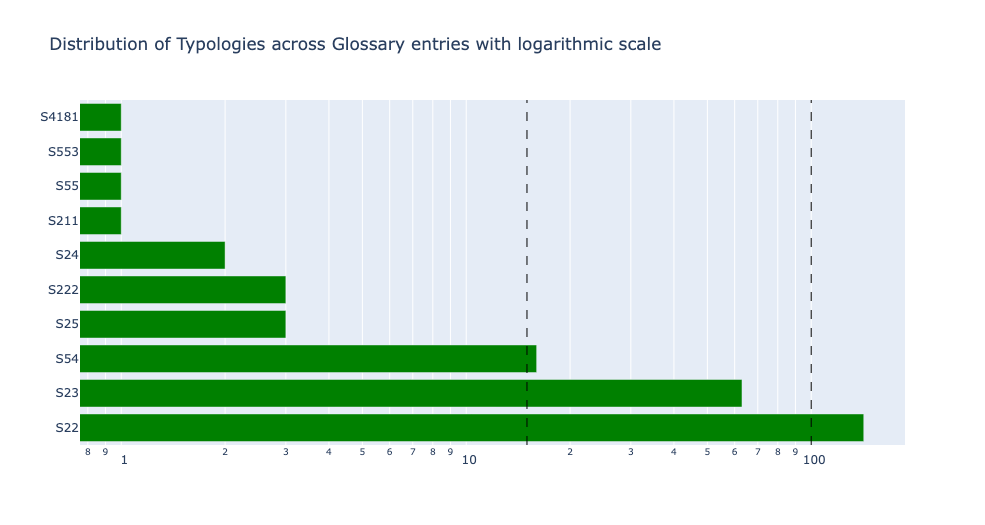
\includegraphics[width=12cm]{Lat14087_graphs/typologies_glosses.png}
  \caption{Répartition des typologies présentes dans le glossaire Lat14087.}
  \label{fig:typologiesLat14087}
\end{figure}

\begin{figure}[H]
  \centering
  \includegraphics[width=12cm]{Lat14087_graphs/proportion_typologies_forms_glosses.png}
  \caption{La taille des entrées est généralement aseez modérée (F3), à l'exception de la typologie S23 (définition) qui, comme on peut s'y attendre, est plus étendue et se compose de propositions complètes.}
  \label{fig:tailletypologiesLat14087}
\end{figure}

Comme prévu, la plupart des entrées sont réparties entre les catégories suivantes : Synonymes(S22), Définitions(S23), Étymologie(S54), Division d'un mot en ses composantes(S24), Hyponyme expliqué par un hypéronyme(S222) et Dérivation lexicale(S24). Nous avons également rencontré des cas moins fréquents, tels qu'une occurrence de la typologie S211 (Traduction du grec au latin (ou vice versa) pour le mot \og{}circumflexus\fg{}), une occurrence de la typologie 553 (Nom propre) et une occurrence particulièrement intéressante, celle de la typologie S4181 : \og{}4181 Corrélation entre explication et citations\fg{}:

Plus précisément, le lemme \textit{fluctuo} se trouve annoté dans un cas d'usage de ce verbe dans les \textit{Carmina Burrana} \\

\begin{figure}[H]
  \centering
  \includegraphics[height=1cm, width=18cm]{Lat14087_graphs/4181_Lat14087.png}
  \caption{L'entrée de la typologie S4181}
  \label{fig:4181Lat14087}
\end{figure}

Carmina burrana 108 (O langueo!), strophe 1, vers 2-3 (pag.: 404) \footnote{référence trouvé dans la LLT : éd. B. K. Vollmann (Bibliothek deutscher Klassiker - Bibliothek des Mittelalters, 13, 1987)} : 

1. VACILLANTIS Trutine libramine \\
mens suspensa \textbf{fluctuat et estuat;} \\
\textbf{in diuersa rapior,} \\
ratione cum Dione \\
dimicante. crucior. \\


et semble être une annotation plus spontanée, avec la suite du \textit{carmen} profane et religieux,  là ou les autres témoins, qui glosent plusieurs fois le même verbe (en raison de la répétition des mêmes exemples dans le livre) présentent une uniformité frappante avec des gloses autour de \og{}titubo\fg{} et \og{}dubito\fg{}. Même la note marginale du Lat7499 choisit d'illustrer l'usage du verbe avec un exemple explicatif et non littéraire :

\begin{table}[htbp]
  \resizebox{\textwidth}{!}{
    \begin{tabular}{|c|c|c|c|c|}
      \hline
      \textbf{Témoin} & \textbf{LemmaID} & \textbf{Lemma} & \textbf{Annotation\_id} & \textbf{Annotation} \\
      \hline
      Lat14087 & p459\_l07\_o10 & fluctuo & N/A & \textit{uacillo, indiuersa rapior} \\
      \hline\hline
      VLO41 & p450\_l09\_o03 & Fluctuo & p450\_l09\_o03\_a & \textit{dubito ł titubo} \\
      VLO41 & p462\_l29\_o11 & Fluctuo & p462\_l29\_o11\_a & \textit{titubo} \\
      VLO41 & p464\_l11\_o03 & fluctuo & p464\_l11\_o03\_a & \textit{titubo dubito} \\
      \hline\hline
      Bamberg & p450\_l09\_o03 & fluctuo & p450\_l09\_o03\_a & \textit{titubo}\\
      Bamberg & p459\_l07\_o11 & fluctuo & p459\_l07\_o11\_a & \textit{titubo} \\
      Bamberg & p462\_l29\_o11 & fluctuo & p462\_l29\_o11\_a & \textit{titubo} \\
      \hline\hline
      Lat7499 & p450\_l09\_o03 & fluctuo & p450\_l09\_o03\_a &  \textit{dubito ł titubo} \\
      Lat7499 & p462\_l29\_o11 & Fluctuo & p462\_l29\_o11\_a & \textit{titubo} \\
      Lat7499 & p462\_l29\_o11 & Fluctuo & p462\_l29\_o11\_b & \parbox{6cm}{\raggedright \textit{Fluctuo ÷ dubito : fluctuat enĩ mare qđo undat ñ est serenũ}} \\
      Lat7499 & p464\_l11\_o03 & fluctuo & p464\_l11\_o03\_a & \textit{titulo dubito} \\
      Lat7499 & p450\_l09\_o03 & Fluctuo & p450\_l09\_o03\_a & \textit{dubito ł titubo} \\
      \hline
    \end{tabular}
  }
\end{table}


Dans ce contexte, retrouver et comparer les lemmes et leurs annotations était une tâche rapide, grâce à l'indexation et à la possibilité de recherche en \og{} plein text \fg{} offertes par les éditions numériques en XML TEI. \\

Pour conclure cette brève analyse statistique individuelle du glossaire et des possibilités qu'il offre pour la lecture proche ou la caractérisation d'un témoin, il est important d'examiner la portée du texte couverte par les entrées. Le glossaire a-t-il conservé du matériel uniquement provenant de la première partie de l'œuvre, où la répartition est équilibrée? Pour répondre à cette question, nous avons utilisé l'alignement des lemmes selon l'édition de Keil afin de diviser la quantité d'annotations \og{}par page de Keil\fg{} en tant que référence stable pour évaluer la répartition du matériel inclus dans le glossaire. 

\begin{figure}[H]
  \centering
  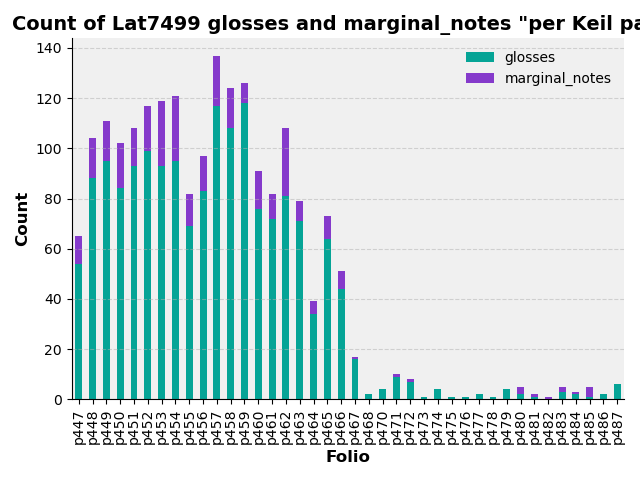
\includegraphics[height=9cm, width=12cm]{Lat14087_graphs/distribution_glosses_marginal_Keil.png}
  \caption{Répartition quantitative des entrées du glossaire Lat14087 selon la pagination de Keil. }
  \label{fig:KeilLat14087}
\end{figure}

De ce qu'il paraît, la répartition des entrées dans le glossaire n'est pas concentrée uniquement au début du livre (qui se termine à la page 467 de l'édition de Keil), mais présente des fluctuations, avec un pic à la page 458. Étant donné que le glossaire en question est relativement petit, ne comportant que trois pages, il est difficile d'évaluer ce graphique de manière isolée. Cependant, grâce à cet alignement, nous sommes en mesure de mettre tous les témoins sur un pied d'égalité en utilisant la même échelle de comparaison, ce qui nous permet de suivre la quantité et la répartition globale des annotations et d'observer les tendances. \\


\subsection{Étude individuelle : le VLO41}

Le témoin Vossianus Latinus 41 constitue un cas d'étude individuel particulier, car il s'agit du premier manuscrit que nous avons étudié dans le cadre du mémoire de M1 et présente un caractère unique grâce aux plusieurs mains qui l'ont copié. Par conséquent, nous avons réalisé des analyses complémentaires par rapport aux autres témoins sur les différentes mains présentes dans ce manuscrit, élucidant le caractère des diverses\og{}collections d'annotations \fg{}.\\ 


\textsc{Répartition des annotations}

L'approche typologique des gloses va au-delà du simple classement et permet de mettre en évidence les préoccupations des glossateurs en arrière-plan, ainsi que la spécificité de leurs enseignements \cite{cinato2011perspectives} démarche particulièrement pertinente dans le cas des sources de type $\Gamma$, telles que le Vossianus Latinus 41. La distinction des couches d'annotations non contemporaines, bien que délicat et chronophage, est inextricablement liée à la transmission des gloses\footnote{cf. aussi la méthodologie du projet \href{https://www.marginalscholarship.nl/what-is-this/about-the-data-recorded-here/}{Marginal Scholarship} = \og{} While it is our intention to distinguish different layers of marginal activity and describe them as separate units, this proved too time consuming for the purpose of the database. When we were able to make out clear units, for example because they were chronologically wide apart, we described them as such, but when the layering was too difficult to analyse, we described them as one layer, with additional remarks in order to point this out.\fg{}}. Ces couches d'annotations peuvent être considérées comme des méta-données relevant notamment de l'étude paléographique (la distinction des écritures joue un rôle essentiel dans cette démarche), et revêtent une importance primordiale dans l'analyse des témoins glosés. En effet, la superposition de différentes couches de gloses dans un même manuscrit témoigne souvent de son étude en différents lieux et à différentes époques. Afin de rendre compte de la perspective diachronique au sein de la collection, il est donc nécessaire d'établir une chronologie relative des mains qui ont contribué à l'annotation du para-texte.\\

Une facette spécifique \og{} Acteur \fg{} est prévue \textit{a priori} par Franck Cinato pour les mains différentes, en fonction du rôle de chaque glosateur, d'une échelle allant du 1 à 3 où:

\begin{itemize}
    \item A1 : Glossateur-copiste
    \item A2 : Glossateur-compilateur
    \item A3 : Glossateur-exégète
\end{itemize}


L'absence d'expérience préalable dans notre démarche et le caractère encore limité de notre échantillon de données nous ont conduits à ne pas effectuer une attribution \textit{a priori} de rôles. Cependant, nous avons utilisé des outils numériques pour mener une analyse exploratoire des statistiques basées sur l'attribution des différentes mains, dans le but de déterminer certaines caractéristiques propres à chaque glosateur. Les outils numériques se révèlent en effet particulièrement adaptés à la manipulation à grande échelle et à la visualisation des données multidimensionnelles, comme les réseaux de gloses présents dans le Vossianus Latinus 41. Ainsi, cette fois nous nous efforçons d'observer de manière spécifique les différents mouvements successifs d'annotations dans le manuscrit, ainsi que les préoccupations propres aux glossateurs-compilateurs.\\

\textsc{Mouvements d'annotation}

Pour notre première visualisation, nous nous sommes intéressés aux variables suivantes : la quantité de gloses écrites par et par folio, ce qui donne deux graphiques complémentaires (Figure 2.5 a et b).

\begin{figure}[H]
    \begin{subfigure}{0.55\textwidth}
    \centering
    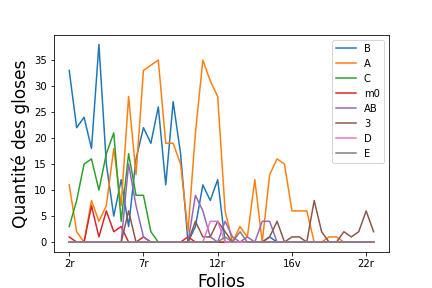
\includegraphics[width=8.5cm]{VLO41_graphs/line_plot_hands_folios.png}
    \caption{line plot}
    \end{subfigure}
    \begin{subfigure}{0,55\linewidth}
    \centering
    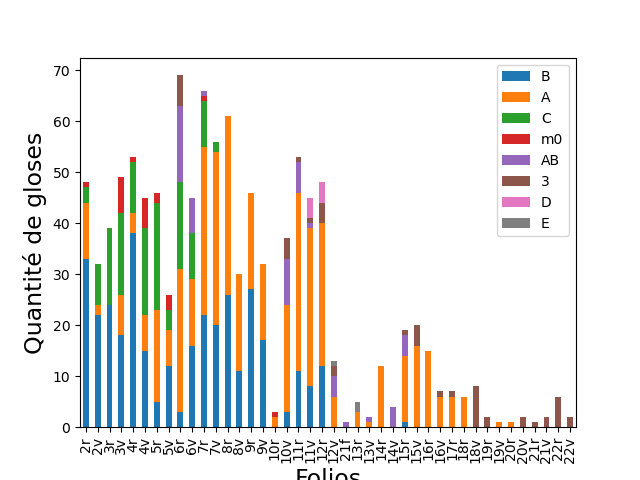
\includegraphics[width=8.5cm]{VLO41_graphs/stacked_barplot_hands_folios.png}
    \caption{Stacked bar}
    \end{subfigure}
    \caption{Dans le premier graphique, une ligne correspond à une main en traçant sa contribution per folio. Le deuxième prend les mêmes variables et en donne la densité de la contribution de chaque main.}
    \label{fig:VLO41distribitionhands}
\end{figure} 

\begin{figure}[H]
    \centering
    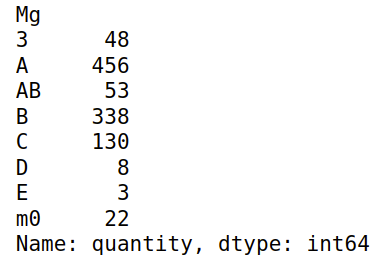
\includegraphics[width=6cm, height=4cm]{VLO41_graphs/quantite_mains.png}
    \caption{Somme des gloses écrites par chaque main. \og{}Mg\fg{}=  Main de glosateur.}
\end{figure}


Le premier graphique permet de suivre l'évolution de l'activité de chaque scribe au fil des folios, en visualisant l'intensité de leur contribution. Il offre une vue d'ensemble du mouvement des mains dans le manuscrit. La seconde visualisation, complémentaire à la première, permet d'analyser plus en détail le pourcentage de contribution de chaque scribe par folio, permettant ainsi de détecter les tendances émergentes. Grâce à ces deux graphiques, des observations générales peuvent être formulées et des conclusions peuvent être tirées sur le comportement des scribes et les schémas d'écriture présents dans le manuscrit : \\

\begin{itemize}
\item La quantité de gloses diminue progressivement au fil des folios, confirmant ainsi la tendance générale qui montre une concentration des gloses au début des manuscrits.
\item La visualisation met en évidence le rôle marginal des quatre dernières mains. La main B est dominante pour les cinq premiers folios\footnote{Il convient de préciser que les mains sont nommées selon leur ordre d'apparition dans le manuscrit et non en fonction de leur importance ou de la quantité de gloses produites.}. Ensuite, elle coexiste avec la main A jusqu'au folio 10v, où la main A devient dominante jusqu'à la fin du manuscrit.
\item Trois mains, A, B et C, se distinguent comme les principaux glossateurs du VLO41. Alors que les deux premières ont une répartition plus équilibrée sur l'ensemble de la surface glosée, avec la main A prenant le relais après la main B, la troisième main, C, se concentre exclusivement sur les 14 premiers folios.
\item On observe une absence générale de gloses sur le folio 10r.
\end{itemize}

Les observations quantitatives sont des outils d'analyse qui, seules, ne peuvent pas être considérées comme une source d'interprétation suffisante. Cependant, lorsqu'elles sont combinées avec des observations qualitatives, elles apportent des nuances et contribuent à des interprétations intéressantes, notamment dans le cas de corpus hétérogènes et multivariables. Il est essentiel de prendre en compte ces deux aspects pour approfondir notre compréhension du sujet étudié. \\

Les deux dernières observations nécessitent une exploration plus approfondie. En ce qui concerne l'activité de la main C, il semble qu'elle ait principalement utilisé le manuscrit à des fins pédagogiques, en se concentrant sur les premières pages du traité comme matériel de cours. Cette interprétation est étayée par les \textit{notae} de construction\footnote{Les informations sur les signes proviennent de : \cite{steinova2016notam}} présentes sous sa plume, qui sont visibles aux folios 2v, 6r et 6v, mais qui cessent complètement après le folio 7r, soit peu de temps avant la fin de l'intervention de la main C.\\

\begin{figure}[H]
    \centering
    \includegraphics[width=15cm, height=5cm]{6v_notae.png}
    \caption{Négatif du folio 6v avec échantillon des \textit{notae} de la main C}
\end{figure}

\begin{itemize}
    \item Ligne 2 à la fin :  \fbox{s} pour \textit{scribe} $\rightarrow$ signe indiquant le début d'un extrait ou d'une leçon, dans ce cas en combinaison avec un autre signe indiquant la fin. Une alternative pourrait être \textit{lege}.
    \item Ligne 4 au milieu : \fbox{d} pour \textit{dimitte} $\rightarrow$ signe indiquant la fin d'un extrait ou d'une leçon ; dans ce cas, en combinaison avec un autre signe indiquant le début.
    \item Ligne 3 au milieu : variation du \textit{trigon} $\rightarrow$ Quant au trigon et à ses variations comme le quadrigon, il s'agit d'un caractère assez divers, qui sert souvent comme signe d'attention lors de la lecture. 
     \item Ligne 4 au début :  \fbox{n} sur \textit{quasi} $\rightarrow$ En l'absence d'une explication concrète de ce que \og{}n\fg{} pourrait signifier, nous ne souhaitons pas forcer une interprétation.
    \item Ligne 1 au début : le chiffre  \fbox{VI} ; En général, les chiffres ou les premières lettres de l'alphabet sont utilisés comme signes de l'ordre syntaxique au sein de la proposition\footnote{\cite{lemoine1989symptomes}, p.152 \og{}[...]il arrive souvent avec les manuels scolaires du haut Moyen Âge de porter des signes (doubles points, triples points, points-virgules, etc.) qui, portés sur certains mots du texte, ont pour but de faciliter la compréhension de la phrase latine : on relie le substantif et l’adjectif, le sujet et le verbe, le verbe et son complément etc. Une autre catégorie de signes de construction, que H. Korhammer appelle système séquentiel, consiste en lettres de l’alphabet qui, disposées sur les différents mots de la phrase, permettent au lecteur de lire celle-ci dans l’ordre de sa langue vernaculaire.\fg{}}.  
\end{itemize}

Pour ce qui est de l'absence générale de gloses dans le folio 10r, cette coupure coïncide avec le changement de cahiers dans la composition du manuscrit. Entre les folios 9v et 10r, une feuille est visiblement déchirée, en réduisant le quinion initial en quaternion. Nous pouvons supposer soit que cette partie du texte n'a pas porté autant de gloses que les passages avoisinants, soit que le déchirement d'un feuillet, une intervention codicologique externe a eu un impact sur les pratiques d'annotation du manuscrit. Une fois que plusieurs témoins auront été transcrits et comparés, une image plus claire pourra se dessiner sur cette particularité.\\

\textsc{Typologies générales vs. typologies particulières}

\begin{figure}[H]
\centering
\begin{subfigure}{0.80\textwidth}
  \centering
  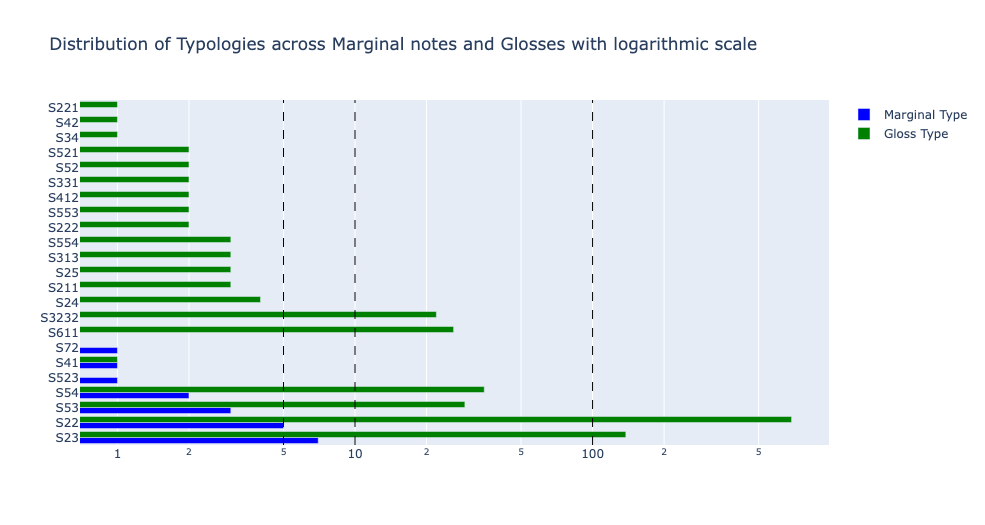
\includegraphics[height=8cm]{VLO41_graphs/general_graphs/comp_typologies_glosses_marginalia.png}
  \caption{Répartition des typologies des gloses dans le VLO41 selon leur taille.}
  \label{fig:general_typologies}
\end{subfigure}
\\
\hfill
\begin{subfigure}{0.45\textwidth}
  \centering
  \includegraphics[height=6cm]{VLO41_graphs/general_graphs/proportion_typologies_forms_glosses.png}
 \caption{Répartition selon la taille des typologies des gloses dans le VLO41.}
  \label{fig:VLO41typologies_glosses}
\end{subfigure}
\begin{subfigure}{0.45\textwidth}
  \centering
  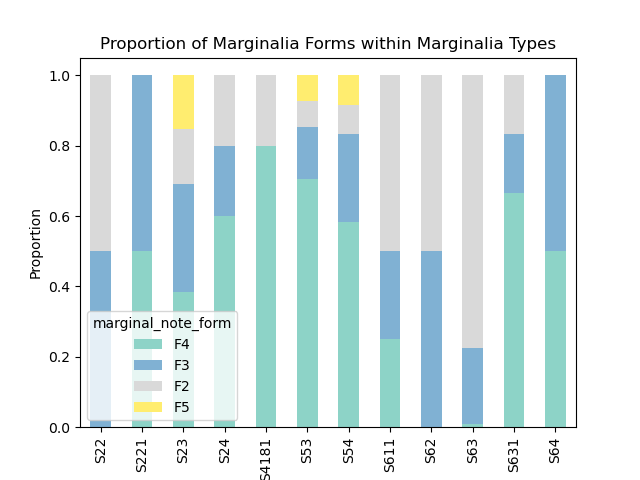
\includegraphics[height=6cm]{VLO41_graphs/general_graphs/proportion_typologies_forms_marginalia.png}
    \caption{Répartition des typologies des \textit{marginalia} dans le VLO41 selon leur taille.}
  \label{fig:VLO41typologies_marginalia}
\end{subfigure}
\caption{Répartition des typologies dans le VLO41.}
\label{fig:VLO41typologies}
\end{figure}


Abordons maintenant à la facette suivante. En ce qui concerne la typologie des gloses, nous avons d'abord cherché à fournir un aperçu de leur répartition indépendamment des couches d'annotations. Ensuite, nous avons dressé un panorama général de leur répartition par main, illustré par le graphique de la Figure \ref{fig:VLO41distribitionhands}. Nous avons choisi un circular barplot, présenté par ordre croissant, afin d'éviter de mettre trop d'accent sur les valeurs élevées, que ce soit pour les mains ou les types de gloses. Cela est dû à l'hétérogénéité des variables, qui rendrait tout autre type de graphique moins approprié.\\


\begin{figure}[H]
    \centering
    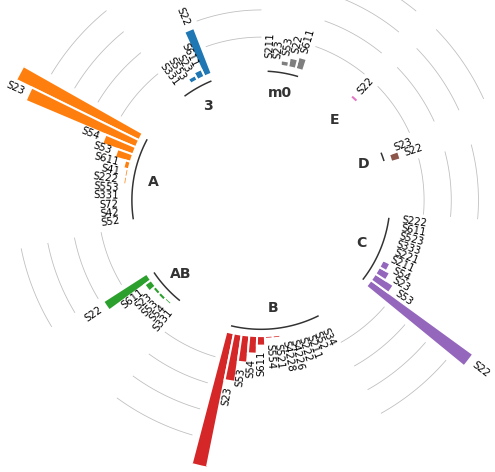
\includegraphics[width=12cm, height=11cm]{VLO41_graphs/circular_barplot.png}
    \caption{Circular barplot pour la distribution hiérarchique du type de gloses utilisé par main.}
\end{figure}

Il devient évident que toutes les mains privilégient une certaine typologie de gloses, contribuant à des taux différents, en tenant compte de la quantité de gloses écrites par chaque main. \\


\begin{itemize}
    \item  \fbox{S22} Synonyme ;
    \item  \fbox{S23} Définition ;
    \item   \fbox{S53} Précisions sur le texte, glose élucidant le sens ;
    \item   \fbox{S54} Étymologie ;
    \item   \fbox{S611} Correction critique du texte (y compris des ajouts postérieurs).
\end{itemize}

Un tableau complet se trouve ci-dessous : 
\begin{figure}[H]
    \begin{subfigure}{0.40\textwidth}
    \centering
    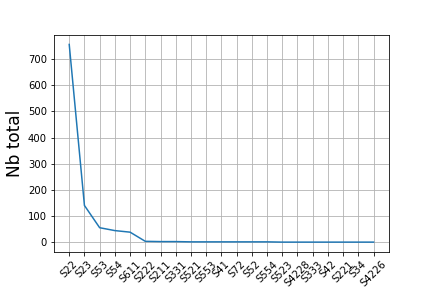
\includegraphics[width=9cm]{VLO41_graphs/typologie_privilegiee.png}
    \caption{Typologies privilégiées}
    \end{subfigure}
    \begin{subfigure}{0,40\linewidth}
    \centering
    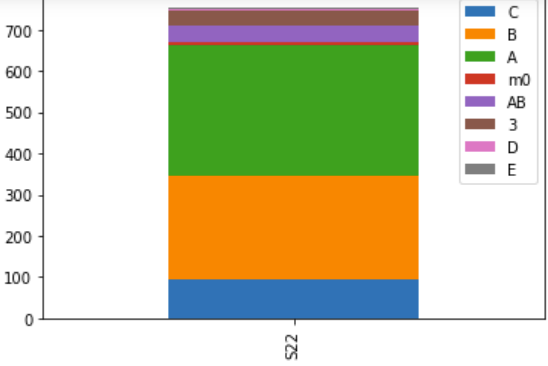
\includegraphics[width=7cm]{VLO41_graphs/typologies/S22.png}
    \caption{Synonyme}
    \end{subfigure}
    \begin{subfigure}{0,40\linewidth}
    \centering
    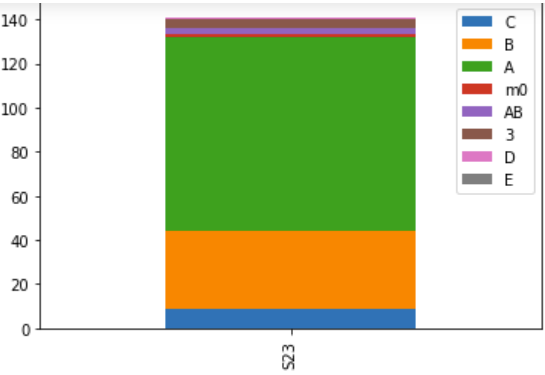
\includegraphics[width=7cm]{VLO41_graphs/typologies/S23.png}
    \caption{Définition}
    \end{subfigure}
     \begin{subfigure}{0,40\linewidth}
    \centering
    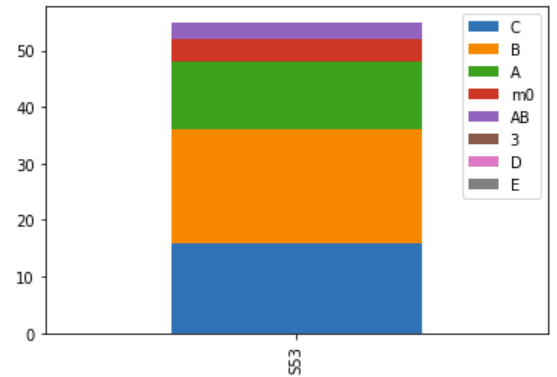
\includegraphics[width=7cm]{VLO41_graphs/typologies/S53.png}
    \caption{Élucide les ambiguïtés du texte}
    \end{subfigure}
    \begin{subfigure}{0,40\linewidth}
    \centering
    \includegraphics[width=7cm]{VLO41_graphs/typologies/S54.png}
    \caption{Étymologie}
    \end{subfigure}
        \begin{subfigure}{0,80\linewidth}
    \centering
    \includegraphics[width=7cm]{VLO41_graphs/typologies/S611.png}
    \caption{Intervention éditoriale: corrections}
    \end{subfigure}
\end{figure} 

\clearpage

En plus des tendances générales, qui sont les cas de base lors d'une annotation, ce sont les typologies moins fréquentes qui donnent le caractère distinctif d'une campagne d'annotation ou le \og{}style\fg{} d'un glosateur. Plus précisément :

Pour A:

\begin{itemize}
    \item \fbox{S41} Signe de construction syntaxique (2 occurences)
    \item \fbox{S42} Mot(s) explicitant la construction (1 occurence)
\end{itemize}

Pour B:

\begin{itemize}
    \item \fbox{S554} Commentaire mythologique (2 occurences)
    \item \fbox{S521} \og{} quia\fg{} gloses (2 occurences)
    \item \fbox{S34} Indication d'adverbe (1 occurence)
    \item \fbox{S4226} supplétive par un adverbe (1 occurence)
    \item \fbox{S4228} supplétive par un verbe (1 occurence)
\end{itemize}

Pour C:

\begin{itemize}
    \item \fbox{S333} morphologie du \textit{modus} (2 occurences)
    \item \fbox{S221} négation d'un antonyme (1 occurence)\\
\end{itemize}

Si peu nombreuses que soient ces occurrences, les groupes concernés, grâce à leur spécificité, permettent de déterminer un certain nombre de caractéristiques relatives soit à la collection, soit aux préoccupations personnelles de chaque glosateur. Entre autres, la main A se soucie assez spécifiquement de la construction syntaxique des lemmes qu'elle glose. Il en va de même pour la main C et ses explications sur le \textit{modus} du verbe, ou pour la main B et son souci des adverbes. Ces typologies appartiennent plutôt à la sphère de l'explication grammaticale et révèlent les objectifs pédagogiques. Ces gloses sont soit le produit original de chaque glosateur, qui a apporté ses propres observations, soit suivent une tradition spécifique présente dans la circulation de ce texte glosé.\\

Il n'en va pas de même pour les typologies S554, S521 et S221. Un commentaire mythologique, comme celui concernant les lemmes \textit{cupido} (quidam deus) et \textit{flamen} (sacerdotum iouis significat), peut être originaire d'une collection ou d'une source spécifique, telle qu'un glossaire. De même, pour les \og{}quia-gloses\fg{}, un commentaire explicatif introduit par \textit{quia} (=parce que), et pour la négation d'un antonyme, qui n'apparaît pas aussi souvent que le synonyme exact d'un lemme. De plus, une comparaison entre les témoins peut permettre de mieux comprendre le taux d'originalité et le \og{}poids\fg{} qu'on peut attribuer à chaque glose\footnote{cf la classification de : \cite{steinova2021glosses}, Introduction}.\\

Une fois que davantage de témoins ont été transcrits et qu'une collection parallèle de gloses a été établie, ces observations initiales se prêteront à une analyse plus fondée. Quoi qu'il en soit, cet exemple est révélateur de la manière auxiliaire dont une analyse exploratoire peut contribuer à une étude proche plus centrée, surtout lorsqu'il s'agit de données hétérogènes et à facettes multiples.\\



\section{Étude comparative}


Nous avons décidé d'étudier les spécificités des manuscrits BambergMsc30 et Lat7499 à travers cette étude comparative et de ne pas y dédier des chapitres entiers. Cependant, des graphiques analytiques concernant leur typologie et leur taille sont présentés dans les \hyperref[annexes]{Annexes} pour consultation.\\ 


Quels sont alors les objectifs de cette analyse comparative ? Que cherchons-nous à accomplir ? Notre étude vise à examiner la typologie, la variété et l'évolution des annotations dans les manuscrits de la période médiévale précoce. Nous souhaitons comprendre les pratiques d'annotation et en tirer des interprétations significatives. Nous visons également à répondre à des questions posées par Mariken Teeuwen sur l'interaction entre l'espace intérlinéaire et marginal \footnote{Lors de sa communication au séminaire HTL-Labex du 03/02/2023 intitulé \og{}Glossing Between the Lines
\fg{}\url{https://htl.cnrs.fr/mc-events/seminaire-htl-labex-marieken-teeuwen-uni-leiden/?mc_id=83}.} à savoir \og{}How does the density of the glossing compare?\fg{}, \og{}How does the consistency of the copying process compare?\fg{}, \og{}How does the profile of the glosses compare?\fg{} et, \og{}How does the material in the margin
compare to that between the lines?\fg{}. Ce sont des questions-pivot qui ont animé notre méthodologie comparative. \\

Examinons tout d'abord nos données et les premiers descripteurs macro-quantitatifs très généraux :\\

\begin{tabular}{|c|c|c|c|c|}
\hline
 Descripteurs & Lat14087 & VLO41 & BambergMsc30 & Lat7499 \\
\hline
folios annotés & 3/3 & \textbf{42/63} & 30/30 & 39/39 \\
lemmas & 233 & 984 & \textbf{2031} & 1903 \\
unique lemmas & 6 & 21 & 33 & \textbf{68} \\
\hline\hline
gloses & 233 & 972 & 1763 & \textbf{1768} \\
gloses en notes tironiennes & N/A & N/A & 272 & N/A \\
typologie plus fréquente & S22 & S22 & S22 & S22 \\
forme plus fréquente & \textbf{F3} & F2 & F2 & F2 \\
marginalia & N/A & 20 & \textbf{570} & 327 \\
typologie plus fréquente & N/A & S23 & \textbf{S63} & S23 \\
forme plus fréquente & N/A & F4 & F2 & \textbf{F5} \\
\hline\hline
typologies uniques & 11 & 23 & 35 & \textbf{44} \\
\hline
\end{tabular} \\

Tout d'abord, en ce qui concerne la quantité de folios annotés, il semble que la totalité des folios soient annotés (à différents degrés de densité), à l'exception du VLO pour lequel les gloses couvrent respectivement 42 sur 63 folios, laissant 21 folios entièrement dépourvus d'annotations. En ce qui concerne le nombre de lemmes, le manuscrit \textit{BambergMsc30} se distingue en enregistrant le plus grand nombre avec 2040 lemmes, tandis que le manuscrit \textit{Lat14087} en compte le moins, avec seulement 233 lemmes. Pour ce qui est des lemmes uniques, c'est-à-dire ceux qui ne figurent pas dans l'édition critique de Keil, c'est le manuscrit \textit{Lat7499} qui se démarque avec 69 lemmes uniques, tandis que les autres manuscrits en possèdent moins de 50.\\

Du côté de la typologie, la plus fréquente pour les gloses dans tous les manuscrits étudiés est \textbf{S22}, qui correspond aux synonymes, ce qui est pleinement attendu compte tenu de la fonction des gloses. Les gloses de cette typologie sont principalement sous forme de morphèmes (F2). En revanche, en ce qui concerne les notes marginales, le manuscrit \textit{BambergMsc30} se distingue par le nombre le plus élevé de \textit{marginalia}, avec 568 occurrences, tandis que les autres manuscrits en comptent moins de 400. Il est important de noter que la plupart des \textit{marginalia} pour \textit{BambergMsc30} appartiennent à la typologie \textbf{S63}, qui correspond aux titres/indexations marginales, qu'elles soient postérieures ou non à la copie du manuscrit, et qui servent à s'y retrouver dans le texte. Les autres manuscrits ont principalement la typologie \textbf{S23}, qui correspond aux définitions. Il est clair que le manuscrit \textit{Lat7499} contient les \textit{marginalia} les plus longues, sous forme de paragraphes (F5), tandis que celles des autres manuscrits ne dépassent pas la proposition (F4) pour cette même typologie. Cette constatation initiale en dit long sur le caractère du \textit{Lat7499}, qui, comme nous le savons, abrite le commentaire de Rémi d'Auxerre, où apparemment un plus grand espace est consacré dans la marge pour éclairer et élaborer sur la définition d'un lemme, ce qui semble raccord avec le rôle des marginalia en générale.\\

Enfin, une constatation intéressante est que le manuscrit \textit{Lat7499} compte le plus grand nombre de typologies uniques dans l'ensemble de ses annotations (gloses et marginalia), avec 43 typologies uniques, tandis que les autres en comptent respectivement 35, 23 et 11. On peut avancer que la taille des lemmes uniques est proportionnelle au nombre total de lemmes, et ainsi cette tendance incrémentale ne présente aucune anomalie. Nous pourrons utiliser cet élément ultérieurement pour calculer la variance des annotations pour chaque manuscrit.



\subsection{Le rôle des gloses et des marginalia}

Une question épineuse qui se pose dans la recherche des manuscrits glosés concerne le rôle des annotations marginales et interlinéaires, ainsi que leur éventuelle différence. Lors d'une présentation récente au séminaire du laboratoire HTL intitulée \og{}Glossing between the Lines\fg{}, Mariken Teeuwen a laissé cette question ouverte, car elle n'a pas pu parvenir à une conclusion définitive avec la lecture proche. Grâce à nos outils numériques, nous sommes désormais en mesure de répondre à cette question en regroupant la fréquence d'occurrence de chaque typologie dans l'ensemble de notre jeu de données.\\

\begin{figure}[H]
    \centering
    \begin{subfigure}[b]{\textwidth}
        \includegraphics[height=10cm]{comparative_graphs/gloss_typologies_all.png}
        \caption{Répartition des typologies pour les gloses interlinéaires.}
    \end{subfigure}
    \vfill
    \begin{subfigure}[b]{\textwidth}
        \includegraphics[height=9cm]{comparative_graphs/marginalia_typologies_all.png}
        \caption{Répartition des typologies pour les annotations marginales.}
    \end{subfigure}
    \caption{Quantité des typologies pour l'ensemble des données ; visualisation en échelle logarithmique.}
    \label{fig:entire-figure}
\end{figure}

Selon les graphiques des typologies des gloses et des \textit{marginalia}, nous pouvons faire les observations suivantes. Les typologies représentées en couleur verte dépassent la médiane et sont considérées comme les plus symptomatiques de l'ensemble du jeu de données, selon notre analyse. \\

Ainsi, nous dressons une liste comparative des typologies qui comptent plus de 10 occurences :



\begin{table}[H]
\centering
\begin{tabular}{|c|c|}
\hline
\rowcolor{gray!20}
\textbf{Marginal Typologies} & \textbf{Gloss Typologies} \\
\hline
{\textbf{63} Titulation, Indexation marginale} & {\textbf{22} Synonyme} \\
\hline
\textbf{23} Définition littérale & \textbf{23} Définition littérale \\
\hline
\textbf{53} Élucide les ambiguïtés du texte & \textbf{53} Élucide les ambiguïtés du texte \\
\hline
\textbf{5} Explicative &{\textbf{3232} Explicite le contexte d'un pronom} \\
\hline
{\textbf{22} Synonyme} &{\textbf{54} Étymologique} \\
\hline
{\textbf{54} Étymologique} & {\textbf{611} Correction critique du texte ou Correction rédactionnelle} \\
\hline
{\textbf{631} Résumé du contenu} & {\textbf{25} Décomposition d'un mot} \\
\hline
{\textbf{62} Collation et variantes} & {\textbf{211} Traduction du grec au latin (ou l'inverse)} \\
\hline
{\textbf{4181} Corrélation entre explication et citations} & {\textbf{415} Corrélation entre un verbe et son sujet} \\
\hline
\end{tabular}
\end{table}

Concernant le rôle des annotations marginales et interlinéaires, le tableau comparatif met en évidence la présence de typologies communes aux deux pratiques. Parmi ces typologies, nous retrouvons S22 (Synonymes), S23 (Définition), S53 (Élucide les ambiguïtés du texte) et S54 (Étymologique). Elles peuvent être considérées comme des fonctions annotatives génériques, indépendantes de l'emplacement spécifique de l'annotation. Par contre, il existe des typologies uniques pour chaque pratique, qui aident à élucider le rôle des pratiques d'annotation. \\

Considérons les différentes catégories :\\

Les annotations interlinéaires se concentrent principalement autour de la catégorie des annotations lexicales (Catégorie 2). Outre les typologies communes mentionnées précédemment, nous observons les typologies suivantes : S25 (décomposition d'un mot en ses composantes) et S211 (traduction du grec au latin). De plus, dans la catégorie des annotations morphologiques (Catégorie 3), nous trouvons spécifiquement la typologie -S3232 (Explicite le contexte d'un pronom)-, qui n'est pas présente dans les typologies les plus caractéristiques des annotations marginales. À partir de ces deux catégories, nous pouvons conclure que les annotations interlinéaires s'intéressent davantage à une échelle micro, en se focalisant sur le lemme en tant qu'unité lexicale en élucidant son con-texte.\\

En ce qui concerne la typologie suivante, à savoir S4 (Syntaxique), nous constatons que les annotations marginales se concentrent principalement sur la typologie S4181 (corrélation entre explication et citations), qui tend à être plus développée, tandis que les annotations interlinéaires privilégient la typologie S415 (corrélation entre un verbe et son sujet). Une fois de plus, nous observons une échelle macro pour les annotations marginales et une échelle micro pour les annotations interlinéaires.\\

Enfin, la catégorie 5, (Explicative), n'apparaît que dans les annotations marginales. Nous remarquons également une accumulation de catégories S6 (Ecdotique-critique) pour les annotations marginales, à savoir : S62 (Collation et variantes), S63 (Titulation et indexation marginale) et S631 (Résumé du contenu), qui se concentrent davantage sur le lemme en tant qu'unité sémantique englobant un rôle moins restreint par sa réalité textuelle. En revanche, la typologie S611 (Correction critique du texte) est présente dans les annotations interlinéaires et se concentre davantage sur l'état du texte lui-même.\\

Étant donné que la plupart du temps (mais pas toujours), les annotations marginales viennent compléter et enrichir les annotations interlinéaires, nous pouvons conclure que leur différence réside dans la manière dont le lemme est perçu dans chaque cas, à savoir en tant qu'unité lexicale dans son contexte, versus en tant qu'unité sémantique, voire méta-textuelle (pour S63) ou inter-textuelle (pour S62). Bien sûr, nous avons pris en compte les typologies les plus fréquentes et il s'agit en général d'une généralisation, mais cela correspond à l'ensemble de données que nous avons examiné.\\

Bien évidemment, regrouper et interpréter le rôle des annotations selon les typologies est très utile pour élucider les pratiques d'annotation, mais nous pouvons aller plus loin. En ce qui concerne les typologies spécifiques rares ou qui présentent un intérêt particulier, nous avons également la capacité de les isoler en fonction de nos objectifs et de nos questions de recherche afin de les examiner de plus près. Par exemple, il est possible d'extraire toutes les annotations liées à la collation (S611) ou à l'intertextualité et à la détection des sources (4181) afin de contribuer à l'établissement d'un \textit{apparatus fontium}. De même, nous pouvons sélectionner les annotations relatives aux traductions en latin, en grec ou dans une langue vernaculaire (S222), ainsi que les gloses portant sur la mythologie ou la littérature latine (S554). Cette approche nous permet de cibler et d'analyser de manière plus précise les types d'annotations qui correspondent à nos besoins et à nos intérêts de recherche.


\subsection{Recoupements entre témoins et le \og{}socle commun\fg{} des annotations.}

Grâce à l'indexation et les outils numériques à notre disposition\footnote{Le notebook avec les manipulations et l'étude croisée se trouve \href{https://github.com/malamatenia/Eutyches/tree/main/comparative_mss_analysis}{ici}.}, nous avons pu comparer les lemmes de chaque manuscrit deux à deux en utilisant la colonne \textit{lemma\_id}, afin d'identifier les lemmes partagés. Ensuite, nous avons appliqué une condition où la typologie et la forme devaient être identiques pour isoler les lemmes dont les gloses présentent à la fois la même typologie et la même taille. Outre l'analyse quantitative et statistique, ces jeux de données sont extrêmement utiles dans le processus de collation et la lecture approfondie du matériel d'annotation. Tous les fichiers CSV contenant les \href{https://github.com/malamatenia/Eutyches/tree/main/comparative_mss_analysis/common_lemmas_csv}{lemmes communs} et \href{https://github.com/malamatenia/Eutyches/tree/main/comparative_mss_analysis/identical_glosses_csv}{lemmes identiques} avec leurs gloses sont disponibles dans notre dépôt Github et peuvent être consultés.\\


\begin{table}[H]
    \centering
    \begin{tabular}{|c|c|c|}
        \hline
        \rowcolor{gray!20}
        \textbf{Manuscript Pair} & \textbf{Lemmas in Common} & \textbf{Identically Glossed Lemmas} \\\hline
        \hline
        Lat14087 - VLO41 & 141 & 30 \\ \hline
         Lat14087 - Lat7499 & 168 & 45 \\
        \hline
        Lat14087- Bamberg & 165 & 48 \\\hline
        VLO41 - Bamberg & 564 & 242 \\\hline
        VLO41 - Lat7499 & 643 & 234 \\\hline
        Bamberg - Lat7499 & 1095 & 521  \\\hline
        all without glossary & 497 & 119
        \\\hline
        all with glossary & 101 & 6   
        \\\hline
    \end{tabular}
    \caption{Récoupement des lemmas en commun et des lemmas dont les gloses partagent la même typologie et taille - entre les témoins.}
    \label{tab:lemma_comparison}
\end{table}

L'une des questions qui nous a préoccupés était l'existence d'un \og{}noyau commun\fg{} de lemmes annotés que nous pourrions identifier comme une \og{} collection \fg{} de la tradition manuscrite stable, transmise dans tous les témoins, et qui confère ainsi un caractère constant au \og{}de uerbo augmenté\fg{} tel que nous l'avons défini dans notre modèle conceptuel.\\

En appliquant la même méthode à l'ensemble des manuscrits, nous avons découvert que, en l'absence du glossaire, les trois manuscrits partagent \textbf{497 lemmes en commun} (\textbf{25\%} du nombre total du témoin le plus densement glosé), parmi lesquels \textbf{119} sont identiques en termes de typologie et de taille. En incluant le glossaire (ce qui réduit encore davantage les possibilités de correspondance), nous avons identifié \textbf{102 lemmes communs} (qui correspond au \textbf{5\%} du nombre total de lemmes dans le témoin le plus densement glosé), dont \textbf{5} sont identiques.\\

Il est intéressant d'explorer comment ces résultats peuvent être utilisés pour effectuer une comparaison qualitative de nos témoins, établir des corrélations et observer les tendances qui en découlent.\\


\begin{figure}[H]
    \includegraphics[height=3cm, width=17cm]{comparative_graphs/5_identical.png}
    \caption{Les six lemmes \og{}identiques\fg{} parmi tous les témoins.}
\end{figure}


Ce petit recoupement entre les témoins offre une excellente opportunité de mettre en évidence les avantages de l'approche graphématique et la non-normalisation/correction dans la transcription des témoins, notamment lorsque les mêmes signes abréviatifs sont utilisés pour le même lemme ou la même glose (ou non, cf. \og{}probus\fg{}). Par exemple, les termes \og{}percucio/percutio\fg{}, \og{}ubero/exubero\fg{} et \og{}paciscor/pasciscor\fg{} sont symptomatiques des divergences entre témoins, précieux pour la collation. De même, le lemme \og{}e(f)futilis\fg{} et ses gloses offrent une excellent occasion pour une lecture approfondie.\\

En effet, dans sa collation et ses commentaires sur les symptômes irlandais du manuscrit Oxford, Bodl., Auct F. 4. 32 par rapport au BnF Lat. 7499 la \og{}tradition française\fg{}, Louis Lémoine soulève une remarque pertinente concernant le lemme\og{}uas\fg{}\footnote{\cite{lemoine1989symptomes}, p. 145}:

\og{}f°5r : nomen \textbf{uasss} apud mrgilium gl. \textbf{effutilis}.\\

\textbf{Il y a confusion entre futilis, «qui laisse échapper ce qu’il contient» (Gaffiot) et effutilis}, «dit au hasard». S. Gall 904, f° 56b (Keil I, 131.25) porte une glose v. irl. traduite «nom donné à un vase de fond pointu qui sert aux offrandes des dieux (païens)», qui éclaire la gl. v. br. de BN lat. 10290, f° 37r : aperth lestr, «vase de sacrifice», glose à futilis. Le manuscrit de Paris porte aussi la gl. inanis et, en marge, Vir gilius non futilis auctor. Toutes ces gloses viennent de Servius, Énéide XI.339 : NON FVTILIS AYCTOR non inanis : nam futtile uas quoddam est lato ore, fundo angusto, quo utebantur in sacris Vestae, etc.12. Faut-il supposer que la glose d’Oxford vient d’une grammaire de Priscien? Cela n’est pas sûr, car uasss pour uasis rappelle les graphies fautives signalées plus haut et qui trahissent la copie hâtive et peu soignée. En 7499, f° 77r, la fin de glose à effutio : inaniter loquor, effutilis loquax, uacuus, inanis, uel genus uasculi ex quo offerebant pagani suis diis (...) correspond assez bien comme à la c’est glose le irl. cas de dans S. Gall, Oxford mais et Virgile dans Paris n’y est BN pas lat. nommément...\fg{}\\

Pierre-Yves Lambert, confirme cette confusion du sens du lemme \og{}effutilis \fg{}: \\

\og{} de l'origine insulaire, cette fois pour le manuscrit BN Lat. 10290 de Priscien :  \footnote{\cite{lambert1982gloses}, p.206-207} :
\og{} [...] 37 b 31, lire \textit{aperlhleslr} et non a \textit{perih lestr} (F.) ; glose « efutilis ». La glose correspondante du manuscrit irlandais nous apprend ce qu’était le \textit{uas futilis} : \textit{nomen do lestur chorthón bis oc-edpartaib do deib}, « nom donné à un vase au fond pointu qui sert aux offrandes aux dieux (païens) » [...]\fg{} \\


ce qui justifie la leçon \og{}efutilis\fg{} avec un \og{}f\fg{} et la glose \og{}uacuus\fg{} au lieu de \og{} uanus \fg{} du VLO41. Effeectivement, notre propre manuscrit \og{}franaçais\fg{} le Lat7499 comporte en marge l'annotation suivante: \\

\og{}  effutilis loquax uacuus \\
 inanis\textbf{ uel genus uasculi} \\
 \textbf{ex quo offerebant pagani} \\
\textbf{suis diis} hoc ẽ exile ex \\
inferiori parte ⁊ latum \\
 in supreriori uelut staubus?\fg{} \\
 
Cet exemple, combiné à d'autres observations plus approfondies sur les différents témoins, peut servir à vérifier l'appartenance à une famille spécifique\footnote{Nous sommes d'accord avec Lémoine (1989), p.145 qui souligne que, malheureusement, en l'absence d'une édition complète des commentaires carolingiens à Eutychès, comparable à celle dont nous disposons pour le \textit{De natura Rerum} de Bède, nous devons souvent nous contenter d'émettre des hypothèses.}.

\subsubsection{Gloses \og{}tironiennes\fg{}: entre Bamberg et Lat7499}

Un de nos témoins, comme il est le cas avec 
Une des observations que nous étions capable de faire grâce au déchiffrement des notes tironiennes de M Cinato, est de confirmer qu'une grande partie des  gloses en latin étaient  en notes tironiennes. 
Les notes tironiennes sont un ensemble de symboles utilisés, par exemple, pour économiser de l'espace ou pour ajouter discrètement des marques destinées aux copistes ou aux étudiants d'un texte (usque hic). Cependant, lorsque des collections entières de gloses sont rédigées en notes tironiennes, cela soulève des questions sur leur veritable fonction. Nous nous interrogeons donc : est-ce que la présence de notes tironiennes indique que le public de l'époque carolingienne était plus familier avec la sténographie et que le milieu de production de ce témoin était plus \og{}académique\fg{}? Étaient-elles utilisées uniquement dans un but d'économie d'espace ? Est-ce que les copistes recopiaient \textit{ad hoc} en notes tironiennes ou bien les exemplaires originaux comportaient-ils déjà des notes tironiennes qui ont été transcrites telles quelles ?\\

Pour le moment, nous sommes en mesure de fournir des analyses statistiques sur ces notes. Parmi les 1095 lemmes partagés entre les manuscrits Lat7499 et BambergMsc30, 152 correspondent à des gloses tironiennes côté BambergMsc30. Si l'on souhaite exprimer ces chiffres en pourcentage, cela représente 13,88\% des gloses partagées entre le Lat7499 et le BambergMsc30. Cependant, sans comparaison avec d'autres paires de manuscrits, nous ne sommes pas en mesure d'évaluer si ce chiffre est élevé ou faible.\\

Il est important de souligner que les notes tironiennes ne se limitent pas aux gloses. Sur un total de 270 notes tironiennes présentes dans le manuscrit BambergMsc30, 13 lignes avec présence des notes tironiennes se trouvent dans les annotations marginales. Une étude plus approfondie, qui dépasse le cadre de ce mémoire de Master 2, pourrait éventuellement permettre de mieux comprendre leur rôle et leur relation avec le Lat7499 et d'autres témoins appartenant à la même \og{} famille \fg{}.

\begin{figure}[H]
    \includegraphics[height=4cm, width=16cm]{comparative_graphs/tironian_examples.png}
    \caption{Les sept premiers exemples des notes tironiennes dans BambergMsc30 avec leur équivalent dans le Lat7499.}
\end{figure}


Notre analyse des notes tironiennes n'est pas exhaustive, ce qui limite nos conclusions pour le moment. Cependant, d'après la partie transcrite par M. Cinato, il est évident que les notes tironiennes du manuscrit BambergMsc30 ne transcrivent pas toujours fidèlement les mêmes gloses que celles du Latin7499 \footnote{cette conclusion a été émis par J. Colette pour l'ensemble des annotations, ce qui est globalement vrai \cite{jeudy1974manuscrits},p. 434}. Cette corrélation pourrait éventuellement faciliter la lecture des notes qui n'ont pas encore été transcrites en fournissant les \og{}gloses équivalentes\fg{} du Latin7499. Un csv avec la liste complète des notes tironiennes est disponibles dans notre \href{https://github.com/malamatenia/Eutyches/tree/main/comparative_mss_analysis}{dépôt Github}. \\


\subsection{Questions de densité(s)}


Une façon de définir la densité est la densité visuelle, qui correspond à la quantité d'espace couvert par des annotations sur la page, et la densité d'annotation, qui correspond à la quantité de matériel glosé. Nous aborderons d'abord la deuxième notion.\\

\subsubsection{Densité d'annotation}

Pour mesurer la densité d'annotation, nous avons compté la quantité et le pourcentage de lemmes par mots (du texte principal) par page. La raison pour laquelle nous utilisons les lemmes plutôt que les annotations est que ces dernières peuvent varier en longueur pour chaque lemme (d'un mot à un paragraphe), et ne constituent donc pas une mesure fiable de la densité de l'activité d'annotation en elles-mêmes. Cela nous a permis d'obtenir les graphiques suivants pour nos trois témoins (les pages dont la quantité de lemmes est inférieure à la médiane sont représentées en bleu). \\


\begin{figure}[H]
  \centering
  \begin{subfigure}[b]{0.3\textwidth}
    \centering
    \includegraphics[width=6cm]{VLO41_graphs/general_graphs/lemma_ratio_per_folio.png}
    \caption{VLO41}
  \end{subfigure}%
  \hfill
  \begin{subfigure}[b]{0.3\textwidth}
    \centering
    \includegraphics[width=6cm]{BambergMsc30_graphs/lemma_ratio_per_folio.png}
    \caption{BambergMsc30}
  \end{subfigure}%
  \hfill
  \begin{subfigure}[b]{0.3\textwidth}
    \centering
    \includegraphics[width=6cm]{Lat7499_graphs/lemma_ratio_per_folio.png}
    \caption{Lat7499}
  \end{subfigure}
  \caption{Ratio de lemmes par page.}
\end{figure}


Relecture : Dans l'ensemble, il semble que, par rapport aux VLO41 et Lat7499, Bamberg effectue des annotations de manière plus systématique tout au long des pages du manuscrit, même si la quantité diminue clairement dans la seconde moitié de l'œuvre. Il est également intéressant de comparer comment, pour VLO et Bamberg, le pourcentage de lemmes ne dépasse pas les 34\%, tandis que pour Lat7499, il atteint près de 45\%, ce qui représente un pourcentage significativement élevé. Comparons les folios avec le pourcentage maximal de lemmes pour se faire une idée visuelle de la manière dont ces pourcentages se traduisent en \og{} pages manuscrites \fg{}.\\


\begin{figure}[H]
  \centering
\begin{subfigure}[b]{4.5cm}
\centering
    \includegraphics[width=\textwidth]{comparative_graphs/VLO41_06r.png}
    \caption{VLO41}
  \end{subfigure}%
  \hspace{0.5cm}
  \begin{subfigure}[b]{4.5cm}
  \centering
    \includegraphics[width=\textwidth]{comparative_graphs/Bamberg_75r.jpg}
    \caption{BambergMsc30}
  \end{subfigure}%
  \hspace{0.5cm}
  \begin{subfigure}[b]{4.5cm}
    \includegraphics[width=\textwidth]{comparative_graphs/Lat7499_80r.png}
    \caption{Lat7499}
  \end{subfigure}
  \caption{Les pages les plus densement annotés de chaque témoin.}
  \label{fig:boxplotslemmas}
\end{figure}

Selon que les lemmes acceptent uniquement des annotations marginales ou/et des annotations interlinéaires, l'aspect visuel de cette densité change complètement et il est important de garder cela à l'esprit lorsque nous essayons de définir des termes tels que la \og{}densité\fg{}.

\subsubsection{Densité visuelle}

Une question d'une grande importance dans la recherche des manuscrits glosés concerne l'espace occupé par les annotations (qu'elles soient interlinéaires, marginales ou les deux), car cela peut fournir des informations précieuses sur les pratiques d'annotation, la mise en page ou encore l'origine du \textit{scriptorium} d'un \textit{codex}. Une approche non numérique pour répondre à cette question a été abordée par le projet \og{}Marginal Scholarship\fg{} que nous avons déjà mentionné. Dans leur base de données, ils incluent une estimation de l'espace marginal, qu'ils définissent de la façon suivante :\\


\og{} The ‘most annotated page percentage’*: this percentage expresses the ratio between blank marginal space and marginal space filled with annotations on the page which has the most annotations in the manuscript. In the layout section, we give the percentage of space which is not covered by the text block of the main text: the ‘marginal space percentage’. In the ‘most annotated space percentage’ we give, by estimate, the percentage of marginal space which is taken up by annotations. Thus, if the margins are completely covered with annotations (as, for example, in Codex Paris, BnF, Latin 7505, fol. 25r), this percentage is very high: up to 80 or 90\%. If there are only a few glosses scattered in the margin of even the page which is most densely glossed, the percentage is very low (3 or 2\%). We manually measured a number of samples, and used these to give estimates for our other cases. \fg{}\\ 


L'approche adoptée par leur étude est d'abord empirique, mais elle soulève des questions pertinentes, jetant ainsi les bases d'une démarche numérique plus rigoureuse et ouvre la voie à une exploration plus approfondie et méthodique de \og{}l'espace marginale\fg{}, en exploitant les potentialités offertes par les méthodes numériques.\\

Une méthodologie similaire, mais cette fois entièrement numérique, a été entreprise par l'équipe DIVA dont le projet nous avons déjà cité dans le cadre de notre modèle de segmentation sémantique \footnote{\cite{simistira2016diva}}. Leur méthode de segmentation repose sur l'annotation sémantique (selon les classes définies) des pixels. Ils ont ainsi profité de cette information pour calculer le pourcentage de pixels appartenant à chaque classe par rapport au nombre total de pixels. Pour leur dataset et leur typologie de mise en page (cf Figure \ref{fig:my_figure}), cela correspondait à 41,37\% des commentaires et 56,4\% de texte (cf . Figure \ref{fig:pixel_diva}). \\

\begin{figure}[H]
    \centering
    \includegraphics[height=5cm]{segmentation_imgs/DivaHisDB/percentage_pixels_classes.png}
    \caption{Résultats de l'équipe DIVA sur le pourcentage de pixels appartenant aux classes \og{}commentaire\fg{} et \og{}texte\fg{}.}
    \label{fig:pixel_diva}
\end{figure}

En effet, les outils numériques que nous avons utilisés nous permettent également de déterminer de manière précise le pourcentage d'espace occupé par les notes par rapport au texte principal (qui malheureusement, faute de temps, n'a pas été intégré dans notre pipeline, mais constitue une perspective intéressante). Pour ce faire, nous pouvons exploiter les informations des polygones des lignes qui sont encodées avec l'attribut @facs à l'intérieur de chaque balise <lb/>. Ces balises se distinguent en \og{}principal\fg{} , \og{}interlinear\fg{}  et pour le manuscrit de Bamberg, \og{}tironian\fg{}. Ces informations sont héritées du fichier d'exportation ALTO, soulignant ainsi l'importance de segmenter et de transcrire le texte sur une plate-forme telle que eScriptorium, qui permet de stocker des informations précises sur la mise en page.

\subsubsection{Quantifier l'accrétion de l'information}

Dans la première section théorique de notre étude, nous avons analysé le phénomène d'accrétion successive entre les gloses éparses et le commentaire marginal (cf. figure \ref{fig:exemplesaccretion} et figure \ref{fig:comptypologies}). Cette densité découle de trois méthodes complémentaires : l'accrétion de l'information, la compilation et la collation des témoins contemporains. Le genre du commentaire en général est caractérisé par la \textit{copia}\footnote{\cite{kraus2002introduction}, p.5}, qui se manifeste par un remplissage délibéré de l'espace interlinéaire et marginal. Cette section se concentre ainsi sur une tentative de quantifier ce phénomène dans nos trois témoins, qui s'apprêtent à une telle approche, grâce à leur typologie.\\ 
 
Nous avons décidé d'étudier deux cas, l'un plus général et l'autre plus spécifique. La première hypothèse que nous souhaitons tester et confirmer concerne les pourcentages d'\og{} extension \fg{} de l'information de l'espace interlinéaire à l'espace marginal. À partir d'une lecture approfondie, nous constatons qu'un certain nombre de lemmes continuent d'être annotés de manière plus intensive et que leurs annotations s'étendent jusqu'à la marge. Ainsi, en tenant compte des lemmes communs \og{}par paires\fg{} de nos trois manuscrits glosés, nous allons essayer de détecter le pourcentage de lemmes qui, d'un manuscrit à l'autre, reçoivent une seconde annotation dans l'espace marginal (là où elle n'existait pas). Cette étude présuppose que l'espace interlinéaire est déjà \og{}occupé\fg{} par les gloses interlinéaires. Les résultats statistiques sont en accord avec nos hypothèses théoriques, mais nous pouvons maintenant traduire ces hypothèses en pourcentages.\\

Ainsi, pour le même \og{}fonds commun de lemmes\fg{}, nous constatons que le pourcentage le plus élevé, soit 23,40\% (à savoir des lemmes qui reçoivent une annotation complémentaire), concerne la paire VLO41-->Bamberg, ce qui est logique étant donné que Bamberg est le manuscrit le plus densement glossé et VLO41 le moins densement glossé. Le pourcentage le plus bas, soit 12,15\%, concerne la paire Bamberg --> Lat7499, qui comptait déjà plusieurs annotations marginales. À 20,84\% \\


\begin{figure}[H]
\centering
\includegraphics[height=8cm]{comparative_graphs/incremental_gloss_to_marge.png}
\caption{Évolution de l'incorporation progressive des gloses dans les marges.}
\label{fig:incrementalgloss}
\end{figure}

La deuxième hypothèse concerne l'ensemble du corpus, sans distinction de témoins, et se concentre sur notre typologie la plus fréquente, à savoir les synonymes (S22). La manière la plus simple d'incorporer de l'information est l'accumulation de synonymes. Cette fois-ci, nous avons pris en compte  les trois manuscrits en ordre chronologique, comme un échantillon de \og{}chaîne de production chronologique\fg{}, et nous nous sommes attelés à quantifier, \og{}du début à la fin\fg{}, quelle était la tendance générale en ce qui concerne les synonymes au fil du temps\footnote{Sur un corpus de 234 lemmes. Les conditions pour décrire les tendances sont les suivantes : Si nous avons les séquences F2/F2/F2, F3/F3/F3 ou bien F2/F3/F2 = tendance stable // si nous avons les séquences F3/F3/F2, F3/F2/F2 = tendance décroissante // si nous avons les séquences F2/F2/F3, F2/F3/F3 = tendance croissante}.\\

\begin{figure}[H]
\centering
\includegraphics[height=8cm]{comparative_graphs/tendencies_S22_form_across_mss.png}
\caption{Tendances de la forme du S22 dans notre jeu de données.}
\label{fig:incrementalS22}
\end{figure}


Et si dans l'ensemble, la tendance est stable (55,22\%) et nettement croissante (34,83\%), ce qui confirme l'augmentation claire du nombre de synonymes au fil du temps telle que nous l'observons visuellement, nous souhaitons attirer l'attention sur le pourcentage de 09,95\% des typologies S22 qui diminuent plutôt qu'augmenter, malgré la densité plus faible de ce manuscrit par rapport aux deux autres. Cela est important car, lors d'une lecture approfondie, nous constatons que, dans ces cas (20 lemmes), les leçons des gloses de VLO41 s'écartent complètement des deux autres manuscrits dont les gloses sont presque identiques (à l'exception d'un cas où Bamberg s'accorde avec VLO41, pour le lemme \og{}sollertia\fg{} ).\\

\begin{figure}[H]
    \centering
    \includegraphics[width=14cm]{comparative_graphs/synonyms_decreasing.png}
    \caption{Les 20 gloses-synonymes qui présentent une tendance décroissante entre nos trois témoins glosés.}
\end{figure}

\subsection{Mouvement des annotations}


C'est maintenant le moment de démontrer l'importance de l'indexation pour l'analyse en grande échelle. En raison des différences de mise en page et d'allocation des segments sur les pages des différents manuscrits, les mêmes segments ne se retrouvent pas à la même position d'une page de manuscrit à l'autre. C'est pourquoi indexer les lemmes tout en notant la page de Keil peut nous aider à aligner les informations en utilisant un point de référence commun à tous les témoins. Ainsi, nous pouvons suivre le mouvement et la quantité d'annotations par manuscrit sur une même \og{}carte géographique\fg{} qui s'étend selon les pages de l'édition de Keil.\\



\begin{figure}[H]
    \centering
        \includegraphics[width=17cm]{comparative_graphs/comparative_diffusion_mss_Keil.png}
    \caption{L'alignement des annotations de chaque témoin selon l'édition de Keil.}
    \label{fig:difusion_annotations}
\end{figure}


Ce regroupement revêt une grande importance, car il nous permet d'observer les différents mouvements des annotations, de les comparer entre eux et de confirmer les tendances générales, tout en identifiant les anomalies. Nous avons été agréablement surpris lorsque nous avons tracé ce graphique, car les tendances se sont révélées avec une clarté frappante. Dans la première partie du graphique, on observe clairement une tendance similaire dans la diffusion des annotations, caractérisée par des variations significatives, comme le démontrent les lignes verticales. Plus précisément, nous remarquons six mouvements distincts : quatre phases marquées par une augmentation conséquente des annotations (approximativement aux pages 453, 458, 462 et 465) et deux phases de diminution abrupte (pages 455, 460 et 467). La deuxième diminution abrupte peut être facilement expliquée, car elle correspond à la fin du premier livre. De plus, nous remarquons que le témoin BambergMsc30 est le seul à poursuivre les annotations de façon stable après le premier livre, ce qui le rend unique parmi les autres témoins. Pour ce qui est des autres phases, il est difficile, faute des données, de déterminer leur cause. \\



\subsection{Distance-Variance}


Enfin, une question importante à laquelle nous souhaitons répondre est l'indice de \og{} uniqueness \fg{} des témoins, et comment, au sein d'une vaste tradition de manuscrits comportant des annotations anonymes, il est possible de distinguer les contributions individuelles et originales qui peuvent nous aider à différencier la tradition des gloses anonymes de celle éponyme de Rémi d'Auxerre. L'idée est qu'un commentaire marginal apporte évidemment plus d'éléments d'explication, de collation, de comparaison, etc., et c'est sur cette hypothèse que nous nous baserons pour interpéter nos résultats (voir notre discussion sur le modèle conceptuel de la Figure \ref{fig:modeleconceptuel}). Pour ce faire, nous envisageons d'utiliser le nombre unique de typologies présentes dans les annotations d'un manuscrit, en considérant que plus les annotations présentent de variété, plus la collection s'éloigne des annotations \og{}ordinaires\fg{} telles que les \og{}simples\fg{} synonymes, les définitions, des remarques sur l'étymologie etc. Pour répondre à cette question, nous utiliserons l'indice de Shannon\footnote{\url{https://fr.wikipedia.org/wiki/Indice_de_Shannon}}, qui a été initialement utilisé pour quantifier la biodiversité, mais également employé dans des contextes littéraires\footnote{\cite{bache2013diversity}. Les métriques de biodiversité sont de plus en plus souvent utilisées par la communauté des chercheurs en sciences humaines et computationnelles. Par exemple, récemment, un article de Mike Kestemont et al. dans \textit{Science} a utilisé ces métriques pour estimer le nombre de livres manuscrits perdus\footnote{Kestemont et al., \textit{Science}, 2022}}.\\

Selon sa définition, cet indice offre une mesure de la diversité spécifique d'un milieu, en prenant en compte à la fois le nombre d'espèces présentes (richesse spécifique) et la répartition des individus au sein de ces espèces (équitabilité spécifique). Il s'agit essentiellement d'une mesure d'entropie, représentée par un nombre réel positif généralement compris entre 0 et 5, bien qu'il n'y ait pas de limite théorique maximale. En utilisant un indice de diversité existant, l'entropie indique la quantité d'information fournie par un échantillon selon de la fonction d'information (eg. typologie). Par exemple, l'observation d'un individu d'une espèce considérée comme rare a une faible probabilité et fournit plus d'information que l'observation d'un individu d'une espèce commune. Sa notation formelle est la suivante: \\

\begin{math}
    {\displaystyle H^{\prime }=-\sum _{i=1}^{S}p_{i}\log _{2}p_{i}}
\end{math}

Pour cette raison, nous considérons que cet indice est adapté à notre étude. \\

Afin de mieux comprendre la variance des témoins indépendamment de leur taille, nous avons décidé d'étudier deux cas : l'un avec tous les témoins glosés et l'autre en incluant le glossaire. Le premier graphique, qui concerne nos trois témoins glosés, démontre que même si le Bamberg possède le plus grand nombre de lemmes/annotations, il n'est cependant pas celui qui présente la plus grande variance. En réalité, c'est le Lat7499 qui affiche l'éventail le plus large de typologies uniques. En revanche, lorsque nous regroupons tous les témoins, la non-linéarité se perd dans l'ensemble en raison de la petite taille du Lat14087, et nous avons l'impression que la variance est presque directement proportionnelle à la taille. \\

Parmi eux, Bamberg et Lat7499 se distinguent en présentant la plus grande variance dans la transmission du commentaire de Rémi, selon J Colette. La question qui se pose alors est de savoir quel niveau d' \og{}originalité\fg{} dans les annotations est suffisant pour différencier la tradition des gloses anciennes du commentaire de Rémi. Pour répondre à cette question, il serait nécessaire d'ajouter davantage de témoins, tels que le manuscrit Milan supb71, afin de pouvoir effectuer une distinction plus précise.Une fois que nous aurons étudié l'ensemble des manuscrits glosés, nous serons en mesure d'établir un seuil de \og{}variété\fg{} au-delà duquel l'originalité est plus grande que celle du manuscrit moyen annoté. 

\begin{figure}[H]
    \centering
    \begin{subfigure}{0.45\textwidth}
        \includegraphics[height=6cm]{comparative_graphs/lemmas_variety_shannons_entropy_onlywitnesses.png}
        \caption{Indice de Shannon pour la \textit{variance} des témoins selon leur taille. Échantillon sans le glossaire Lat14087.}
    \end{subfigure}
    \hfill % Horizontal spacing between subfigures
    \begin{subfigure}{0.45\textwidth}
        \includegraphics[height=6cm]{comparative_graphs/lemmas_variety_shannons_entropy_withglossary.png}
        \caption{Indice de Shannon pour la \textit{variance} des témoins selon leur taille.}
    \end{subfigure}
    \caption{Mésures de \textit{variance}.}
    \label{fig:variance}
\end{figure}
  

Notre objectif final est de comprendre comment nous pouvons appréhender la notion de proximité/similarité lorsqu'il s'agit de manuscrits glosés. Intuitivement, on pourrait penser qu'il s'agit du nombre de lemmes/gloses partagés, mais ce nombre n'est pas suffisant dans le cas des gloses, car il occulte les différentes typologies et tailles qui jouent un rôle déterminant dans la similarité effective des gloses. Inspirés une fois de plus par l'approche de Steinova \footnote{\url{https:\/\/db.innovatingknowledge.nl\/edition\/\#left-msstats}}, qui utilisait le nombre de gloses, le nombre de gloses partagées et leur poids moyen (attribué manuellement), nous avons décidé de quantifier deux éléments dans nos ensembles, ceux offerts par notre annotation, à savoir le nombre de gloses partagées et le nombre de gloses identiques en termes de typologie et de taille, et d'utiliser l'indice de similarité de Jaccard pour ce faire.\\

Le coefficient de similarité de Jaccard (ou indice de Jaccard  appelé « coefficient de communauté » dans la publication d'origine) \footnote{\url{https://fr.wikipedia.org/wiki/Indice\_et\_distance\_de\_Jaccard\#}}est généralement utilisé pour comparer la similarité entre deux ensembles. Pour deux ensembles, A et B, l'indice de Jaccard est défini comme le rapport entre la taille de leur intersection et la taille de leur union. Soit deux ensembles \textit{A} et \textit{B}, l'indice est :\\

\begin{math}
 Jaccard(U,V) = \frac{|U \cap V|}{|U \cup V|}
\end{math}

L'extension à \textit{n} ensembles est triviale :\\

\begin{math}
    J(S_1, S_2, \dotsc, S_n) = \frac{|S_1 \cap S_2 \cap \dotsb \cap S_n |}{|S_1 \cup S_2 \cup \dotsb \cup S_n |}.
\end{math}

Dans notre cas, et faute des métriques établies pour ce champ des recherche, nous définissons nous-mêmes l'union et l'intersection, qui ne sont pas les mêmes pour tous les ensembles. L'union correspond aux lemmes identiques (sc. même typologie et taille) et l'intersection correspond aux lemmes communs totaux par paire. De cette façon, la taille de Lat7499 et de Bamberg influence moins l'indice de similarité.\\

\begin{figure}[H]
    \centering
    \begin{subfigure}{0.40\textwidth}
        \includegraphics[width=9cm]{comparative_graphs/jaccard_similarity.png}
        \caption{La matrice de similarité Jaccard entre nos témoins.}
    \end{subfigure}
    \hfill % Horizontal spacing between subfigures
    \begin{subfigure}{0.40\textwidth}
        \includegraphics[width=9cm]{comparative_graphs/dendrogram_jaccard_similarity.png}
        \caption{Le dendrogramme qui résulte de la matrice de similarité.}
    \end{subfigure}
    \caption{La similarité de Jaccard appliquée sur notre jeu de données, fondée sur l'intersection sur l'union des lemmes communs et des gloses identiques. }
    \label{fig:jaccard}
\end{figure}

L'interprétation des résultats issus de la matrice de similarité et du dendrogramme révèle une concordance avec nos intuitions et avec la littérature sur la proximité entre les témoins. Nous observons une proximité plus élevée entre le BambergMsc et le Lat7499 (0.48), suivie du BambergMsc30 et du VLO41 (0.44), puis du Lat14087 et du VLO41 (0.36), et enfin entre le Lat7499 et le VLO41 (0.27). Le dendrogramme qui résulte de la matrice de similarité présente un groupe distinct, celui formé par le VLO41 et le Lat14087, avec une position adjacente pour le moment non déterminée pour le Bamberg et le Lat7499.Il convient de souligner que cette proximité préliminaire nécessitera un affinement des métriques et des informations prises en compte, ainsi qu'une considération impartiale d'un plus grand nombre de témoins glosés du \textit{de uerbo}. Ces résultats peuvent servir de guide pour la constitution des familles de témoins en vue d'une future édition. Toutefois, il est important de présenter ces résultats de manière prudente, sans tirer de conclusions hâtives.\\


\chapter{Conclusions, Limites et Perspectives}

Certes, prétendre avoir couvert en détail tous les aspects abordés dans cet exposé serait impossible. En effet, l'objectif même de cette recherche était d'initier un dialogue ouvert. Par conséquent, nous avons identifié quelques points spécifiques qui pourraient être approfondis dans le cadre d'une extension ou d'une poursuite de ce projet, tout en soulignant ses limites.\\


\section{Questionnements méthodologiques}

Il est essentiel de remettre en question la méthodologie employée, des choix des données à l'encodage et aux outils numériques, afin de répondre de manière la plus adaptée aux questions philologiques et paléographiques qui se posent.\\

La première question qui se pose naturellement dans le domaine des Humanités Numériques concerne les données et la construction du corpus, avec toutes ses biais inhérentes que nous cherchons à explorer. Avec seulement quatre témoins, au sein d'une tradition manuscrite déjà restreinte, avons-nous suffisamment de données pour identifier des tendances claires et établir définitivement un lien entre les manuscrits glosés et les commentaires ? Idéalement, il conviendrait d'élargir le corpus en y incluant tous les témoins glosés, sans tenir compte des critères chronologiques et de provenance mentionnés précédemment, afin d'obtenir une vue d'ensemble de la tradition manuscrite et de l'explorer dans sa totalité \footnote{
Par exemple comparer la \og{}tradition française\fg{} aux témoins d'autres traditions comme celle \og{}allemande\fg{} ou \og{}brettone\fg{} ou bien les influences irlandaises \footnote{voir l'étude comparative de Lémoine : \cite{lemoine1989symptomes}}pour faire des recoupements et faire sortir des tendances.}. Plus nous intégrons de témoins dans notre étude, plus nous serons en mesure de généraliser les observations et de leur conférer une validité plus solide. \\


En même temps, il convient de se demander si nous avons prévu suffisamment de descripteurs pertinents pour caractériser adéquatement le contenu cible, afin d'explorer de manière plus précise les phenomènes de l'annotation marginale en Haut Moyen-Âge. La pertinence, et l'applicabilité du modèle conceptuel mis en avant et son/ses implémention(s) numérique(s) représentent le défi le plus important pour mener à bien notre recherche et obtenir des résultats probants.\\

Une petite remarque concerne la notion et notre tentative de \og{}mesurer\fg{} les influences entre les témoins. Il est souvent le cas que la taille des corpus et l'utilisation de métriques parfois non adaptées biaisent les résultats et les indices de proximité. En l'absence d'expérimentation approfondie sur cette partie, elle demeure encore une piste à optimiser. L'établissement de \og{}poids\fg{} et de métriques permettant de pondérer l'importance des gloses en fonction de leur quantité, de leur typologie ou de leur fréquence \footnote{Ce que Evina Steinovà a réalisé manuellement pour regrouper les gloses en \og{}clusters\fg{} avec des degrés d'influence différents : \cite{steinova2021glosses}} s'avère décisif.\\

Enfin, il est important de toujours garder à l'esprit et de remettre en question la validité de notre approche intellectuelle. Dans le cadre de notre expérience, qui vise à suivre le passage d'un état d'annotation à un autre, nous maintenons notre démarche sans établir a priori une distinction rigide entre la glose anonyme et le commentaire éponyme, car les frontières entre les deux sont majoritairement poreuses. Cependant, il est nécessaire de réfléchir à cette frontière. À partir de quel seuil d'accrétion ou de variance de gloses franchi pouvons-nous parler de deux \og{}genres\fg{} distincts ? Cette question reste ouverte.\\


Comme mentionné précédemment, un grand nombre d'études ont été réalisées au cours de la dernière décennie sur la nature, les spécificités et l'importance des gloses et des annotations marginales, ainsi que sur l'utilisation du format électronique pour leur étude. Cependant, peu d'attention a été accordée à l'élaboration et à l'implémentation numérique de modèles conceptuels visant à converger vers une approche unifiée. À l'exception de l'édition pionnière des gloses du premier livre des \textit{Etymologiae} d'Isidore de Séville réalisée par Evina Steinovà, qui a été entièrement modélisée et encodée à la main, ainsi que du projet \og{}Marginal Scholarship\fg{}, nous n'avons pas trouvé d'autres paradigmes inspirants permettant de mettre nos résultats à l'épreuve et d'évaluer notre approche. Il est essentiel de soumettre nos travaux à l'examen de la communauté scientifique afin de favoriser le progrès de ce domaine de recherche stimulant, ce qui représente à la fois un défi et une opportunité.\\

\section{Nouvelles perspectives comparatives - Portée du projet}


\begin{flushright}\textit{ «Ces exemples  trop  brefs ne  donnent  qu'une  idée  très  approximative  de la richesse de ce commentaire, dont on peut espérer maintenant une bonne édition critique.»}\end{flushright}

\begin{flushright}Jeudy Colette, 1974 \og{} Les manuscrits de l’Ars de uerbo d’Eutychès et le commentaire de Rémi d’Auxerre \fg{}, p.436 \end{flushright}

Enfin, il est essentiel de discuter de l'impact visé par un tel projet sur la tradition manuscrite d'Eutychès, à savoir la création d'une édition propre des gloses. Comme cela a été mentionné à plusieurs reprises, la nature fluide, non linéaire et polyvalent des gloses, ainsi que la complexité de leur transmission , rendent difficile la réalisation d'une édition critique selon les méthodes traditionnelles. Une approche critique alternative consiste plutôt à présenter le matériel sous forme de réseau, qui représente les relations et les similitudes entre les différents témoins. Evina Steinovà décrit le processus de cette approche alternative dans l'introduction de son édition, \footnote{\cite{steinova2021glosses}, Introduction, Network as a model for a Digital Scholarly Edition.}.:

\blockquote{In this framework, several entities (manuscript witnesses, clusters of glosses transmitted together, and chapters of the first book of the Etymologiae) appear as nodes. Glosses that are common to multiple of these entities appear as edges that connect them. In this manner, the users of the edition can access the corpus from several different angles and simultaneously view it in its entirety and dissected into its many constituent entities (clusters, layers of glosses in particular witnesses, and individual glosses).}


\section{Conclusions générales}

Schématiquement, la contribution de ce mémoire de Master se présente comme suit :

\begin{enumerate}
\item La création d'un jeu de données original en libre accès sur HTR-United pour entraîner à la fois des modèles de segmentation de mise en page complexe et des modèles de reconnaissance de caractères;
\item Un modèle de segmentation sémantique YALTAi pour la détection des zones dans des manuscrits glosés, ainsi que deux modèles kraken pour la détection et la classification des baselines des interlignes et des lignes principales (tous prêts à l'émploi;
\item La proposition d'un pipeline numérique semi-automatique avec des compartiments individuels, offrant ainsi plus de flexibilité dans la chaîne de traitement;
\item L'encodage de 3 manuscrits largement glosés avec indexation des lemmes et des descripteurs pour la typologie et la taille des annotations;
\item La proposition d'un modèle conceptuel rudimentaire de notre tradition glosée;
\item Une lecture distante des témoins avec des observations quantitatives préliminaires sur notre jeu des données.
\end{enumerate}

L'objectif de cette étude était de démontrer, tout d'abord sur le plan théorique, l'intérêt de la tradition des manuscrits glosés du \textit{De uerbo} d'Eutychès, en mettant en évidence sa mise en page particulière et ses différents niveaux d'annotation. Ensuite, nous avons exploré les diverses occasions où les outils numériques s'avèrent essentiels pour une description et une manipulation adéquates de documents de cette nature. Notre étude a impliqué l'application de plusieurs technologies à notre cas d'étude, allant de la reconnaissance automatique du texte à l'encodage et à la lecture distante du corpus à travers la visualisation de ses composants. Nous avons également discuté des limites rencontrées et des moyens d'optimiser notre approche.Cette étude préliminaire nous a offert l'opportunité de mener des réflexions approfondies sur la nature intrinsèque de notre corpus des manuscrits glosés. Néanmoins, il convient de souligner que celle-ci soulève plus d'interrogations et de limites qu'elle n'apporte de réponses définitives. En effet, la recherche de solutions numériques met souvent en évidence la complexité inhérente à la nature des données manipulées, ce qui nous pousse à remettre en question nos préjugés initiaux.\\



%Afficher bibliographie
\newpage
\nocite{*}
\printbibliography

% table des figures
\listoffigures

% Appendix
\appendix
\label{annexes}
\section{Graphiques complémentaires pour les manuscrits BambergMsc30 et BnF Lat7499.}

Graphiques pour l'étude individuelle de la typologie et la taille des annotations marginales et interlinéaires des mss. BambergMsc30 et Lat7499.\\

\subsection{BambergMsc30}

\begin{figure}[H]
\centering
\begin{subfigure}{0.80\textwidth}
  \centering
  \includegraphics[height=9cm]{BambergMsc30_graphs/comp_typologies_glosses_marginalia.png}
  \caption{Répartition des typologies des gloses dans le BambergMsc30.}
\end{subfigure}
\\
\hfill
\begin{subfigure}{0.45\textwidth}
  \centering
  \includegraphics[height=6cm]{BambergMsc30_graphs/proportion_typologies_forms_glosses.png}
 \caption{Répartition selon la taille des typologies des gloses dans le BambergMsc30.}
\end{subfigure}
\begin{subfigure}{0.45\textwidth}
  \centering
  \includegraphics[height=6cm]{BambergMsc30_graphs/proportion_typologies_forms_glosses.png}
    \caption{Répartition des typologies des \textit{marginalia} dans le BambergMsc30 selon leur taille.}
  \label{fig:Bambergtypologies_marginalia}
\end{subfigure}
\caption{Répartition des typologies dans le BambergMsc30.}
\label{fig:Bambergtypologies}
\end{figure}

\begin{figure}
  \centering
  
  \begin{subfigure}{\textwidth}
    \centering
    \includegraphics[width=9cm]{BambergMsc30_graphs/distribution_glosses_marginal_folio.png}
  \end{subfigure}
  
  \vspace{0.5cm} % Adjust the vertical spacing if needed
  
  \begin{subfigure}{\textwidth}
    \centering
    \includegraphics[height=7cm]{BambergMsc30_graphs/proportion_typologies_forms_glosses_heatmap.png}
  \end{subfigure}

\end{figure}


\subsection{BnF Lat7499}

\begin{figure}[H]
\centering
\begin{subfigure}{0.80\textwidth}
  \centering
  \includegraphics[height=8cm]{Lat7499_graphs/comp_popular_typologies_glosses_marginalia.png}
  \caption{Répartition des typologies privilegiées des gloses dans le Lat7499 selon leur taille.}
\end{subfigure}
\begin{subfigure}{0.80\textwidth}
  \centering
  \includegraphics[height=8cm]{Lat7499_graphs/comp_rare_typologies_glosses_marginalia.png}
  \caption{Répartition des typologies rares des gloses dans le Lat7499 selon leur taille.}
\end{subfigure}
\\
\hfill
\begin{subfigure}{0.45\textwidth}
  \centering
  \includegraphics[height=6cm]{Lat7499_graphs/proportion_typologies_forms_glosses.png}
 \caption{Répartition selon la taille des typologies des gloses dans le Lat7499.}
\end{subfigure}
\begin{subfigure}{0.45\textwidth}
  \centering
  \includegraphics[height=6cm]{Lat7499_graphs/proportion_typologies_forms_marginalia.png}
  \label{fig:Lat7499typologies_marginalia}
\end{subfigure}
\caption{Répartition des typologies dans le Lat7499.}
\label{fig:Lat7499typologies}
\end{figure}


\begin{figure}
  \centering
  
  \begin{subfigure}{\textwidth}
    \centering
    \includegraphics[width=9cm]{Lat7499_graphs/distribution_glosses_marginal_folio.png}
  \end{subfigure}
  
  \vspace{0.5cm} % Adjust the vertical spacing if needed
  
  \begin{subfigure}{\textwidth}
    \centering
    \includegraphics[height=7cm]{Lat7499_graphs/proportion_typologies_forms_glosses_heatmap.png}
  \end{subfigure}

\end{figure}



\section{Typologie augmentée analytique}

Les notes (ou astérisques) signalent les modifications apportées à la formulation de R. Hofman (1996). Dans cette typologie, les types 1 à 7 désignent les familles, tandis que les sous-groupes (11, 12, etc.) décrivent plus précisément la nature des explications. Seuls les types 1-5 sont considérés comme relevant d'une pratique glossographique ; les types 6 et 7 qui se mêlent aux gloses appartiennent à la classe des annotations critiques (6) ou personnelles (7).

\begin{enumerate}
  \item\textbf{[1.] Prosodique}
  \begin{enumerate}
    \item[11.] Macron ( ̄) ou caron (ˇ) indiquant la quantité d'une syllabe longue ou brève2.
    \item[12.] Commentaire sur la quantité des syllabes.
    \item[13.] Commentaire prosodique élaboré.
  \end{enumerate}
  \item\textbf{[2.] Lexicale}
  \begin{enumerate}
    \item[21.] Traduction (vernaculaire)*
    \item[211.] Traduction du grec au latin (ou l'inverse)*
    \item[22.] Synonyme
    \item[221.] Négation d'un antonyme
    \item[222.] Hyponyme expliqué par un hypéronyme
    \item[23.] Définition littérale3
    \item[231.] Changement de préfixe
    \item[232.] Adjectif glosé par un nom décliné*
    \item[23.] Différences (differentiae)
    \item[24.] Dérivation lexicale*
    \item[25.] Décomposition d'un mot*
  \end{enumerate}
  \item\textbf{[3.] Morphologique}
  \begin{enumerate}
    \item[31.] Grammaire du nomen
    \begin{enumerate}
      \item[311.] Morphologie (déclinaison)
      \begin{enumerate}
        \item[3111.] Nominatif
        \item[3112.] Vocatif
        \item[3113.] Génitif
        \item[3114.] Datif
        \item[3115.] Accusatif
        \item[3116.] Ablatif
      \end{enumerate}
      \item[312.] Nombre
      \item[313.] Genre et autres points morphologiques
    \end{enumerate}
    \item[32.] Grammaire du pronomen
    \begin{enumerate}
      \item[321.] Spécifie le pronom (en général)
      \item[322.] Pronom relatif
      \begin{enumerate}
        \item[3221.] Antécédent d'un pronom relatif (spécifique)
        \item[3222.] Antécédent d'un pronom relatif repris d'une glose précédente.
        \item[3223.] Interprétation ou équivalent lexicale de l'antécédent d'un pronom relatif
        \item[3224.] Pronom relatif sans antécédent identifiable
      \end{enumerate}
      \item[323.] Autres pronoms
      \begin{enumerate}
        \item[3231.] Pronom démonstratif pour un autre
        \item[3232.] Explicite le contexte d'un pronom
        \item[3233.] Substitution du pronom avec changement de cas
      \end{enumerate}
    \end{enumerate}
    \item[33.] Grammaire du verbe et participe
    \begin{enumerate}
      \item[331.] Morphologie verbale (générale)
      \item[332.] Morphologie du tempus
      \item[333.] Morphologie du modus
      \item[334.] Morphologie du participe et du gérondif
    \end{enumerate}
    \item[34.] Indication d'adverbe
    \item[35.] Explicite une conjonction
    \item[36.] Explicite une préposition
    \item[37.] Explicite une interjection
  \end{enumerate}
  \item\textbf{[4.] Syntaxique}
  \begin{enumerate}
    \item[41.] Signe de construction syntaxique
    \begin{enumerate}
      \item[411.] Corrélation entre adjectif/préposition et substantif
      \item[412.] Corrélation du complément du nom (?)
      \item[413.] Corrélation entre un pronom relatif et son antécédent
      \item[414.] Corrélation entre un autre pronom et un nom
      \item[415.] Corrélation entre un verbe et son sujet
      \item[416.] Rétablissement d'un ordre de lecture
      \item[417.] Corrélation des éléments de structure d'une proposition
      \item[418.] Corrélation entre deux propositions
      \begin{enumerate}
        \item[4181.] Corrélation entre explication et citations
        \item[4182.] Autres mises en corrélation
      \end{enumerate}
      \item[419.] Mot supplétif à un oubli de l'auteur
    \end{enumerate}
    \item[42.] Mot(s) explicitant la construction
    \begin{enumerate}
      \item[421.] Identifie le locuteur ou une citation
      \item[422.] Supplétives
      \begin{enumerate}
        \item[4221.] Par un nom ou pronom au nominatif
        \item[4222.] Par un nom ou pronom au génitif
        \item[4223.] Par un nom ou pronom au datif
        \item[4224.] Par un nom ou pronom à l'accusatif
        \item[4225.] Par un nom ou pronom au vocatif (?)
        \item[4226.] Par un adverbe
        \item[4227.] Par un adjectif
        \item[4228.] Par un verbe ou une courte proposition
        \item[4229.] Par une conjonction ou une préposition
      \end{enumerate}
      \item[423.] Modifie un adjectif (?)
      \item[424.] Structure (gloses 'adit')
    \end{enumerate}
  \end{enumerate}
  \item\textbf{[5.] Explicative}
  \begin{enumerate}
    \item[51.] Figures de styles
    \item[52.] Commentaire exégétique (= 541 Hofman)
    \begin{enumerate}
      \item[521.] \og{}Quia-glosses\fg{}, commentaire explicatif introduit par quia (= 542 Hofman)
    \end{enumerate}
    \item[522.] Paraphrase ou glose tirée de Priscien
    \item[523.] Indication (spécification) portée sur le titre d'une œuvre
    \item[53.] Élucide les ambiguïtés du texte (= 543 Hofman)
    \item[54.] Étymologique (= 55 Hofman)
    \item[55.] Encyclopédique (= 56 Hofman)
    \begin{enumerate}
      \item[551.] Géographique (= 561 Hofman)
      \item[552.] Objet inaccoutumé (= 562 Hofman)
      \item[553.] Nom propre (= 563 Hofman)
      \item[554.] Mythologique ou littérature latine (= 572 Hofman)
    \end{enumerate}
    \item[56.] Confrontation entre diverses sources (= 571 Hofman)
  \end{enumerate}
  \item\textbf{[6.] Ecdotique (critique)}
  \begin{enumerate}
    \item[61.] Atéthèse médiévale4
    \begin{enumerate}
      \item[611.] Correction critique du texte ou Correction rédactionnelle
    \end{enumerate}
    \item[62.] Collation et variantes (= 58 Hofman)
    \item[63.] Titulation / indexation marginale (postérieure ou non à la copie); Mise en exergue intertitre, sous-titre, mot (notabilia), etc.
    \begin{enumerate}
      \item[631.] Résumé du contenu (= 52 Hofman)
    \end{enumerate}
    \item[64.] Références croisées (ou interne)5 (= 53 Hofman)
    \begin{enumerate}
      \item[641.] Mot ou signe de renvoi (à une explication)
      \begin{enumerate}
        \item[6411.] Glose 'similiter'
      \end{enumerate}
      \item[6421.] Signe graphique (de renvoi)
      \item[6422.] Renvoi verbal (explicité en toute lettre)
    \end{enumerate}
    \item[65.] Source (= 57 Hofman)
  \end{enumerate}
  \item\textbf{[7.] Informations diverses sur le contexte socio-historiques}
  \begin{enumerate}
    \item[71.] Colophons
    \item[72.] Suscriptions et souscriptions
    \item[73.] Doxologique (formule de prière)
    \begin{enumerate}
      \item[731.] Invocations
      \item[732.] Imprécation (parfois se confond avec l'ex-libris)
    \end{enumerate}
    \item[74.] Pétitions de suffrages
    \item[75.] Autres mentions (jussion, oblation collation, authentification, commémorative, etc.)
    \item[76.] Autres observations (quotidienne, etc.)
  \end{enumerate}
\end{enumerate}



\end{document}
